% ============================================================
% CLASSE DO DOCUMENTO
% ============================================================
\documentclass[a4paper,12pt,twoside]{book}

% ============================================================
% PACOTES DE IDIOMA E CODIFICAÇÃO
% ============================================================
\usepackage[T1]{fontenc}
\usepackage[brazilian]{babel}
\usepackage{indentfirst}

% ============================================================
% LAYOUT, MARGENS E TIPOGRAFIA
% ============================================================
\usepackage[top = 20mm, bottom = 20mm, left = 15mm, right = 10mm]{geometry}
\usepackage{microtype} % tipografia refinada
\usepackage{setspace}  % permite onehalfspacing
\usepackage{fancyhdr}  % cabeçalhos
\usepackage{enumitem}  % controle de listas
\usepackage{titlesec}  % personalização de títulos
\usepackage{makeidx}
\makeindex

% Fonte elegante mas leve (troque se quiser outra família)
% \usepackage{tgpagella}

% ============================================================
% MATEMÁTICA
% (minimalista + robusta = AMS + utilidades)
% ============================================================
\usepackage{amsmath, amssymb, amsfonts, amsthm, mathrsfs}
\usepackage{mathtools} % complementa amsmath
\usepackage{cancel}
\allowdisplaybreaks    % permite quebrar alinhamentos longos

% ============================================================
% FIGURAS, GRÁFICOS E TABELAS
% ============================================================
\usepackage{graphicx}
\graphicspath{{img/}}
\usepackage{booktabs}
\usepackage{multirow}
\usepackage{multicol}
\usepackage{float}
\usepackage{tikz}
\usepackage{pgfplots}
\pgfplotsset{compat=1.18}

% ============================================================
% CORES E LINKS
% ============================================================
\usepackage{xcolor}
\usepackage{hyperref}
\hypersetup{
    hidelinks,
    colorlinks=true,
    linkcolor=black,
    urlcolor=blue,
    breaklinks=true,
    pdftitle={Notas de aula - Cálculo 2},
    pdfauthor={Lucas Leão}
}

% ============================================================
% COMANDOS PERSONALIZADOS — NUMÉRICOS E CONJUNTOS
% ============================================================
\newcommand{\R}{\mathbb{R}}
\newcommand{\Q}{\mathbb{Q}}
\newcommand{\C}{\mathbb{C}}
\newcommand{\K}{\mathbb{K}}
\newcommand{\Z}{\mathbb{Z}}
\newcommand{\N}{\mathbb{N}}

% ============================================================
% COMANDOS PERSONALIZADOS — OPERADORES
% ============================================================
\DeclareMathOperator{\Rea}{Re}
\DeclareMathOperator{\Ima}{Im}
\DeclareMathOperator{\supp}{supp}
\DeclareMathOperator{\sgn}{sgn}
\DeclareMathOperator{\dist}{dist}
\DeclareMathOperator{\Vol}{Vol}
\DeclareMathOperator{\esssup}{ess\,sup}
\DeclareMathOperator{\qtp}{q.t.p.}

% ============================================================
% CORES PARA RASCUNHO (OPCIONAL)
% ============================================================
\newcommand{\cv}{\color{red}}
\newcommand{\co}{\color{orange!90!black}}
\newcommand{\cb}{\color{blue}}
\newcommand{\cg}{\color{green!25!gray}}
\newcommand{\cz}{\color{black}}

% ============================================================
% ESTILOS DE TEOREMA (Robusto + Profissional)
% ============================================================
\definecolor{theoremcolor}{RGB}{0, 80, 80}
\definecolor{definitioncolor}{RGB}{0, 60, 130}
\definecolor{examplecolor}{RGB}{150, 90, 20}
\definecolor{remarkcolor}{RGB}{130, 30, 0}
\definecolor{proofcolor}{RGB}{40, 80, 0}

% Teorema
\newtheoremstyle{color-theorem}
  {10pt}{10pt}{\itshape}{0pt}
  {\color{theoremcolor}\bfseries}{}
  {\newline}{}
\theoremstyle{color-theorem}
\newtheorem{theorem}{Teorema}[chapter]
\newtheorem{lemma}{Lema}[chapter]
\newtheorem{proposition}{Proposição}[chapter]
\newtheorem{corollary}{Corolário}[chapter]

% Definição
\newtheoremstyle{color-definition}
  {10pt}{10pt}{\normalfont}{0pt}
  {\color{definitioncolor}\bfseries}{}
  {\newline}{}
\theoremstyle{color-definition}
\newtheorem{definition}{Definição}[chapter]

% Exemplos
\newtheoremstyle{color-example}
  {10pt}{10pt}{\normalfont}{0pt}
  {\color{examplecolor}\bfseries}{}
  {\newline}{}
\theoremstyle{color-example}
\newtheorem{example}{Exemplo}[chapter]
\newtheorem{exercise}{Exercício}[chapter]
\newtheorem{claim}{Afirmação}[chapter]
\newtheorem{notation}{Notação}[chapter]

% Observações
\newtheoremstyle{color-remark}
  {10pt}{10pt}{\normalfont}{0pt}
  {\color{remarkcolor}\bfseries}{}
  {\newline}{}
\theoremstyle{color-remark}
\newtheorem{remark}{Observação}[chapter]

% ============================================================
% AMBIENTE DE DEMONSTRAÇÃO PERSONALIZADO
% ============================================================
\renewcommand{\qedsymbol}{$\blacksquare$}
\makeatletter
\renewenvironment{proof}[1][\proofname]{%
  \par\pushQED{\qed}%
  \normalfont\topsep6pt\trivlist
  \item[\hskip\labelsep\color{proofcolor}\bfseries #1.]%
}{%
  \popQED\endtrivlist\@endpefalse
}
\makeatother

% ============================================================
% INÍCIO DO DOCUMENTO
% ============================================================
\begin{document}

\frontmatter

\onehalfspacing

% ============================================================
% CAPA — Modelo UNESP / IBILCE / PPG-Matemática
% ============================================================

\begin{titlepage}
\thispagestyle{empty}

\begin{center}
    {\large\bfseries Universidade de São Paulo}\\[2mm]
    {\normalsize Faculdade de Filosofia, Ciências de Letras de Ribeirão Preto \\ Departamento de Computação e Matemática}\\[1mm]
    {\normalsize Matemática Aplicada a Negócios}
\end{center}

\vfill

\begin{center}
    {\Large\bfseries Cálculo Diferencial e Integral II}\\[6mm]
    {\large Notas de Aula}
\end{center}

\vfill

\begin{center}
    {\large Profª. Dra. Michelle Fernanda Pierri Hernandez \\ Lucas Leão}
\end{center}

\vfill

\begin{center}
    {\normalsize Ribeirão Preto}\\
    {\normalsize 2º semestre de 2026}
\end{center}

\end{titlepage}


\tableofcontents


\mainmatter

\chapter{Funções de várias variáveis reais}

Até agora consideramos funcões de uma variável real a valores reais do tipo \[f:I\subset \R \to \R.\] Vamos considerar agora funções que podem depender de mais de uma variável real, ou seja, funções da forma \[F: D\subset \R^n \to \R.\]

A maioria das relações que ocorrem na física, economia e, de modo geral, na natureza é traduzida por funções de duas, três e mais variáveis.

\begin{example}
    \begin{enumerate}
        \item A área de um retângulo depende do seu comprimento e largura, ou seja \[A = A(c,l) = c\cdot l.\]
        \item O volume do cilindro depende de seu raio e altura, \[V = V(r,h) = \pi\cdot r\cdot h.\]
        \item Se o custo de produção \(C\) de um produto depende
            \begin{enumerate}
                \item da qualidade do materia usado \((x)\);
                \item do salário dos funcionários \((y)\);
                \item do tipo de máquina \((z)\);
                \item das despesas de manutenção \((w)\);
                \item da supervisão \((h)\).
            \end{enumerate}
        Então \(C\) é uma função de \(5\) variáveis \(C = C(x,y,z,w,h)\).
    \end{enumerate}
\end{example}

A seguir estudamos funções reais de duas variáveis reais. A generalização para mais variáveis é simples.

\begin{definition}\index{Funções de duas variáveis a valores reais}
    Uma função de duas variáveis reais a valores reais é uma função \(F: D_F \subset \R^2 \to \R\). Ou seja, a cada \((x,y)\in D_F\), a regra \(F\) associa um único valor real \(z = f(x,y)\in\R\).
\end{definition}

A seguir para uma função \(F: D_F\subset\R^2 \to \R\), \(D_F\) é chamado \textbf{domínio}\index{Funções de duas variáveis a valores reais! Domínio} de \(F\) e \[\operatorname{Im}_F = \{z = f(x,y) \in \R : (x,y)\in D_F\}\] é a \textbf{imagem}\index{Funções de duas variáveis a valores reais! Imagem} de \(F\). Além disso, \(x\) e \(y\) são chamadas de \textbf{variáveis independentes} e \(z\) a \textbf{variável dependente}.

\begin{figure}[htbp]
    \centering 
        \begin{tikzpicture}[x=0.75pt,y=0.75pt,yscale=-1,xscale=1]
        %uncomment if require: \path (0,300); %set diagram left start at 0, and has height of 300
        %Straight Lines [id:da2454744672554513] 
        \draw    (30.4,163.6) -- (228.4,163.6) ;
        \draw [shift={(230.4,163.6)}, rotate = 180] [color={rgb, 255:red, 0; green, 0; blue, 0 }  ][line width=0.75]    (10.93,-3.29) .. controls (6.95,-1.4) and (3.31,-0.3) .. (0,0) .. controls (3.31,0.3) and (6.95,1.4) .. (10.93,3.29)   ;
        %Straight Lines [id:da9462448097326388] 
        \draw    (130.4,253.6) -- (130.4,55.6) ;
        \draw [shift={(130.4,53.6)}, rotate = 90] [color={rgb, 255:red, 0; green, 0; blue, 0 }  ][line width=0.75]    (10.93,-3.29) .. controls (6.95,-1.4) and (3.31,-0.3) .. (0,0) .. controls (3.31,0.3) and (6.95,1.4) .. (10.93,3.29)   ;
        %Shape: Polygon Curved [id:ds3375181141487479] 
        \draw  [draw opacity=0][fill={rgb, 255:red, 221; green, 107; blue, 107 }  ,fill opacity=0.44 ] (64.2,118.5) .. controls (84.2,108.5) and (227.2,87.5) .. (207.2,107.5) .. controls (187.2,127.5) and (179.2,182.5) .. (199.2,212.5) .. controls (219.2,242.5) and (94.2,231.5) .. (74.2,201.5) .. controls (54.2,171.5) and (44.2,128.5) .. (64.2,118.5) -- cycle ;
        %Shape: Free Drawing [id:dp9204827379504648] 
        \draw  [color={rgb, 255:red, 255; green, 0; blue, 0 }  ,draw opacity=1 ][line width=3] [line join = round][line cap = round] (78.5,135.95) .. controls (78.5,136.28) and (78.83,136.95) .. (78.5,136.95) ;
        %Shape: Free Drawing [id:dp7849387766178008] 
        \draw  [color={rgb, 255:red, 255; green, 0; blue, 0 }  ,draw opacity=1 ][line width=3] [line join = round][line cap = round] (85,179.45) .. controls (85,179.69) and (85.26,179.95) .. (85.5,179.95) ;
        %Shape: Free Drawing [id:dp46987595803015936] 
        \draw  [color={rgb, 255:red, 255; green, 0; blue, 0 }  ,draw opacity=1 ][line width=3] [line join = round][line cap = round] (103.5,133.45) .. controls (103.74,133.45) and (104,133.71) .. (104,133.95) ;
        %Shape: Free Drawing [id:dp7703404610517858] 
        \draw  [color={rgb, 255:red, 255; green, 0; blue, 0 }  ,draw opacity=1 ][line width=3] [line join = round][line cap = round] (148.5,179.45) .. controls (148.67,179.78) and (148.83,180.12) .. (149,180.45) ;
        %Shape: Free Drawing [id:dp19881301407247098] 
        \draw  [color={rgb, 255:red, 255; green, 0; blue, 0 }  ,draw opacity=1 ][line width=3] [line join = round][line cap = round] (148.5,119.45) .. controls (148.5,119.45) and (148.5,119.45) .. (148.5,119.45) ;
        %Shape: Free Drawing [id:dp5710424755546443] 
        \draw  [color={rgb, 255:red, 255; green, 0; blue, 0 }  ,draw opacity=1 ][line width=3] [line join = round][line cap = round] (168.5,115.45) .. controls (168.5,115.62) and (168.5,115.78) .. (168.5,115.95) ;
        %Shape: Free Drawing [id:dp5794203159577371] 
        \draw  [color={rgb, 255:red, 255; green, 0; blue, 0 }  ,draw opacity=1 ][line width=3] [line join = round][line cap = round] (156,152.45) .. controls (156,152.45) and (156,152.45) .. (156,152.45) ;
        %Shape: Free Drawing [id:dp48323620450280513] 
        \draw  [color={rgb, 255:red, 255; green, 0; blue, 0 }  ,draw opacity=1 ][line width=3] [line join = round][line cap = round] (114,194.45) .. controls (114,194.45) and (114,194.45) .. (114,194.45) ;
        %Shape: Free Drawing [id:dp5146781872742409] 
        \draw  [color={rgb, 255:red, 255; green, 0; blue, 0 }  ,draw opacity=1 ][line width=3] [line join = round][line cap = round] (163.5,208.95) .. controls (163.5,208.95) and (163.5,208.95) .. (163.5,208.95) ;
        %Shape: Free Drawing [id:dp5139020858297133] 
        \draw  [color={rgb, 255:red, 255; green, 0; blue, 0 }  ,draw opacity=1 ][line width=3] [line join = round][line cap = round] (169,133.45) .. controls (169,133.62) and (169,133.78) .. (169,133.95) ;
        %Shape: Free Drawing [id:dp19700765387729546] 
        \draw  [color={rgb, 255:red, 255; green, 0; blue, 0 }  ,draw opacity=1 ][line width=3] [line join = round][line cap = round] (113,146.45) .. controls (113.24,146.45) and (113.5,146.71) .. (113.5,146.95) ;
        %Shape: Free Drawing [id:dp834751610315057] 
        \draw  [color={rgb, 255:red, 255; green, 0; blue, 0 }  ,draw opacity=1 ][line width=3] [line join = round][line cap = round] (118.5,173.45) .. controls (118.5,173.62) and (118.5,173.78) .. (118.5,173.95) ;
        %Shape: Free Drawing [id:dp726934650472843] 
        \draw  [color={rgb, 255:red, 255; green, 0; blue, 0 }  ,draw opacity=1 ][line width=3] [line join = round][line cap = round] (143,136.95) .. controls (143,136.95) and (143,136.95) .. (143,136.95) ;
        %Shape: Free Drawing [id:dp8110315242879534] 
        \draw  [color={rgb, 255:red, 255; green, 0; blue, 0 }  ,draw opacity=1 ][line width=3] [line join = round][line cap = round] (172,186.45) .. controls (172,186.45) and (172,186.45) .. (172,186.45) ;
        %Shape: Free Drawing [id:dp9233705674999151] 
        \draw  [color={rgb, 255:red, 255; green, 0; blue, 0 }  ,draw opacity=1 ][line width=3] [line join = round][line cap = round] (179.5,215.45) .. controls (179.5,215.45) and (179.5,215.45) .. (179.5,215.45) ;
        %Shape: Free Drawing [id:dp5938234305401566] 
        \draw  [color={rgb, 255:red, 255; green, 0; blue, 0 }  ,draw opacity=1 ][line width=3] [line join = round][line cap = round] (141,211.95) .. controls (141,212.12) and (141,212.28) .. (141,212.45) ;
        %Straight Lines [id:da8978492632675772] 
        \draw    (429.9,254.7) -- (429.9,56.7) ;
        \draw [shift={(429.9,54.7)}, rotate = 90] [color={rgb, 255:red, 0; green, 0; blue, 0 }  ][line width=0.75]    (10.93,-3.29) .. controls (6.95,-1.4) and (3.31,-0.3) .. (0,0) .. controls (3.31,0.3) and (6.95,1.4) .. (10.93,3.29)   ;
        %Shape: Free Drawing [id:dp07629673461708475] 
        \draw  [color={rgb, 255:red, 255; green, 0; blue, 0 }  ,draw opacity=1 ][line width=3] [line join = round][line cap = round] (429.3,109.45) .. controls (429.3,109.62) and (429.3,109.78) .. (429.3,109.95) ;
        %Curve Lines [id:da02270658119899094] 
        \draw    (147.3,132.95) .. controls (187.1,103.1) and (310.06,50.48) .. (424.08,107.09) ;
        \draw [shift={(425.8,107.95)}, rotate = 206.86] [fill={rgb, 255:red, 0; green, 0; blue, 0 }  ][line width=0.08]  [draw opacity=0] (8.93,-4.29) -- (0,0) -- (8.93,4.29) -- cycle;

        % Text Node
        \draw (240.24,155.88) node [anchor=north west][inner sep=0.75pt]    {$x$};
        % Text Node
        \draw (126.24,29.88) node [anchor=north west][inner sep=0.75pt]    {$y$};
        % Text Node
        \draw (206,226.4) node [anchor=north west][inner sep=0.75pt]    {$\textcolor[rgb]{0.82,0.01,0.11}{D_{F}}$};
        % Text Node
        \draw (129.96,139.49) node [anchor=north west][inner sep=0.75pt]  [font=\scriptsize,rotate=-359.72]  {$( x,y)$};
        % Text Node
        \draw (425.74,34.88) node [anchor=north west][inner sep=0.75pt]    {$\mathbb{R}$};
        % Text Node
        \draw (439.3,99.4) node [anchor=north west][inner sep=0.75pt]    {$z\ =\ F( x,y)$};
        \end{tikzpicture}
    \caption{Funçaõ de duas variáveis reais}
    \label{fig:variasvariaveis}
\end{figure}

\begin{remark}
    Quando não especificamos o domínio da função, fica subentendido que se trata do ``maior'' subconjunto de \(\R^2\) para o qual a função faz sentido.
\end{remark}

\begin{example}
    Seja \(f(x,y) = \frac{x+y}{x-y}\). Vamos determinar o domínio e a imagem de \(f\).

    Note que devemos ter \[x-y \neq 0 \Rightarrow x\neq y.\] Logo \(D_f = \{(x,y)\in\R^2 : x\neq y\}\).
    \begin{figure}[htbp]
        \centering 
            \begin{tikzpicture}[x=0.5pt,y=0.5pt,yscale=-1,xscale=1]
                %Shape: Rectangle [id:dp9118034779997847] 
                \draw  [draw opacity=0][fill={rgb, 255:red, 74; green, 144; blue, 226 }  ,fill opacity=0.1 ] (51.35,80.33) -- (250.15,80.33) -- (250.15,272.09) -- (51.35,272.09) -- cycle ;
                %Straight Lines [id:da2642326786185505] 
                \draw    (50.4,180.6) -- (248.4,180.6) ;
                \draw [shift={(250.4,180.6)}, rotate = 180] [color={rgb, 255:red, 0; green, 0; blue, 0 }  ][line width=0.75]    (10.93,-3.29) .. controls (6.95,-1.4) and (3.31,-0.3) .. (0,0) .. controls (3.31,0.3) and (6.95,1.4) .. (10.93,3.29)   ;
                %Straight Lines [id:da8917343736599169] 
                \draw    (150.4,273.6) -- (150.4,75.6) ;
                \draw [shift={(150.4,73.6)}, rotate = 90] [color={rgb, 255:red, 0; green, 0; blue, 0 }  ][line width=0.75]    (10.93,-3.29) .. controls (6.95,-1.4) and (3.31,-0.3) .. (0,0) .. controls (3.31,0.3) and (6.95,1.4) .. (10.93,3.29)   ;
                %Straight Lines [id:da21790853074689742] 
                \draw [color={rgb, 255:red, 0; green, 105; blue, 228 }  ,draw opacity=1 ] [dash pattern={on 0.84pt off 2.51pt}]  (61.9,268.83) -- (250.15,80.33) ;

                % Text Node
                \draw (260.24,175.88) node [anchor=north west][inner sep=0.75pt]    {$x$};
                % Text Node
                \draw (146.24,49.88) node [anchor=north west][inner sep=0.75pt]    {$y$};
                % Text Node
                \draw (256,70.32) node [anchor=north west][inner sep=0.75pt]  [color={rgb, 255:red, 74; green, 144; blue, 226 }  ,opacity=1 ]  {$\textcolor[rgb]{0,0.41,0.89}{x\ =\ y}$};
                % Text Node
                \draw (218.8,249.52) node [anchor=north west][inner sep=0.75pt]  [color={rgb, 255:red, 74; green, 144; blue, 226 }  ,opacity=1 ]  {$D_{F}$};
                \end{tikzpicture}
        \caption{Domínio de \(f(x,y) = \frac{x+y}{x-y}\)}
        \label{fig:pol1}
    \end{figure}

    Além disso, \[\operatorname{Im}_f = \left\{z = \frac{x+y}{x-y} : x\neq y\right\} \overbrace{=}^{\text{ (parece) }} \R.\]
\end{example}

\begin{example}
    Seja \(f(x,y) = \sqrt{y-x} + \sqrt{1-y}\). Para determinar o domínio de \(f\) devemos ter
        \begin{enumerate}
            \item[i)] \(y-x \geq 0\), portanto \(y\geq x\);
            \item[ii)] \(1-y \geq 0\), daí \(y\leq 1\).
        \end{enumerate}
    Logo \[D_f = \left\{(x,y)\in\R^2 : y\leq 1 \text{ e } y\geq x\right\}.\]
        \begin{figure}[htbp]
            \centering
                \begin{tikzpicture}[x=0.75pt,y=0.75pt,yscale=-1,xscale=1]
                    %uncomment if require: \path (0,300); %set diagram left start at 0, and has height of 300
                    %Straight Lines [id:da2642326786185505] 
                    \draw    (50.4,180.6) -- (248.4,180.6) ;
                    \draw [shift={(250.4,180.6)}, rotate = 180] [color={rgb, 255:red, 0; green, 0; blue, 0 }  ][line width=0.75]    (10.93,-3.29) .. controls (6.95,-1.4) and (3.31,-0.3) .. (0,0) .. controls (3.31,0.3) and (6.95,1.4) .. (10.93,3.29)   ;
                    %Straight Lines [id:da8917343736599169] 
                    \draw    (150.4,273.6) -- (150.4,75.6) ;
                    \draw [shift={(150.4,73.6)}, rotate = 90] [color={rgb, 255:red, 0; green, 0; blue, 0 }  ][line width=0.75]    (10.93,-3.29) .. controls (6.95,-1.4) and (3.31,-0.3) .. (0,0) .. controls (3.31,0.3) and (6.95,1.4) .. (10.93,3.29)   ;
                    %Straight Lines [id:da21790853074689742] 
                    \draw [color={rgb, 255:red, 0; green, 105; blue, 228 }  ,draw opacity=1 ] [dash pattern={on 0.84pt off 2.51pt}]  (50.56,280.4) -- (250.15,80.33) ;
                    %Straight Lines [id:da7680119420914071] 
                    \draw [color={rgb, 255:red, 0; green, 105; blue, 228 }  ,draw opacity=1 ] [dash pattern={on 0.84pt off 2.51pt}]  (48.37,160.51) -- (248.77,160.91) ;
                    %Shape: Polygon [id:ds21875134066080693] 
                    \draw  [color={rgb, 255:red, 74; green, 144; blue, 226 }  ,draw opacity=1 ][fill={rgb, 255:red, 74; green, 144; blue, 226 }  ,fill opacity=0.14 ] (48.37,160.51) -- (170.16,161.2) -- (50.56,280.4) -- (51.36,160) -- (56.56,160.4) -- cycle ;

                    % Text Node
                    \draw (260.24,175.88) node [anchor=north west][inner sep=0.75pt]    {$x$};
                    % Text Node
                    \draw (146.24,49.88) node [anchor=north west][inner sep=0.75pt]    {$y$};
                    % Text Node
                    \draw (256,70.32) node [anchor=north west][inner sep=0.75pt]  [color={rgb, 255:red, 74; green, 144; blue, 226 }  ,opacity=1 ]  {$\textcolor[rgb]{0,0.41,0.89}{x\ =\ y}$};
                    % Text Node
                    \draw (78.8,253.92) node [anchor=north west][inner sep=0.75pt]  [color={rgb, 255:red, 74; green, 144; blue, 226 }  ,opacity=1 ]  {$D_{F}$};
                    % Text Node
                    \draw (250.8,150.72) node [anchor=north west][inner sep=0.75pt]  [color={rgb, 255:red, 74; green, 144; blue, 226 }  ,opacity=1 ]  {$y\ =\ 1$};
                \end{tikzpicture}                    
            \caption{Domínio de \(f(x,y) = \sqrt{y-x} + \sqrt{1-y}\)}
            \label{fig:raiz1}
        \end{figure}

        Além disso, \[\operatorname{Im}_f = \left\{ z = \sqrt{y-x} + \sqrt{1-y} : y\leq 1 \text{ e } y\geq x \right\} = \{z \geq 0\} = [0\infty).\]
\end{example}

\begin{example}
    Seja \(f(x,y) = x^2 - y^2\). Aqui não temos nenhuma restrição ao domínio, portanto \(D_f = \R^2\). Além disso, \[\operatorname{Im}_f = \left\{ z = x^2 - y^2 : (x,y)\in\R^2 \right\} = \R.\]
\end{example}

\begin{example}
    Consideramos \(f(x,y) = \sqrt{9 - x^2 - y^2}\). Então devemos ter \[9 - x^2 - y^2 \geq 0 \Rightarrow x^2 + y^2 \leq 9.\] Logo \[D_f = \left\{ (x,y)\in\R^2 : x^2 + y^2 \leq 9 \right\}\]
    \begin{figure}[htbp]
        \centering
            \begin{tikzpicture}[x=0.75pt,y=0.75pt,yscale=-1,xscale=1]
                %Straight Lines [id:da2642326786185505] 
                \draw    (50.4,180.6) -- (248.4,180.6) ;
                \draw [shift={(250.4,180.6)}, rotate = 180] [color={rgb, 255:red, 0; green, 0; blue, 0 }  ][line width=0.75]    (10.93,-3.29) .. controls (6.95,-1.4) and (3.31,-0.3) .. (0,0) .. controls (3.31,0.3) and (6.95,1.4) .. (10.93,3.29)   ;
                %Straight Lines [id:da8917343736599169] 
                \draw    (150.4,273.6) -- (150.4,75.6) ;
                \draw [shift={(150.4,73.6)}, rotate = 90] [color={rgb, 255:red, 0; green, 0; blue, 0 }  ][line width=0.75]    (10.93,-3.29) .. controls (6.95,-1.4) and (3.31,-0.3) .. (0,0) .. controls (3.31,0.3) and (6.95,1.4) .. (10.93,3.29)   ;
                %Shape: Circle [id:dp15347112833091703] 
                \draw  [color={rgb, 255:red, 74; green, 144; blue, 226 }  ,draw opacity=1 ][fill={rgb, 255:red, 74; green, 144; blue, 226 }  ,fill opacity=0.19 ] (76.03,180.6) .. controls (76.03,139.53) and (109.33,106.23) .. (150.4,106.23) .. controls (191.47,106.23) and (224.77,139.53) .. (224.77,180.6) .. controls (224.77,221.67) and (191.47,254.97) .. (150.4,254.97) .. controls (109.33,254.97) and (76.03,221.67) .. (76.03,180.6) -- cycle ;

                % Text Node
                \draw (260.24,175.88) node [anchor=north west][inner sep=0.75pt]    {$x$};
                % Text Node
                \draw (146.24,49.88) node [anchor=north west][inner sep=0.75pt]    {$y$};
                % Text Node
                \draw (180.8,91.64) node [anchor=north west][inner sep=0.75pt]    {$\textcolor[rgb]{0.29,0.56,0.89}{x^{2} \ +\ y^{2} \leq 9}$};
            \end{tikzpicture}                    
        \caption{Domínio de \(f(x,y) = \sqrt{9 - x^2 - y^2}\)}
        \label{fig:raiz2}
    \end{figure}
    Além disso \[\operatorname{Im}_f = \left\{ z = \sqrt{9 - x^2 - y^2} : x^2 + y^2 \leq 9 \right\},\] agora, notando que
        \begin{align*}
            0 \leq x^2 + y^2 \leq 9
                & \Leftrightarrow -9 \leq -x^2 - y^2 \leq 0 \\
                & \Leftrightarrow 0 \leq 9 - x^2 - y^2 \leq 9 \\
                & \Leftrightarrow 0 \leq \sqrt{9 - x^2 - y^2} \leq 3,
        \end{align*}
    temos que \(\operatorname{Im}_f = [0,3]\).
\end{example}

\begin{example}
    Seja \(f(x,y) = \frac{1}{\sqrt{4 - x^2 - y^2}}\).

    Devemos ter \[4 - x^2 - y^2 > 0 \Rightarrow x^2 + y^2 \leq 4.\] Logo \[D_f = \left\{(x,y)\in\R^2 : x^2 + y^2 < 4 \right\}.\]
        \begin{figure}[htbp]
            \centering
                \begin{tikzpicture}[x=0.75pt,y=0.75pt,yscale=-1,xscale=1]
                    %Straight Lines [id:da2642326786185505] 
                    \draw    (50.4,180.6) -- (248.4,180.6) ;
                    \draw [shift={(250.4,180.6)}, rotate = 180] [color={rgb, 255:red, 0; green, 0; blue, 0 }  ][line width=0.75]    (10.93,-3.29) .. controls (6.95,-1.4) and (3.31,-0.3) .. (0,0) .. controls (3.31,0.3) and (6.95,1.4) .. (10.93,3.29)   ;
                    %Straight Lines [id:da8917343736599169] 
                    \draw    (150.4,273.6) -- (150.4,75.6) ;
                    \draw [shift={(150.4,73.6)}, rotate = 90] [color={rgb, 255:red, 0; green, 0; blue, 0 }  ][line width=0.75]    (10.93,-3.29) .. controls (6.95,-1.4) and (3.31,-0.3) .. (0,0) .. controls (3.31,0.3) and (6.95,1.4) .. (10.93,3.29)   ;
                    %Shape: Circle [id:dp15347112833091703] 
                    \draw  [color={rgb, 255:red, 74; green, 144; blue, 226 }  ,draw opacity=1 ][fill={rgb, 255:red, 74; green, 144; blue, 226 }  ,fill opacity=0.19 ][dash pattern={on 0.84pt off 2.51pt}] (76.03,180.6) .. controls (76.03,139.53) and (109.33,106.23) .. (150.4,106.23) .. controls (191.47,106.23) and (224.77,139.53) .. (224.77,180.6) .. controls (224.77,221.67) and (191.47,254.97) .. (150.4,254.97) .. controls (109.33,254.97) and (76.03,221.67) .. (76.03,180.6) -- cycle ;

                    % Text Node
                    \draw (260.24,175.88) node [anchor=north west][inner sep=0.75pt]    {$x$};
                    % Text Node
                    \draw (146.24,49.88) node [anchor=north west][inner sep=0.75pt]    {$y$};
                    % Text Node
                    \draw (180.8,91.64) node [anchor=north west][inner sep=0.75pt]    {$\textcolor[rgb]{0.29,0.56,0.89}{x^{2} \ +\ y^{2} < 4}$};
                \end{tikzpicture}                    
            \caption{Domínio de \(f(x,y) = \frac{1}{\sqrt{4 - x^2 - y^2}}\)}
            \label{fig:raiz3}
        \end{figure}

    Além disso, \[\operatorname{Im}_f = \left\{ z = \frac{1}{\sqrt{4 - x^2 - y^2}} : x^2 + y^2 < 4 \right\},\] mas notando que
        \begin{align*}
            0 \leq x^2 + y^2 < 4
                & \Leftrightarrow  - 4 \leq -x^2 - y^2 \leq 0 \\
                & \Leftrightarrow 0 < 4 - x^2 - y^2 \leq 4 \\
                & \Leftrightarrow 0 < \sqrt{4 - x^2 - y^2} \leq 2 \\
                & \Leftrightarrow \frac{1}{\sqrt{4 - x^2 - y^2}} \geq \frac{1}{2},
        \end{align*}
    concluímos que \[\operatorname{Im}_f = \left\{z \geq \frac{1}{2}\right\} = \left[\frac{1}{2},\infty\right).\]
\end{example}

\begin{exercise}
    Estude \(D_f\) e \(\operatorname{Im}_f\) para cada função \(f\) abaixo.
        \begin{enumerate}
            \item \(f(x,y) = \frac{\sqrt{x+y+1}}{x-1}\).
            \item \(f(x,y) = \sin(xy)\).
            \item \(f(x,y) = \frac{1}{xy}\).
            \item \(f(x,y) = 5x^2 - 3x\).
        \end{enumerate}
\end{exercise}

A seguir temos algumas definições que também são exemplos de funções de duas variáveis reais a valores reais.

\begin{definition}
    Uma \textbf{função polinomial}\index{Funções de duas variáveis a valores reais! Polinomial} de duas variáveis reais a valores reais é uma função \(f:\R^2 \to \R\) dada por \[f(x,y) = \sum_{m+n\leq p} a_{m,n}x^m y^n,\] no qual \(p\in\N\) é fixo (chamado \textbf{grau do polinômio}) e \(a_{m,n}\in\R\) são dados.
\end{definition}

\begin{example}
    \begin{enumerate}
        \item \(f(x,y) = 3x^3 y^2 - \frac{1}{3} x y + \sqrt{2}\) é uma função polinomial de grau 5.
        \item \(f(x,y) = ax + by + c\), com \(a,b,c\in\R\) é uma função polinomial de grau 1. Chamamos tal função de \textbf{função afim}\index{Funções de duas variáveis a valores reais! Afim}.
        \item \(f(x,y) = ax + by\), com \(a,b\in\R\) é uma função polinomial (mais ainda, é uma função afim) e tal função é chamada \textbf{função linear}\index{Funções de duas variáveis a valores reais! Linear}.
    \end{enumerate}
\end{example}

\begin{definition}
    Toda função \(f:D_f \subset\R^2 \to \R\) dada por \[f(x,y) = \frac{p(x,y)}{q(x,y)},\] com \(p\) e \(q\) funções polinomiais, é chamada \textbf{função racional}\index{Funções de duas variáveis a valores reais! Racional} e \[\{D_f = (x,y)\in\R^2 : q(x,y)\neq 0\}.\]
\end{definition}

\begin{example}
    \begin{enumerate}
        \item \(f(x,y) = \frac{x+y}{x-y}\) é uma função racional e \(D_f = \{(x,y)\in\R^2 : x\neq y\}\).
        \item \(g(x,y) = \frac{x^2 - 3xy + 1}{x^2 y^2 + 1}\) é uma função racinal e \(D_g = \R^2\).
    \end{enumerate}
\end{example}

\begin{definition}
    Uma função \(f:D_f \subset \R^2 \to \R\) se chama \textbf{função homogênea}\index{Funções de duas variáveis a valores reais! Homogêneas} de grau \(\lambda\) se \[f(tx,ty) = t^\lambda f(x,y)\] para todo \(t>0\) e todo \((x,y)\in D_f\) tais que \((tx,ty)\in D_f\).
\end{definition}

\begin{example}
    \begin{enumerate}
        \item \(f(x,y) = 3x^2 + 5xy + y^2\) é homogênea de grau \(2\).
        
        De fato, temos que \(D_f = \R^2\). Portanto, para todo \(t>0\) e \((x,y)\in D_f\) temos \((tx,ty)\in D_f\) e
            \begin{align*}
                f(tx,ty)
                    & = 3(tx)^2 + 5(tx)(ty) + (ty)^2 \\
                    & = 3t^2x^2 + 5t^2xy + t^2y^2 \\
                    & = t^2(3x^2+5xy+y^2) \\
                    & = t^2 f(x,y)
            \end{align*}
        portanto \(f\) é homogênea de grau \(2\).
        \item \(f(x,y) = \frac{xe^{\frac{x}{y}}}{x^2 + y^2}\) é homogênea de grau \(-1\). De fato, \(D_f = \{(x,y)\in\R^2 : y\neq 0\}\) e, para todo \(t>0\) e \((x,y)\in D_f\), temos \((tx,ty)\in D_f\). Além disso,
            \begin{align*}
                f(tx,ty)
                    & = \frac{(tx)e^{\frac{(tx)}{(ty)}}}{(tx)^2 + (ty)^2} \\
                    & = t \frac{xe^{\frac{x}{y}}}{t^2x^2 + t^2y^2} \\
                    & = \frac{xe^{\frac{x}{y}}}{t(x^2 + y^2)} = \frac{1}{t} \frac{xe^{\frac{x}{y}}}{x^2 + y^2} = t^{-1} f(x,y).
            \end{align*}
    \end{enumerate}
\end{example}

\begin{exercise}
    Determine se \(f(x,y) = 2x + y + 5\) é homogênea.
\end{exercise}

\section{Gráficos e Curvas de nível}

Lembre que o gráfico de uma função \(f:I\subset\R \to \R\) é uma curva \(C\) com equação \(y = f(x)\), ou seja \[C = \{(x,y)\in\R^2 : y = f(x), x\in I\}.\]
        % \begin{figure}[htbp]
        %     \centering
        %         \begin{tikzpicture}[x=1pt,y=1pt,yscale=-1,xscale=1]
        %             %Straight Lines [id:da2642326786185505] 
        %             \draw    (50.4,180.6) -- (248.4,180.6) ;
        %             \draw [shift={(250.4,180.6)}, rotate = 180] [color={rgb, 255:red, 0; green, 0; blue, 0 }  ][line width=0.75]    (10.93,-3.29) .. controls (6.95,-1.4) and (3.31,-0.3) .. (0,0) .. controls (3.31,0.3) and (6.95,1.4) .. (10.93,3.29)   ;
        %             %Straight Lines [id:da8917343736599169] 
        %             \draw    (150.4,273.6) -- (150.4,75.6) ;
        %             \draw [shift={(150.4,73.6)}, rotate = 90] [color={rgb, 255:red, 0; green, 0; blue, 0 }  ][line width=0.75]    (10.93,-3.29) .. controls (6.95,-1.4) and (3.31,-0.3) .. (0,0) .. controls (3.31,0.3) and (6.95,1.4) .. (10.93,3.29)   ;
        %             %Curve Lines [id:da6261892147437338] 
        %             \draw [color={rgb, 255:red, 74; green, 144; blue, 226 }  ,draw opacity=1 ]   (66.16,147.2) .. controls (82.16,92) and (206.96,162.4) .. (232.16,121.2) ;
        %             %Shape: Free Drawing [id:dp09709473855176909] 
        %             \draw  [color={rgb, 255:red, 74; green, 144; blue, 226 }  ,draw opacity=1 ][line width=3] [line join = round][line cap = round] (130.72,126.8) .. controls (130.72,126.8) and (130.72,126.8) .. (130.72,126.8) ;
        %             %Straight Lines [id:da7274654232721021] 
        %             \draw    (129.92,176) -- (129.92,184.8) ;
        %             %Straight Lines [id:da22804172354165553] 
        %             \draw    (148.63,127.65) -- (153.13,127.82) ;

        %             % Text Node
        %             \draw (260.24,175.88) node [anchor=north west][inner sep=0.75pt]    {$x$};
        %             % Text Node
        %             \draw (146.24,49.88) node [anchor=north west][inner sep=0.75pt]    {$y$};
        %             % Text Node
        %             \draw (227.12,69.04) node [anchor=north west][inner sep=0.75pt]    {$\mathbb{R}^{2}$};
        %             % Text Node
        %             \draw (236.72,103.24) node [anchor=north west][inner sep=0.75pt]    {$\textcolor[rgb]{0.29,0.56,0.89}{C}$};
        %             % Text Node
        %             \draw (122.32,115.24) node [anchor=north west][inner sep=0.75pt]  [font=\normalsize]  {$\textcolor[rgb]{0.29,0.56,0.89}{( x,y)}$};
        %             % Text Node
        %             \draw (124.32,182.44) node [anchor=north west][inner sep=0.75pt]  [font=\normalsize]  {$x$};
        %             % Text Node
        %             \draw (155.6,117.2) node [anchor=north west][inner sep=0.75pt]  [font=\normalsize]  {$y$};
        %         \end{tikzpicture}                    
        %     \caption{Gráfico de uma função real}
        %     \label{fig:grafico1}
        % \end{figure}

Qual seria o gráfico de uma função de duas variáveis \(f: D_f \subset\R^2 \to \R\)?

\begin{definition}
    Seja \(f:D_f\subset\R^2 \to \R\) uma função de duas variáveis reais a valores reais. O conjunto \[G_f = \{(x,y,z)\in\R^3 : z = f(x,y),\, (x,y)\in D_f\}\] é chamado \textbf{gráfico} de \(f\)\index{Funções de duas variáveis a valores reais! Gráfico}.
\end{definition}

Em outras palavras, o gráfico de uma função de duas variáveis reais é uma superfície \(
S\) com equação \(z = f(x,y)\).
        \begin{figure}[htbp]
            \centering
                \begin{tikzpicture}[x=0.75pt,y=0.75pt,yscale=-1,xscale=1]
                    %Straight Lines [id:da2642326786185505] 
                    %Straight Lines [id:da8554379595110243] 
                    \draw    (290.62,182.37) -- (289.89,35.25) ;
                    \draw [shift={(289.88,33.25)}, rotate = 89.71] [color={rgb, 255:red, 0; green, 0; blue, 0 }  ][line width=0.75]    (10.93,-3.29) .. controls (6.95,-1.4) and (3.31,-0.3) .. (0,0) .. controls (3.31,0.3) and (6.95,1.4) .. (10.93,3.29)   ;
                    %Straight Lines [id:da319707950834352] 
                    \draw    (290.62,182.37) -- (437,181.64) ;
                    \draw [shift={(439,181.63)}, rotate = 179.71] [color={rgb, 255:red, 0; green, 0; blue, 0 }  ][line width=0.75]    (10.93,-3.29) .. controls (6.95,-1.4) and (3.31,-0.3) .. (0,0) .. controls (3.31,0.3) and (6.95,1.4) .. (10.93,3.29)   ;
                    %Straight Lines [id:da5129903513774706] 
                    \draw    (290.62,182.37) -- (217.84,255.15) ;
                    \draw [shift={(216.43,256.56)}, rotate = 315] [color={rgb, 255:red, 0; green, 0; blue, 0 }  ][line width=0.75]    (10.93,-3.29) .. controls (6.95,-1.4) and (3.31,-0.3) .. (0,0) .. controls (3.31,0.3) and (6.95,1.4) .. (10.93,3.29)   ;
                    %Shape: Polygon Curved [id:ds9048558325300219] 
                    \draw  [color={rgb, 255:red, 245; green, 166; blue, 35 }  ,draw opacity=1 ][fill={rgb, 255:red, 245; green, 166; blue, 35 }  ,fill opacity=0.74 ] (250.56,92.6) .. controls (279.79,80.21) and (316.59,104.47) .. (380.83,84.22) .. controls (445.08,63.96) and (440.48,114.12) .. (385.58,131.18) .. controls (330.68,148.24) and (285.43,128.21) .. (238.69,140.08) .. controls (191.95,151.95) and (221.33,104.99) .. (250.56,92.6) -- cycle ;
                    %Shape: Polygon Curved [id:ds300471178509903] 
                    \draw  [color={rgb, 255:red, 245; green, 166; blue, 35 }  ,draw opacity=1 ][fill={rgb, 255:red, 245; green, 166; blue, 35 }  ,fill opacity=0.11 ][dash pattern={on 4.5pt off 4.5pt}] (246.11,183.11) .. controls (275.78,168.28) and (418.23,154.18) .. (398.2,184.6) .. controls (378.16,215.02) and (407.1,212.05) .. (362.58,225.4) .. controls (318.07,238.76) and (285.43,252.11) .. (243.88,237.27) .. controls (202.33,222.44) and (216.43,197.95) .. (246.11,183.11) -- cycle ;
                    %Shape: Free Drawing [id:dp6078280162757188] 
                    \draw  [color={rgb, 255:red, 126; green, 211; blue, 33 }  ,draw opacity=1 ][line width=3] [line join = round][line cap = round] (324.01,200.18) .. controls (324.01,200.43) and (324.01,200.67) .. (324.01,200.92) ;
                    %Shape: Free Drawing [id:dp8408010884228739] 
                    \draw  [color={rgb, 255:red, 126; green, 211; blue, 33 }  ,draw opacity=1 ][line width=3] [line join = round][line cap = round] (323.26,108.92) .. controls (323.26,109.17) and (323.26,109.42) .. (323.26,109.67) ;

                    % Text Node
                    \draw (417.12,49.91) node [anchor=north west][inner sep=0.75pt]  [color={rgb, 255:red, 245; green, 166; blue, 35 }  ,opacity=1 ]  {$S$};
                    % Text Node
                    \draw (391.59,221.03) node [anchor=north west][inner sep=0.75pt]  [color={rgb, 255:red, 245; green, 166; blue, 35 }  ,opacity=1 ]  {$D_{f}$};
                    % Text Node
                    \draw (314.45,212.19) node [anchor=north west][inner sep=0.75pt]  [font=\normalsize,color={rgb, 255:red, 65; green, 117; blue, 5 }  ,opacity=1 ]  {$( x,y)$};
                    % Text Node
                    \draw (341.53,100.91) node [anchor=north west][inner sep=0.75pt]  [font=\normalsize,color={rgb, 255:red, 65; green, 117; blue, 5 }  ,opacity=1 ]  {$z\ =\ f( x,y)$};
                \end{tikzpicture}                    
            \caption{Gráfico de uma função de várias variáveis reais}
            \label{fig:grafico2}
        \end{figure}
Note que \(S\) é uma superfície que está diretamente acima ou abaixo do seu domínio \(D_f\), o qual está no plano-xy.

\begin{example}[Plano]
    Esboce o \href{https://www.geogebra.org/m/mbrvtck9}{gráfico} da função \(f(x,y) = 3.\)
        \begin{figure}[htbp]
            \centering
            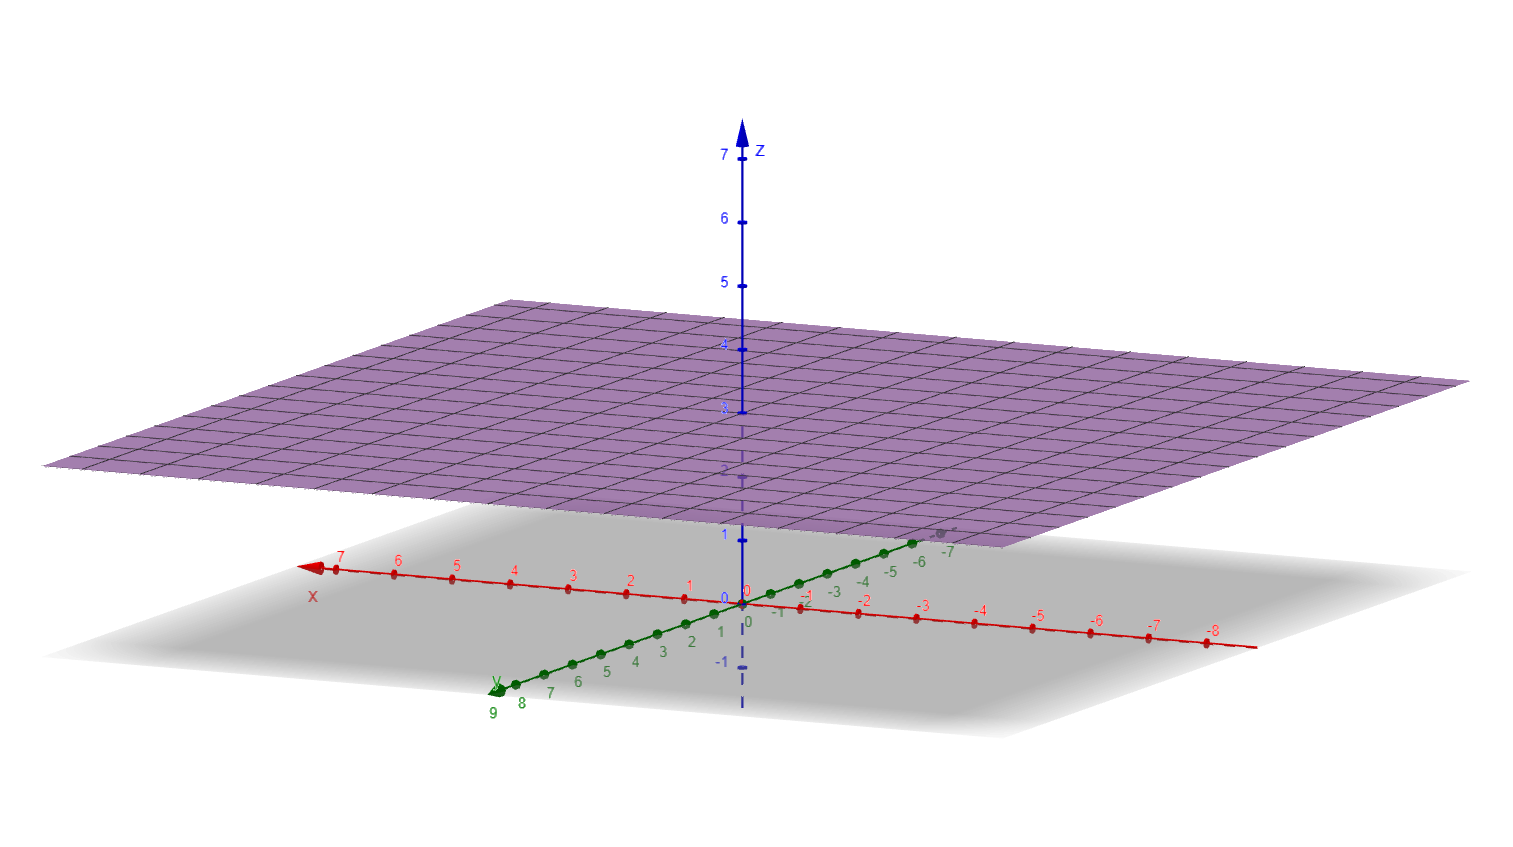
\includegraphics[width = 0.4\textwidth]{Gráfico de f(x,y) = 3.png}               
            \caption{Gráfico de \(f(x,y) = 3\)}
            \label{fig:grafico3}
        \end{figure}
\end{example}

\begin{example}[Função linear]
    Esboce o \href{https://www.geogebra.org/classic/zvdw5ck4}{gráfico} da função afim \[f(x,y) = 6 - 3x - 2y.\]

    Temos que \(D_f = \R^2\) e \(\operatorname{Im}_f = \{z = 6 - 3x - 2y : (x,y)\in\R^2 \}\). 
    
    O gráfico de \(f\) é a superfície \(S\) de equação \(3x + 2y + z = 6\). No 1º octante,
        \begin{itemize}
            \item se \(x=0\), temos a reta \(2y + z = 6\) no plano yz,
            \item se \(y = 0\), temos a reta \(3x + z = 6\) no plano \(xz\), e
            \item se \(z = 0\), temos a reta \(3x + 2y = 6\) no plano \(xy\).
        \end{itemize}
        \begin{figure}[htbp]
            \centering
            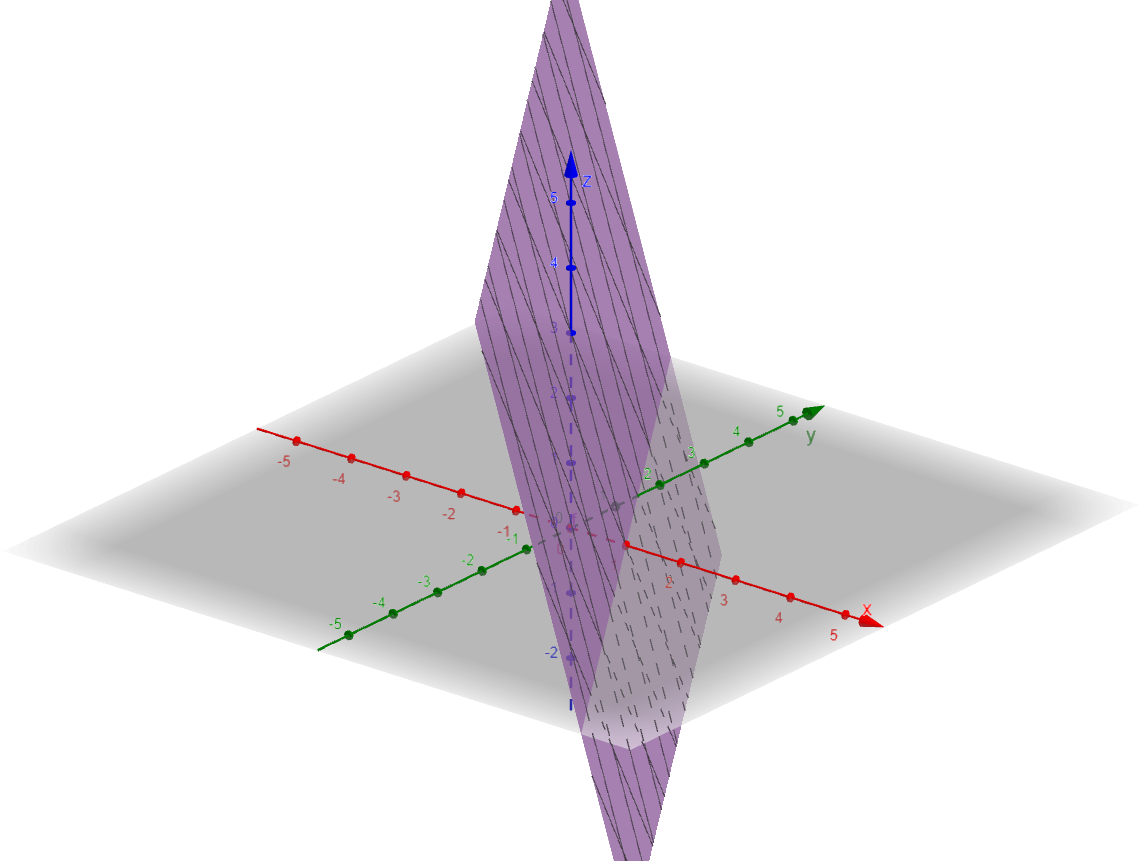
\includegraphics[width=0.7\textwidth]{Gráfico de f(x,y) = 6 - 3x - 2y.png}               
            \caption{Gráfico de \(f(x,y) = 6 -3x - 2y\)}
            \label{fig:grafico4}
        \end{figure}

    Formalmente, sabemos que a equação \(3x + 2y + z = 6\) representa o plano que passa pelo ponto \((0,0,6)\) e é normal ao vetor \(\eta = (3,2,1)\). Ou seja, \[(3,2,1)\cdot[(x,y,z)-(0,0,6)] = 0,\; \forall(x,y,z)\in P.\]
    
    \begin{remark}
    Em geral, o gráfico de uma função afim \(f(x,y) = ax + by + c\) é dado pela equação \[z = ax + by + x \text{ ou } ax + by - z = c\] que é o plano que passa pelo ponto \((0,0,c)\) e é normal ao vetor \(\eta = (a,b,-1)\).
\end{remark}
\end{example}

\begin{example}[Semiesfera]
    Esboce o \href{https://www.geogebra.org/m/jepwjjhe}{gráfico} de \(g(x,y) = \sqrt{9 - x^2 - y^2}\).

    Já vimos que \(D_g = \{(x,y)\in\R^2 : x^2 + y^2 \leq 9 \} \) e \(\operatorname{Im}_g = [0,3]\). Assim, o gráfico de \(g\) tem equação \[z = \sqrt{9 -x^2 - y^2}\] ou ainda \[z^2 = 9 - x^2 - y^2 \Leftrightarrow x^2 + y^2 + z^2 = 3^2.\]
    \begin{figure}[htbp]
        \centering
        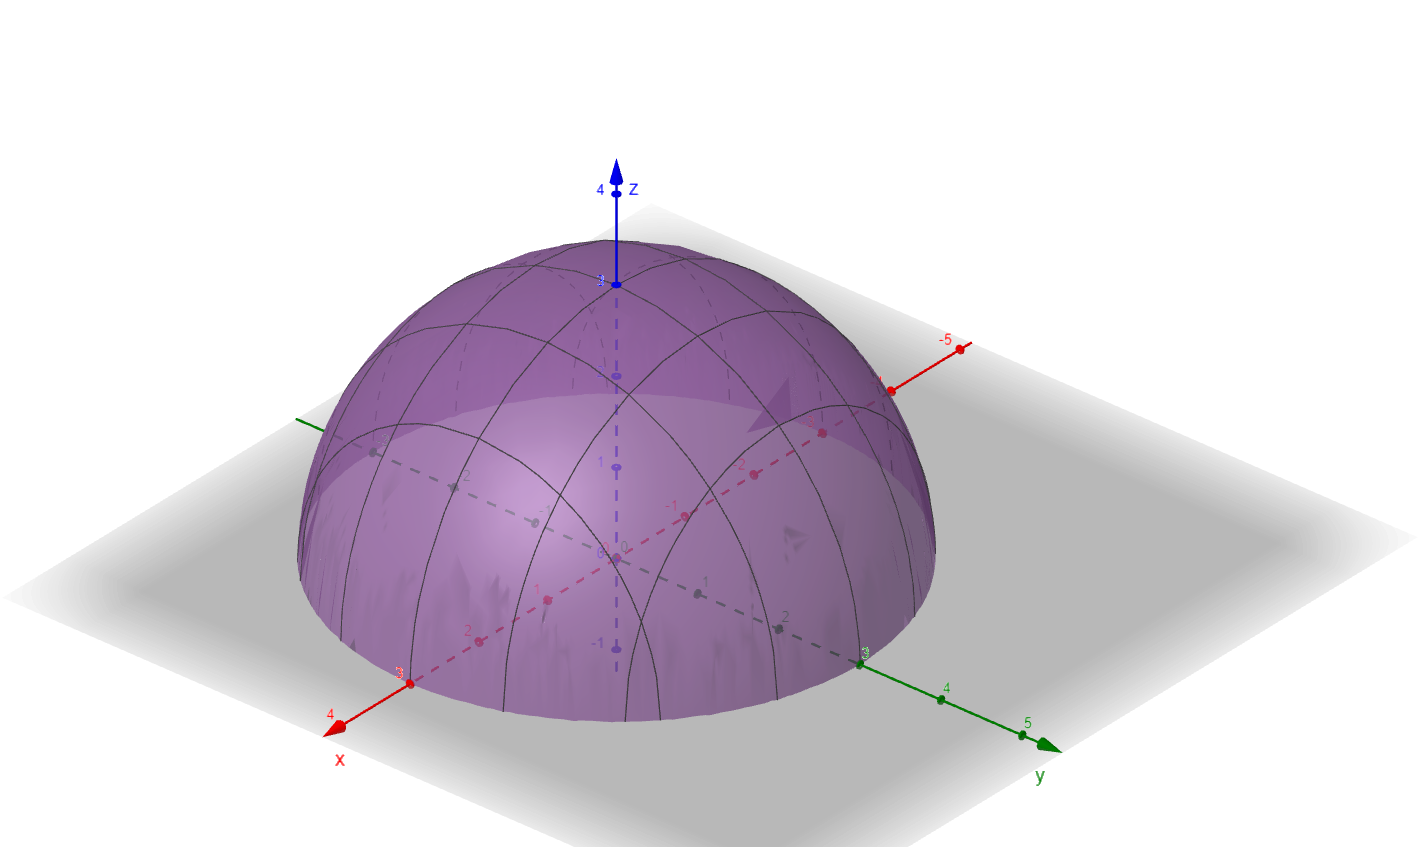
\includegraphics[width=0.75\textwidth]{Gráfico de f(x,y) = sqrt(9-x^2-y^2).png}               
        \caption{Gráfico de \(f(x,y) = \sqrt{9-x^2-y^2}\)}
        \label{fig:grafico5}
    \end{figure}

    Observe que o gráfico de \(g\) é só a metade superior da esfera uma vez que \(z\geq 0\).

    \textbf{Pergunta: } A esfera inteira pode ser representada por uma função de \(x\) e \(y\)?

    Lembre que uma esfera é o conjunto de todos os pontos que possuem a mesma distância de um certo ponto \(\mathcal{O}\). Se \(\mathcal{O} = (a,b,c)\), a equação da esfera de raio \(r\) e centro \(\mathcal{O}\) é o conjunto de todo \((x,y,z)\) tal que \[\|(x,y,z) - (a,b,c)\| = r,\] ou seja \[\sqrt{(x-a)^2 + (y-b)^2 + (z-c)^2} = r,\] ou ainda \[(x-a)^2 + (y-b)^2 + (z-c)^2 = r^2.\] Em particular, se \(\mathcal{O} = (0,0,0)\), então a equação fica \[x^2 + y^2 + z^2 = r^2.\]
\end{example}

\begin{example}[Parabolóide]
    Esboce o \href{https://www.geogebra.org/3d/zhbmek6q}{gráfico} de \(f(x,y) = x^2 + y^2\).

    Temos que \(D_f = \R^2\) e \[\operatorname{Im}_f = \{z = x^2 + y^2 : (x,y)\in\R^2\} = [0,\infty).\] O gráfico de \(f\) tem equação \(z = x^2 + y^2\).

    Para esboçar o gráfico de \(f\) notamos que
        \begin{itemize}
            \item se \(x = 0\), então \(z = y^2\), que é uma parábola no plano yz,
            \item se \(y=0\), temos uma parábola \(z = x^2\) no plano xz,
            \item em geral, se \(y = ax\), então \(z = x^2 + (ax)^2 = (1+a^2)x^2\), ou seja, temos uma parábola no plano (ax)z,
            \item se \(z = k\), temos \(x^2 + y^2 = k\), que é uma circunferência centrada na origem de raio \(\sqrt{k}\).
        \end{itemize}
    \begin{figure}[htbp]
        \centering
        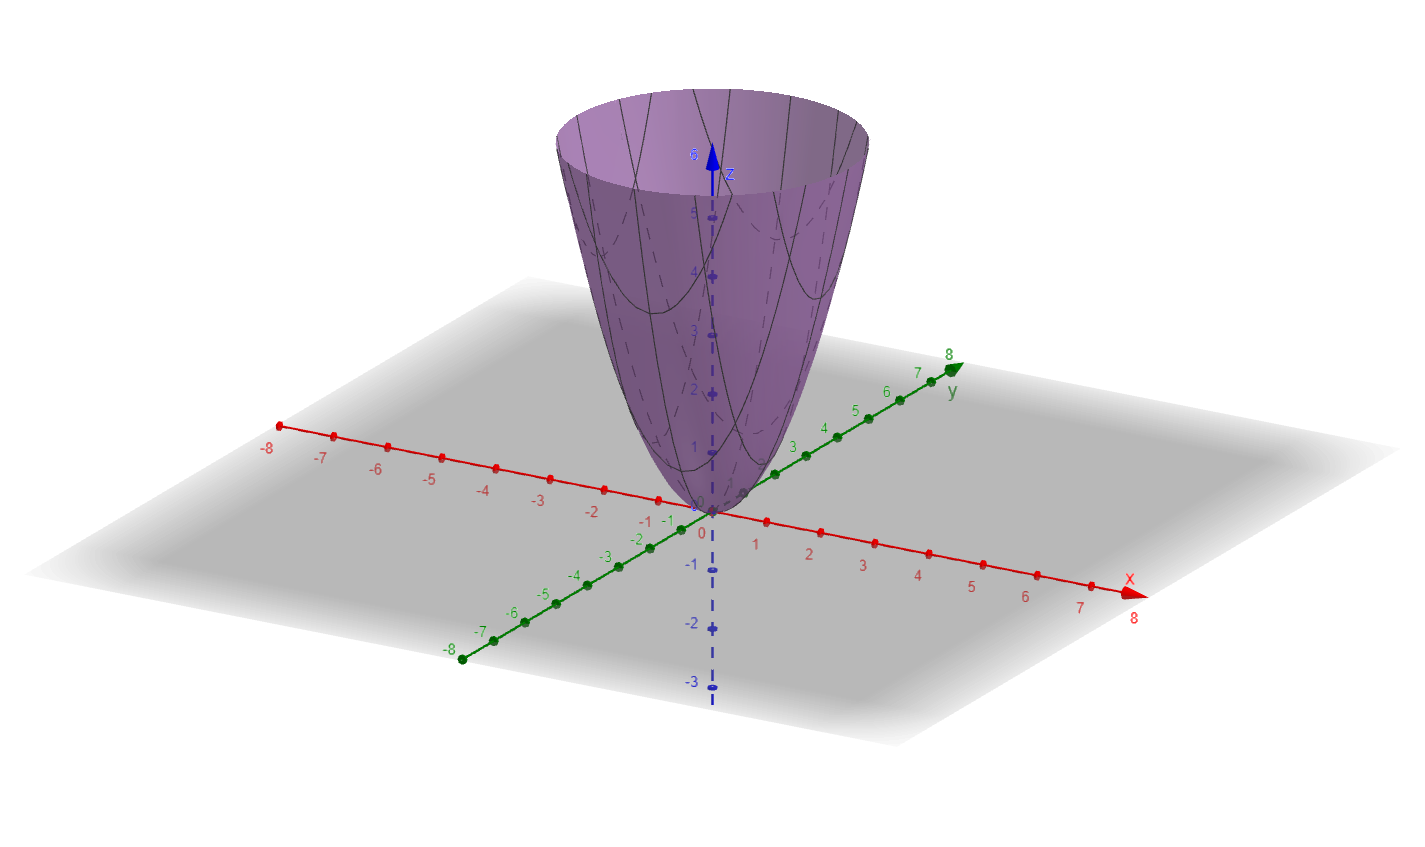
\includegraphics[width=0.7\textwidth]{Gráfico de f(x,y) = x^2 + y^2.png}               
        \caption{Gráfico de \(f(x,y) = x^2 + y^2\)}
        \label{fig:grafico6}
    \end{figure}
\end{example}

\begin{example}[Parabolóide elíptico]
    Esboce o \href{https://www.geogebra.org/3d/j49v7ctq}{gráfico} de \(h(x,y) = 4x^2 + y^2\).

    Temos que \(D_h = \R^2\) e \[\operatorname{Im}_h = \{z = 4x^2 + y^2 : (x,y)\in\R^2\} = [0,\infty].\] O gráfico de \(h\) tem equação \(z = 4x^2 + y^2\).

    Para esboçar o gráfico de \(f\) notamos que
        \begin{itemize}
            \item se \(x = 0\), então \(z = y^2\), que é uma parábola no plano yz,
            \item se \(y=0\), temos uma parábola \(z = 4x^2\) no plano xz,
            \item em geral, se \(y = ax\), então \(z = 4x^2 + (ax)^2 = (4+a^2)x^2\), ou seja, temos uma parábola no plano (ax)z,
            \item se \(z = k\), temos \(4x^2 + y^2 = k\), ou seja \[x^2 + \frac{y^2}{4} = \frac{k}{4} \Leftrightarrow \frac{x^2}{\frac{k}{4}} + \frac{y^2}{k} = 1,\] que são elipses no plano \(z=k\).
        \end{itemize}
    \begin{figure}[htbp]
        \centering
        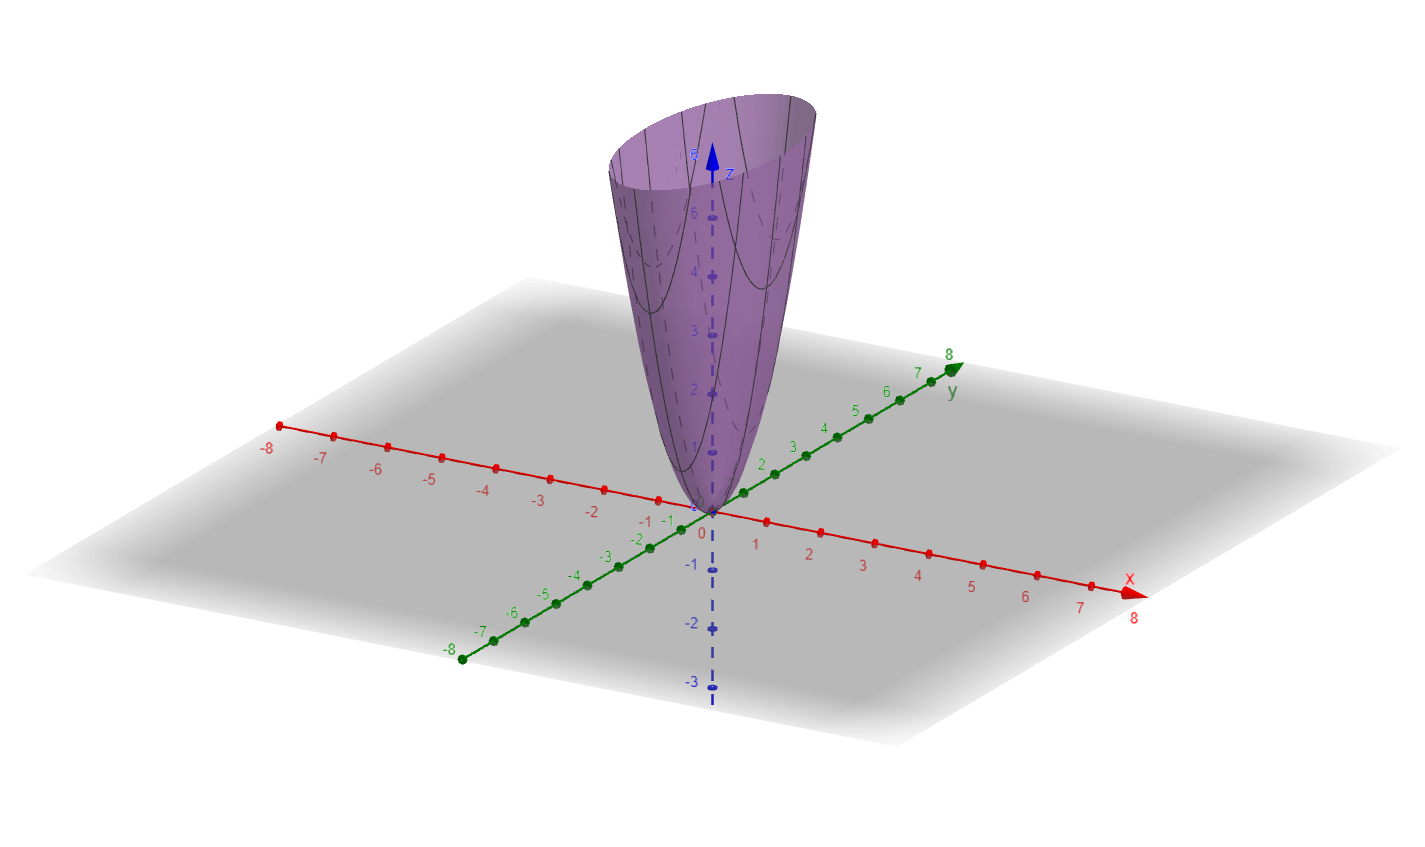
\includegraphics[width=0.7\textwidth]{Gráfico de f(x,y) = 4x^2 + y^2.png}
        \caption{Gráfico de \(f(x,y) = 4x^2 + y^2\)}
        \label{fig:grafico7}
    \end{figure}
\end{example}

Para exemplos de outras superfícies cilíndricas veja \cite[Seção 12.6]{stewart2}.

\begin{example}[Cone]
    Esboce o \href{https://www.geogebra.org/3d/jvjtjdam}{gráfico} da função \(f(x,y) = \sqrt{x^2 + y^2}\).

    Temos que \(D_f = \R^2\) e \(\operatorname{Im}_f = [0,\infty)\) (exercício).

    O gráfico de \(f\) tem equação \(z = \sqrt{x^2 + y^2}\), para esboça-lo notamos que
        \begin{itemize}
            \item se \(x=0\), então \(z = |y|\) no plano yz,
            \item se \(y=0\), temos \(z = |x|\) no plano xz,
            \item se \(z = k\), temos \(x^2 + y^2 = k\), que é uma circunferência no plano \(z=k\) centrada em \((0,0,k)\) e com raio \(\sqrt{k}\), e
            \item se \(y=ax\), então \(z = \sqrt{x^2 + a^2x^2} = |x|\sqrt{1+a^2}\) no plano (ax)z.
        \end{itemize}
    \begin{figure}[htbp]
        \centering
        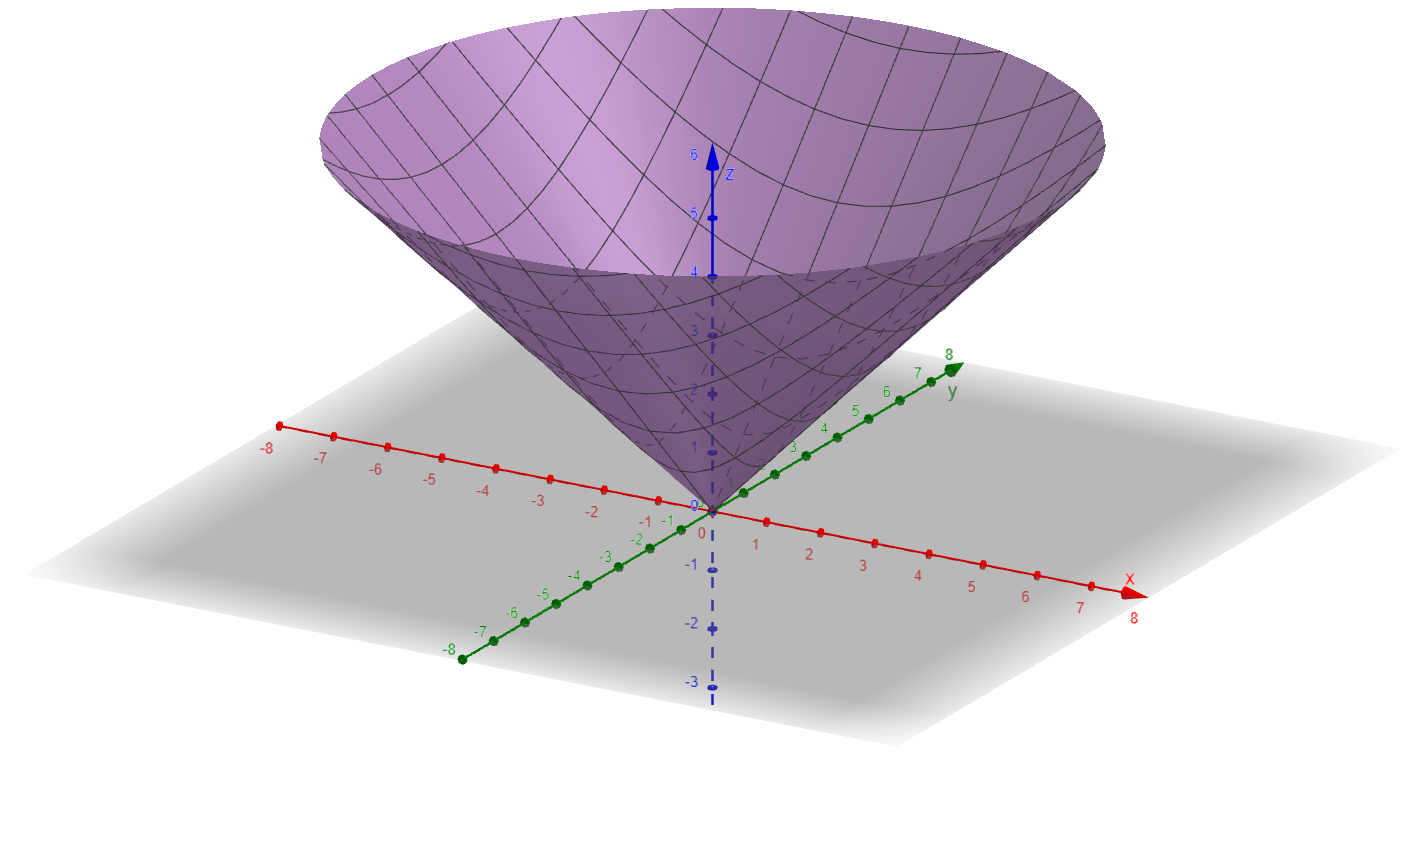
\includegraphics[width=0.6\textwidth]{Gráfico de f(x,y) = sqrt(x^2 + y^2).png}
        \caption{Gráfico de \(f(x,y) = \sqrt{x^2 + y^2}\)}
        \label{fig:grafico9}
    \end{figure}
\end{example}

A representação geométrica do gráfico de uma função de duas variáveis (muitas vezes) pode não ser fácil. Assim, quando queremos ter uma visão geométrica da função podemos usar um método que chamamos de \textbf{curvas de nível}.

\begin{definition}
    Sejam \(z = f(x,y)\) uma função de duas variáveis e \(k\in\operatorname{Im}_f\). O conjunto de todos os pontos \((x,y)\in D_f\) tais que \(f(x,y) = k\) é chamado \textbf{curva de nível}\index{Funções de duas variáveis a valores reais! Curva de nível} de \(f\) correspondente ao nível \(k\).
\end{definition}

% \begin{remark}[Curiosidade]
%     Essa técnica é empregada por cartógrafos nos mapas de contorno em que todos os pontos tem a mesma elevação.
% \end{remark}

Em outras palavras, uma curva de nível \(f(x,y) = k\) mostra, em \(D_f\), onde o gráfico de \(f\) tem altura \(k\).

Ou ainda, as curvas de nível \(f(x,y) = k\) são apenas traços do gráfico de \(f\) no plano horizontal \(z=k\) projetados no plano xy.

Assim, se traçarmos as curvas de nível de uma função e as vizualizamos elevadas para a superfície na altura indicada podemos ``imaginar'' o gráfico da função.
    \begin{figure}[htbp]
        \centering
            \begin{tikzpicture}[x=1.5pt,y=1.5pt,yscale=-1,xscale=1]
                %Straight Lines [id:da9147647358123466] 
                \draw    (81.2,210) -- (81.2,132) ;
                \draw [shift={(81.2,130)}, rotate = 90] [color={rgb, 255:red, 0; green, 0; blue, 0 }  ][line width=0.75]    (6.56,-1.97) .. controls (4.17,-0.84) and (1.99,-0.18) .. (0,0) .. controls (1.99,0.18) and (4.17,0.84) .. (6.56,1.97)   ;
                %Straight Lines [id:da20313754752615065] 
                \draw    (81.2,210) -- (159.2,210) ;
                \draw [shift={(161.2,210)}, rotate = 180] [color={rgb, 255:red, 0; green, 0; blue, 0 }  ][line width=0.75]    (6.56,-1.97) .. controls (4.17,-0.84) and (1.99,-0.18) .. (0,0) .. controls (1.99,0.18) and (4.17,0.84) .. (6.56,1.97)   ;
                %Straight Lines [id:da7849829970447654] 
                \draw    (81.2,210) -- (33.15,249.27) ;
                \draw [shift={(31.6,250.53)}, rotate = 320.74] [color={rgb, 255:red, 0; green, 0; blue, 0 }  ][line width=0.75]    (6.56,-1.97) .. controls (4.17,-0.84) and (1.99,-0.18) .. (0,0) .. controls (1.99,0.18) and (4.17,0.84) .. (6.56,1.97)   ;
                %Shape: Ellipse [id:dp30921184918795663] 
                \draw  [color={rgb, 255:red, 74; green, 144; blue, 226 }  ,draw opacity=1 ] (77.68,230.15) .. controls (77.68,222.85) and (92.82,216.93) .. (111.51,216.93) .. controls (130.19,216.93) and (145.33,222.85) .. (145.33,230.15) .. controls (145.33,237.45) and (130.19,243.37) .. (111.51,243.37) .. controls (92.82,243.37) and (77.68,237.45) .. (77.68,230.15) -- cycle ;
                %Shape: Ellipse [id:dp6534226329652462] 
                \draw  [color={rgb, 255:red, 26; green, 119; blue, 218 }  ,draw opacity=1 ] (82.64,230.15) .. controls (82.64,223.92) and (95.57,218.87) .. (111.51,218.87) .. controls (127.45,218.87) and (140.37,223.92) .. (140.37,230.15) .. controls (140.37,236.38) and (127.45,241.43) .. (111.51,241.43) .. controls (95.57,241.43) and (82.64,236.38) .. (82.64,230.15) -- cycle ;
                %Shape: Ellipse [id:dp2882768010827349] 
                \draw  [color={rgb, 255:red, 0; green, 117; blue, 255 }  ,draw opacity=1 ](91.04,230.15) .. controls (91.04,225.74) and (100.21,222.16) .. (111.51,222.16) .. controls (122.81,222.16) and (131.97,225.74) .. (131.97,230.15) .. controls (131.97,234.57) and (122.81,238.15) .. (111.51,238.15) .. controls (100.21,238.15) and (91.04,234.57) .. (91.04,230.15) -- cycle ;
                %Curve Lines [id:da41599646032066706] 
                \draw [color={rgb, 255:red, 104; green, 175; blue, 255 }  ,draw opacity=1 ][fill={rgb, 255:red, 74; green, 144; blue, 226 }  ,fill opacity=0.29 ]   (77.68,180.24) .. controls (104.48,100.24) and (147.68,164.64) .. (145.68,180.64) .. controls (143.68,196.64) and (81.28,199.44) .. (77.68,180.24) -- cycle ;

                % Text Node
                \draw (18,242.08) node [anchor=north west][inner sep=0.75pt]    {$x$};
                % Text Node
                \draw (167.2,200.48) node [anchor=north west][inner sep=0.75pt]    {$y$};
                % Text Node
                \draw (76,111.48) node [anchor=north west][inner sep=0.75pt]    {$z$};
            \end{tikzpicture}
        \caption{Curvas de nível}
        \label{fig:curvasdenivel}
    \end{figure}

\begin{example}
    Esboce o gráfico e as curvas de nível da função \(f(x,y) = 6 -3x - 2y\) para \(k=0,2,4\) e \(6\).

    Sabemos que \(D_f = \R^2\) e \(\operatorname{Im}_f = \R\), portanto as curvas de nível estão bem definidas para quaisquer \(k\in\R\).
        \begin{itemize}
            \item \(k = 0\): \(f(x,y) = 0 \Leftrightarrow 6 - 3x - 2y = 0 \Leftrightarrow 3x + 2y = 6 \Leftrightarrow y = \frac{6 - 3x}{2}\).
            \item \(k = 2\): \(f(x,y) = 2 \Leftrightarrow 6 - 3x - 2y = 2 \Leftrightarrow 3x + 2y = 4 \Leftrightarrow y = \frac{4 - 3x}{2}\).
            \item \(k = 4\): \(f(x,y) = 4 \Leftrightarrow 6 - 3x - 2y = 4 \Leftrightarrow 3x + 2y = 2 \Leftrightarrow y = \frac{2 - 3x}{2}\).
            \item \(k = 6\): \(f(x,y) = 6 \Leftrightarrow 6 - 3x - 2y = 6 \Leftrightarrow 3x + 2y = 0 \Leftrightarrow y = \frac{-3x}{2}\).
        \end{itemize}

        \begin{figure}[htbp]
            \centering
                \begin{tikzpicture}[x=1.25pt,y=1.25pt,yscale=-1,xscale=1]
    %uncomment if require: \path (0,300); %set diagram left start at 0, and has height of 300
                    %Straight Lines [id:da8990723361816482] 
                    \draw    (192,208.67) -- (192,90.67) ;
                    \draw [shift={(192,88.67)}, rotate = 90] [color={rgb, 255:red, 0; green, 0; blue, 0 }  ][line width=0.75]    (4.37,-1.32) .. controls (2.78,-0.56) and (1.32,-0.12) .. (0,0) .. controls (1.32,0.12) and (2.78,0.56) .. (4.37,1.32)   ;
                    %Straight Lines [id:da7478280448104192] 
                    \draw    (172,188.67) -- (290,188.67) ;
                    \draw [shift={(292,188.67)}, rotate = 180] [color={rgb, 255:red, 0; green, 0; blue, 0 }  ][line width=0.75]    (4.37,-1.32) .. controls (2.78,-0.56) and (1.32,-0.12) .. (0,0) .. controls (1.32,0.12) and (2.78,0.56) .. (4.37,1.32)   ;
                    %Straight Lines [id:da28676267425737956] 
                    \draw [color={rgb, 255:red, 208; green, 2; blue, 27 }  ,draw opacity=1 ]   (153,118.67) -- (203,208.67) ;
                    %Straight Lines [id:da7277707905157709] 
                    \draw [color={rgb, 255:red, 245; green, 166; blue, 35 }  ,draw opacity=1 ]   (166.67,112.67) -- (216.67,202.67) ;
                    %Straight Lines [id:da7275591847875857] 
                    \draw [color={rgb, 255:red, 126; green, 211; blue, 33 }  ,draw opacity=1 ]   (178,103.67) -- (228,193.67) ;
                    %Straight Lines [id:da8404566915602824] 
                    \draw [color={rgb, 255:red, 189; green, 16; blue, 224 }  ,draw opacity=1 ]   (188.33,91) -- (245.18,193.32) ;
                    %Straight Lines [id:da20264971918684138] 
                    \draw    (428.8,191.9) -- (428.67,93.67) ;
                    \draw [shift={(428.67,91.67)}, rotate = 89.92] [color={rgb, 255:red, 0; green, 0; blue, 0 }  ][line width=0.75]    (4.37,-1.32) .. controls (2.78,-0.56) and (1.32,-0.12) .. (0,0) .. controls (1.32,0.12) and (2.78,0.56) .. (4.37,1.32)   ;
                    %Straight Lines [id:da3198102385142041] 
                    \draw    (428.8,191.9) -- (526.67,191.67) ;
                    \draw [shift={(528.67,191.67)}, rotate = 179.87] [color={rgb, 255:red, 0; green, 0; blue, 0 }  ][line width=0.75]    (4.37,-1.32) .. controls (2.78,-0.56) and (1.32,-0.12) .. (0,0) .. controls (1.32,0.12) and (2.78,0.56) .. (4.37,1.32)   ;
                    %Straight Lines [id:da9181883297393563] 
                    \draw    (428.8,191.9) -- (387.21,233.81) ;
                    \draw [shift={(385.8,235.23)}, rotate = 314.78] [color={rgb, 255:red, 0; green, 0; blue, 0 }  ][line width=0.75]    (4.37,-1.32) .. controls (2.78,-0.56) and (1.32,-0.12) .. (0,0) .. controls (1.32,0.12) and (2.78,0.56) .. (4.37,1.32)   ;
                    %Straight Lines [id:da5374149032464713] 
                    \draw [draw opacity=0][fill={rgb, 255:red, 74; green, 144; blue, 226 }  ,fill opacity=0.36 ]   (428.47,112.57) -- (407.3,213.57) -- (488.8,191.9) -- cycle ;
                    %Straight Lines [id:da6924013277673103] 
                    \draw [color={rgb, 255:red, 189; green, 16; blue, 224 }  ,draw opacity=1 ]   (407.3,213.57) -- (488.8,191.9) ;
                    %Straight Lines [id:da8716167998681623] 
                    \draw [color={rgb, 255:red, 126; green, 211; blue, 33 }  ,draw opacity=1 ]   (412.47,187.9) -- (473.13,170.9) ;
                    %Straight Lines [id:da7369820628309036] 
                    \draw [color={rgb, 255:red, 245; green, 166; blue, 35 }  ,draw opacity=1 ]   (420.13,153.23) -- (453.8,145.23) ;
                    %Straight Lines [id:da7423607072321098] 
                    \draw [color={rgb, 255:red, 208; green, 2; blue, 27 }  ,draw opacity=1 ]   (426.8,113.23) -- (431.13,112.9) ;

                    % Text Node
                    \draw (296.4,181.67) node [anchor=north west][inner sep=0.75pt]  [font=\normalsize]  {$x$};
                    % Text Node
                    \draw (186.4,72.13) node [anchor=north west][inner sep=0.75pt]  [font=\normalsize]  {$y$};
                    % Text Node
                    \draw (194,212.07) node [anchor=north west][inner sep=0.75pt]  [font=\normalsize]  {$\textcolor[rgb]{0.82,0.01,0.11}{k=6}$};
                    % Text Node
                    \draw (218.67,206.07) node [anchor=north west][inner sep=0.75pt]  [font=\normalsize,color={rgb, 255:red, 245; green, 166; blue, 35 }  ,opacity=1 ]  {$\textcolor[rgb]{0.96,0.65,0.14}{k=4}$};
                    % Text Node
                    \draw (230,197.07) node [anchor=north west][inner sep=0.75pt]  [font=\normalsize,color={rgb, 255:red, 245; green, 166; blue, 35 }  ,opacity=1 ]  {$\textcolor[rgb]{0.49,0.83,0.13}{k=2}$};
                    % Text Node
                    \draw (243.56,176.88) node [anchor=north west][inner sep=0.75pt]  [font=\normalsize,color={rgb, 255:red, 245; green, 166; blue, 35 }  ,opacity=1 ]  {$\textcolor[rgb]{0.74,0.06,0.88}{k=0}$};
                    % Text Node
                    \draw (533.07,184.67) node [anchor=north west][inner sep=0.75pt]  [font=\normalsize]  {$x$};
                    % Text Node
                    \draw (423.07,75.13) node [anchor=north west][inner sep=0.75pt]  [font=\normalsize]  {$y$};
                    % Text Node
                    \draw (490.8,195.3) node [anchor=north west][inner sep=0.75pt]  [font=\normalsize,color={rgb, 255:red, 245; green, 166; blue, 35 }  ,opacity=1 ]  {$\textcolor[rgb]{0.74,0.06,0.88}{k=0}$};
                    % Text Node
                    \draw (474.17,163.3) node [anchor=north west][inner sep=0.75pt]  [font=\normalsize,color={rgb, 255:red, 245; green, 166; blue, 35 }  ,opacity=1 ]  {$\textcolor[rgb]{0.49,0.83,0.13}{k=2}$};
                    % Text Node
                    \draw (453.51,137.97) node [anchor=north west][inner sep=0.75pt]  [font=\normalsize,color={rgb, 255:red, 245; green, 166; blue, 35 }  ,opacity=1 ]  {$\textcolor[rgb]{0.96,0.65,0.14}{k=4}$};
                    % Text Node
                    \draw (432.27,105.3) node [anchor=north west][inner sep=0.75pt]  [font=\normalsize,color={rgb, 255:red, 245; green, 166; blue, 35 }  ,opacity=1 ]  {$\textcolor[rgb]{0.82,0.01,0.11}{k=6}$};
                \end{tikzpicture}
            \caption{Curvas de nível e gráfico da função \(f(x,y) = 6 - 3x - 2y\).}
            \label{fig:curvasdenivel1}
        \end{figure}
\end{example}

\begin{example}
    Esboce o gráfico e as curvas de nível da função \(g(x,y) = \sqrt{9 - x^2 - y^2}\) para \(k=0,1,2\) e \(3\).

    Sabemos que \(D_f = \{(x,y)\in\R^2 : x^2 + y^2 \leq 9\}\) e \(\operatorname{Im}_f = [0,3]\), portanto as curvas de nível está bem definidas para \(k\in[0,3]\).
    \begin{itemize}
            \item \(k = 0\): \(g(x,y) = 0 \Rightarrow \sqrt{9 - x^2 - y^2} = 0 \Rightarrow x^2 + y^2 = 9\)
            \item \(k = 1\): \(g(x,y) = 1 \Rightarrow \sqrt{9 - x^2 - y^2} = 1 \Rightarrow x^2 + y^2 = 8\)
            \item \(k = 2\): \(g(x,y) = 0 \Rightarrow \sqrt{9 - x^2 - y^2} = 2 \Rightarrow x^2 + y^2 = 5\)
            \item \(k = 3\): \(g(x,y) = 0 \Rightarrow \sqrt{9 - x^2 - y^2} = 3 \Rightarrow x^2 + y^2 = 0\)
        \end{itemize}
        \begin{figure}[htbp]
            \centering
                \begin{tikzpicture}[x=1.25pt,y=1.25pt,yscale=-1,xscale=1]
    %uncomment if require: \path (0,300); %set diagram left start at 0, and has height of 300
                    %Straight Lines [id:da9005421899192951] 
                    \draw    (200,229.8) -- (200,111.8) ;
                    \draw [shift={(200,109.8)}, rotate = 90] [color={rgb, 255:red, 0; green, 0; blue, 0 }  ][line width=0.75]    (4.37,-1.32) .. controls (2.78,-0.56) and (1.32,-0.12) .. (0,0) .. controls (1.32,0.12) and (2.78,0.56) .. (4.37,1.32)   ;
                    %Straight Lines [id:da22363777483293845] 
                    \draw    (144,179.4) -- (262,179.4) ;
                    \draw [shift={(264,179.4)}, rotate = 180] [color={rgb, 255:red, 0; green, 0; blue, 0 }  ][line width=0.75]    (4.37,-1.32) .. controls (2.78,-0.56) and (1.32,-0.12) .. (0,0) .. controls (1.32,0.12) and (2.78,0.56) .. (4.37,1.32)   ;
                    %Straight Lines [id:da08360455299313296] 
                    \draw    (400.8,180.3) -- (400.67,82.07) ;
                    \draw [shift={(400.67,80.07)}, rotate = 89.92] [color={rgb, 255:red, 0; green, 0; blue, 0 }  ][line width=0.75]    (4.37,-1.32) .. controls (2.78,-0.56) and (1.32,-0.12) .. (0,0) .. controls (1.32,0.12) and (2.78,0.56) .. (4.37,1.32)   ;
                    %Straight Lines [id:da1255686424003376] 
                    \draw    (400.8,180.3) -- (498.67,180.07) ;
                    \draw [shift={(500.67,180.07)}, rotate = 179.87] [color={rgb, 255:red, 0; green, 0; blue, 0 }  ][line width=0.75]    (4.37,-1.32) .. controls (2.78,-0.56) and (1.32,-0.12) .. (0,0) .. controls (1.32,0.12) and (2.78,0.56) .. (4.37,1.32)   ;
                    %Straight Lines [id:da9713829965193167] 
                    \draw    (400.8,180.3) -- (359.21,222.21) ;
                    \draw [shift={(357.8,223.63)}, rotate = 314.78] [color={rgb, 255:red, 0; green, 0; blue, 0 }  ][line width=0.75]    (4.37,-1.32) .. controls (2.78,-0.56) and (1.32,-0.12) .. (0,0) .. controls (1.32,0.12) and (2.78,0.56) .. (4.37,1.32)   ;
                    %Shape: Circle [id:dp6116890534445036] 
                    \draw  [draw opacity=0][fill={rgb, 255:red, 189; green, 16; blue, 224 }  ,fill opacity=1 ] (198.02,179.37) .. controls (198.02,178.22) and (198.95,177.29) .. (200.1,177.29) .. controls (201.25,177.29) and (202.18,178.22) .. (202.18,179.37) .. controls (202.18,180.52) and (201.25,181.45) .. (200.1,181.45) .. controls (198.95,181.45) and (198.02,180.52) .. (198.02,179.37) -- cycle ;
                    %Shape: Circle [id:dp019052448495683993] 
                    \draw  [color={rgb, 255:red, 126; green, 211; blue, 33 }  ,draw opacity=1 ] (179.97,179.37) .. controls (179.97,168.26) and (188.99,159.25) .. (200.1,159.25) .. controls (211.21,159.25) and (220.22,168.26) .. (220.22,179.37) .. controls (220.22,190.48) and (211.21,199.5) .. (200.1,199.5) .. controls (188.99,199.5) and (179.97,190.48) .. (179.97,179.37) -- cycle ;
                    %Shape: Circle [id:dp517180935046544] 
                    \draw  [color={rgb, 255:red, 208; green, 2; blue, 27 }  ,draw opacity=1 ] (170.24,179.37) .. controls (170.24,162.88) and (183.61,149.52) .. (200.1,149.52) .. controls (216.59,149.52) and (229.95,162.88) .. (229.95,179.37) .. controls (229.95,195.86) and (216.59,209.22) .. (200.1,209.22) .. controls (183.61,209.22) and (170.24,195.86) .. (170.24,179.37) -- cycle ;
                    %Shape: Circle [id:dp6339164611040847] 
                    \draw  [color={rgb, 255:red, 74; green, 144; blue, 226 }  ,draw opacity=1 ] (159.82,179.37) .. controls (159.82,157.12) and (177.85,139.09) .. (200.1,139.09) .. controls (222.35,139.09) and (240.38,157.12) .. (240.38,179.37) .. controls (240.38,201.62) and (222.35,219.65) .. (200.1,219.65) .. controls (177.85,219.65) and (159.82,201.62) .. (159.82,179.37) -- cycle ;
                    %Flowchart: Connector [id:dp6414617703668187] 
                    \draw  [draw opacity=0][fill={rgb, 255:red, 245; green, 166; blue, 35 }  ,fill opacity=0.51 ] (369.04,179.88) .. controls (369.04,173.3) and (383.47,167.97) .. (401.26,167.97) .. controls (419.06,167.97) and (433.49,173.3) .. (433.49,179.88) .. controls (433.49,186.45) and (419.06,191.79) .. (401.26,191.79) .. controls (383.47,191.79) and (369.04,186.45) .. (369.04,179.88) -- cycle ;
                    %Shape: Chord [id:dp6504135876557121] 
                    \draw  [draw opacity=0][fill={rgb, 255:red, 245; green, 166; blue, 35 }  ,fill opacity=0.46 ] (369.04,179.88) .. controls (367.25,176.27) and (366.26,172.31) .. (366.26,168.15) .. controls (366.26,151.58) and (381.93,138.15) .. (401.26,138.15) .. controls (420.59,138.15) and (436.26,151.58) .. (436.26,168.15) .. controls (436.26,172.38) and (435.24,176.41) .. (433.4,180.06) -- cycle ;
                    %Flowchart: Connector [id:dp925863392347943] 
                    \draw  [color={rgb, 255:red, 74; green, 144; blue, 226 }  ,draw opacity=1 ] (368.58,180.3) .. controls (368.58,173.72) and (383,168.39) .. (400.8,168.39) .. controls (418.6,168.39) and (433.02,173.72) .. (433.02,180.3) .. controls (433.02,186.88) and (418.6,192.21) .. (400.8,192.21) .. controls (383,192.21) and (368.58,186.88) .. (368.58,180.3) -- cycle ;
                    %Flowchart: Connector [id:dp05038336129863108] 
                    \draw  [color={rgb, 255:red, 208; green, 2; blue, 27 }  ,draw opacity=1 ] (366.08,168.8) .. controls (366.08,162.22) and (381.82,156.89) .. (401.24,156.89) .. controls (420.66,156.89) and (436.4,162.22) .. (436.4,168.8) .. controls (436.4,175.38) and (420.66,180.71) .. (401.24,180.71) .. controls (381.82,180.71) and (366.08,175.38) .. (366.08,168.8) -- cycle ;
                    %Flowchart: Connector [id:dp616582824034949] 
                    \draw  [color={rgb, 255:red, 126; green, 211; blue, 33 }  ,draw opacity=1 ] (371.08,154.8) .. controls (371.08,148.22) and (384.69,142.89) .. (401.49,142.89) .. controls (418.28,142.89) and (431.9,148.22) .. (431.9,154.8) .. controls (431.9,161.38) and (418.28,166.71) .. (401.49,166.71) .. controls (384.69,166.71) and (371.08,161.38) .. (371.08,154.8) -- cycle ;
                    %Shape: Circle [id:dp8982011313141853] 
                    \draw  [draw opacity=0][fill={rgb, 255:red, 189; green, 16; blue, 224 }  ,fill opacity=1 ] (399.02,138.37) .. controls (399.02,137.22) and (399.95,136.29) .. (401.1,136.29) .. controls (402.25,136.29) and (403.18,137.22) .. (403.18,138.37) .. controls (403.18,139.52) and (402.25,140.45) .. (401.1,140.45) .. controls (399.95,140.45) and (399.02,139.52) .. (399.02,138.37) -- cycle ;

                    % Text Node
                    \draw (269.6,174.8) node [anchor=north west][inner sep=0.75pt]  [font=\normalsize]  {$x$};
                    % Text Node
                    \draw (194,95.27) node [anchor=north west][inner sep=0.75pt]  [font=\normalsize]  {$y$};
                    % Text Node
                    \draw (344.4,218.4) node [anchor=north west][inner sep=0.75pt]  [font=\normalsize]  {$x$};
                    % Text Node
                    \draw (395.07,63.53) node [anchor=north west][inner sep=0.75pt]  [font=\normalsize]  {$z$};
                    % Text Node
                    \draw (193.7,183.85) node [anchor=north west][inner sep=0.75pt]  [font=\normalsize]  {$\textcolor[rgb]{0.74,0.06,0.88}{k=3}$};
                    % Text Node
                    \draw (193.2,165.8) node [anchor=north west][inner sep=0.75pt]  [font=\normalsize]  {$\textcolor[rgb]{0.49,0.83,0.13}{k=2}$};
                    % Text Node
                    \draw (193.45,153.5) node [anchor=north west][inner sep=0.75pt]  [font=\normalsize]  {$\textcolor[rgb]{0.82,0.01,0.11}{k=1}$};
                    % Text Node
                    \draw (190.95,142) node [anchor=north west][inner sep=0.75pt]  [font=\normalsize]  {$\textcolor[rgb]{0.29,0.56,0.89}{k=0}$};
                    % Text Node
                    \draw (504.53,170.53) node [anchor=north west][inner sep=0.75pt]    {$y$};

                \end{tikzpicture}
            \caption{Curvas de nível e gráfico da função \(f(x,y) = \sqrt{9-x^2-y^2}\).}
            \label{fig:curvasdenivel2}
        \end{figure}
\end{example}

\begin{example}
    Seja \(f(x,y) = \frac{1}{x^2 + y^2}\). Determine o domínio e a imagem de \(f\). Em seguida esboce suas curvas de nível e gráfico.

    É claro que \(D_f = \{(x,y)\in\R^2 : (x,y)\neq (0,0)\}\) e \[\operatorname{Im}_f = \{z=f(x,y) : (x,y)\in D_f\} = \left\{ x = \frac{1}{x^2 + y^2} : (x,y)\neq(0,0) \right\} = (0,\infty).\] Além disso, para \(k>0\) temos \[\frac{1}{x^2 + y^2} = k \Rightarrow x^2 + y^2 = \frac{1}{k},\] portanto as curvas de nível são circunferências concêntricas de raio \(\sqrt{\frac{1}{k}}\). Observe que quando \(k\) é pequeno, o raio da circunferência é grande, e quando \(k\) é grande, o raio é pequeno. Além disso, note que, se \(x=0\), então \(z = \frac{1}{y^2}\) é uma hiperbole no plano yz; agora se \(y=0\), \(z = \frac{1}{x^2}\) é uma hiperbole no plano xz. Com essas informações podemos esboçar as curvas de nível e o gráfico de \(f\).
\begin{figure}[htbp]
            \centering
                \begin{tikzpicture}[x=1.25pt,y=1.25pt,yscale=-1,xscale=1]
    %uncomment if require: \path (0,300); %set diagram left start at 0, and has height of 300
                    %Straight Lines [id:da24437428975701714] 
                    \draw    (80.67,206.8) -- (80.67,88.8) ;
                    \draw [shift={(80.67,86.8)}, rotate = 90] [color={rgb, 255:red, 0; green, 0; blue, 0 }  ][line width=0.75]    (4.37,-1.32) .. controls (2.78,-0.56) and (1.32,-0.12) .. (0,0) .. controls (1.32,0.12) and (2.78,0.56) .. (4.37,1.32)   ;
                    %Straight Lines [id:da10202597957111392] 
                    \draw    (24.67,156.4) -- (142.67,156.4) ;
                    \draw [shift={(144.67,156.4)}, rotate = 180] [color={rgb, 255:red, 0; green, 0; blue, 0 }  ][line width=0.75]    (4.37,-1.32) .. controls (2.78,-0.56) and (1.32,-0.12) .. (0,0) .. controls (1.32,0.12) and (2.78,0.56) .. (4.37,1.32)   ;
                    %Straight Lines [id:da03442276412344114] 
                    \draw    (282.13,167.3) -- (282,69.07) ;
                    \draw [shift={(282,67.07)}, rotate = 89.92] [color={rgb, 255:red, 0; green, 0; blue, 0 }  ][line width=0.75]    (4.37,-1.32) .. controls (2.78,-0.56) and (1.32,-0.12) .. (0,0) .. controls (1.32,0.12) and (2.78,0.56) .. (4.37,1.32)   ;
                    %Straight Lines [id:da8565157872425141] 
                    \draw    (282.13,167.3) -- (380,167.07) ;
                    \draw [shift={(382,167.07)}, rotate = 179.87] [color={rgb, 255:red, 0; green, 0; blue, 0 }  ][line width=0.75]    (4.37,-1.32) .. controls (2.78,-0.56) and (1.32,-0.12) .. (0,0) .. controls (1.32,0.12) and (2.78,0.56) .. (4.37,1.32)   ;
                    %Straight Lines [id:da005485083537555058] 
                    \draw    (282.13,167.3) -- (240.54,209.21) ;
                    \draw [shift={(239.13,210.63)}, rotate = 314.78] [color={rgb, 255:red, 0; green, 0; blue, 0 }  ][line width=0.75]    (4.37,-1.32) .. controls (2.78,-0.56) and (1.32,-0.12) .. (0,0) .. controls (1.32,0.12) and (2.78,0.56) .. (4.37,1.32)   ;
                    %Shape: Circle [id:dp8256132701254346] 
                    \draw  [color={rgb, 255:red, 126; green, 211; blue, 33 }  ,draw opacity=1 ] (60.64,156.37) .. controls (60.64,145.26) and (69.65,136.25) .. (80.77,136.25) .. controls (91.88,136.25) and (100.89,145.26) .. (100.89,156.37) .. controls (100.89,167.48) and (91.88,176.5) .. (80.77,176.5) .. controls (69.65,176.5) and (60.64,167.48) .. (60.64,156.37) -- cycle ;
                    %Shape: Circle [id:dp1765127823583098] 
                    \draw  [color={rgb, 255:red, 208; green, 2; blue, 27 }  ,draw opacity=1 ] (50.91,156.37) .. controls (50.91,139.88) and (64.28,126.52) .. (80.77,126.52) .. controls (97.26,126.52) and (110.62,139.88) .. (110.62,156.37) .. controls (110.62,172.86) and (97.26,186.22) .. (80.77,186.22) .. controls (64.28,186.22) and (50.91,172.86) .. (50.91,156.37) -- cycle ;
                    %Shape: Circle [id:dp6534693648452948] 
                    \draw  [color={rgb, 255:red, 74; green, 144; blue, 226 }  ,draw opacity=1 ] (40.49,156.37) .. controls (40.49,134.12) and (58.52,116.09) .. (80.77,116.09) .. controls (103.01,116.09) and (121.05,134.12) .. (121.05,156.37) .. controls (121.05,178.62) and (103.01,196.65) .. (80.77,196.65) .. controls (58.52,196.65) and (40.49,178.62) .. (40.49,156.37) -- cycle ;
                    %Flowchart: Connector [id:dp20357625150336012] 
                    \draw  [color={rgb, 255:red, 208; green, 2; blue, 27 }  ,draw opacity=1 ][fill={rgb, 255:red, 208; green, 2; blue, 27 }  ,fill opacity=0.25 ][dash pattern={on 0.84pt off 2.51pt}] (249.56,146.81) .. controls (249.55,143.58) and (263.93,140.92) .. (281.69,140.88) .. controls (299.44,140.83) and (313.84,143.42) .. (313.85,146.66) .. controls (313.86,149.89) and (299.47,152.55) .. (281.72,152.59) .. controls (263.96,152.64) and (249.57,150.05) .. (249.56,146.81) -- cycle ;
                    %Flowchart: Connector [id:dp728442972792305] 
                    \draw  [color={rgb, 255:red, 74; green, 144; blue, 226 }  ,draw opacity=1 ][fill={rgb, 255:red, 74; green, 144; blue, 226 }  ,fill opacity=0.25 ][dash pattern={on 0.84pt off 2.51pt}] (230.88,175.11) .. controls (230.85,165.57) and (254.01,157.78) .. (282.61,157.71) .. controls (311.2,157.64) and (334.4,165.31) .. (334.42,174.86) .. controls (334.45,184.4) and (311.29,192.19) .. (282.69,192.26) .. controls (254.1,192.33) and (230.9,184.65) .. (230.88,175.11) -- cycle ;
                    %Flowchart: Connector [id:dp8540526439832161] 
                    \draw  [color={rgb, 255:red, 126; green, 211; blue, 33 }  ,draw opacity=1 ][fill={rgb, 255:red, 126; green, 211; blue, 33 }  ,fill opacity=0.25 ][dash pattern={on 0.84pt off 2.51pt}] (261.22,129.95) .. controls (261.22,126.71) and (270.61,124.07) .. (282.21,124.04) .. controls (293.81,124.01) and (303.22,126.61) .. (303.22,129.85) .. controls (303.23,133.08) and (293.84,135.73) .. (282.24,135.76) .. controls (270.64,135.78) and (261.23,133.18) .. (261.22,129.95) -- cycle ;
                    %Flowchart: Connector [id:dp14611648575471736] 
                    \draw  [color={rgb, 255:red, 144; green, 19; blue, 254 }  ,draw opacity=1 ][fill={rgb, 255:red, 189; green, 16; blue, 224 }  ,fill opacity=0.25 ][dash pattern={on 0.84pt off 2.51pt}] (271.77,113.51) .. controls (271.77,111.47) and (276.81,109.8) .. (283.04,109.78) .. controls (289.27,109.77) and (294.33,111.41) .. (294.34,113.46) .. controls (294.34,115.5) and (289.29,117.17) .. (283.06,117.18) .. controls (276.83,117.2) and (271.78,115.55) .. (271.77,113.51) -- cycle ;
                    %Curve Lines [id:da860309563236923] 
                    \draw    (230.88,175.11) .. controls (260.13,132) and (280.13,114.29) .. (278.13,75.43) ;
                    %Curve Lines [id:da9346030576531226] 
                    \draw    (288.42,77.43) .. controls (291.56,126) and (312.99,147.14) .. (333.56,176.29) ;

                    % Text Node
                    \draw (150.27,151.8) node [anchor=north west][inner sep=0.75pt]  [font=\footnotesize]  {$x$};
                    % Text Node
                    \draw (74.67,72.27) node [anchor=north west][inner sep=0.75pt]  [font=\normalsize]  {$y$};
                    % Text Node
                    \draw (227.73,205.4) node [anchor=north west][inner sep=0.75pt]  [font=\normalsize]  {$x$};
                    % Text Node
                    \draw (276.4,50.53) node [anchor=north west][inner sep=0.75pt]  [font=\normalsize]  {$z$};
                    % Text Node
                    \draw (124.15,129.09) node [anchor=north west][inner sep=0.75pt]  [font=\normalsize]  {$\textcolor[rgb]{0.49,0.83,0.13}{k=2}$};
                    % Text Node
                    \draw (124.12,119.36) node [anchor=north west][inner sep=0.75pt]  [font=\normalsize]  {$\textcolor[rgb]{0.82,0.01,0.11}{k=1}$};
                    % Text Node
                    \draw (123.9,96.14) node [anchor=north west][inner sep=0.75pt]  [font=\normalsize]  {$\textcolor[rgb]{0.29,0.56,0.89}{k=\frac{1}{2}}$};
                    % Text Node
                    \draw (385.87,157.53) node [anchor=north west][inner sep=0.75pt]    {$y$};
                \end{tikzpicture}
            \caption{Curvas de nível e gráfico da função \(f(x,y) = \frac{1}{x^2+y^2}\).}
            \label{fig:curvasdenivel3}
        \end{figure}
\end{example}

\begin{exercise}
    \begin{enumerate}
        \item Desenhe as curvas de nível e esboce o gráfico de \(f(x,y) = x^2 + y^2\).
        \item Seja \(f(x,y) = \frac{y}{x-1}\).
            \begin{enumerate}
                \item Determine \(D_f\) e \(\operatorname{Im}_f\).
                \item Desenhe as curvas de nível para \(k = -1,0,1\) e \(2\).
                \item Tente imaginar e esboçar o gráfico de \(f\).
            \end{enumerate}
    \end{enumerate}
\end{exercise}

\section{Funções de 3 variáveis e superfícies de nível}

\begin{definition}\index{Funções de três variáveis reais a valores reais}
    Uma \textbf{função de três variáveis a valores reais}, definida em \(D_f \subset\R^3\), é uma função que associa a cada terna ordenada \((x,y,z)\in D_f\) a um único número real \(w = f(x,y,z)\).
\end{definition}

\begin{definition}\index{Funções de três variáveis reais a valores reais! Gráfico}
    O \textbf{gráfico} de uma função de 3 variáveis é o conjunto \[G_f = \{(x,y,z,w)\in\R^4 : w = f(x,y,z),\, (x,y,z)\in D_f\}.\]
\end{definition}

% Infelizmente não conseguimos nem ao menos imaginar o gráfico de uma função de três variáveis. Para ganharmos um pouco de intuição acerca de seu comportamento, desenhamos suas superfícies de nível.

\begin{definition}\index{Funções de três variáveis reais a valores reais! Superfícies de nível}
    Sejam \(f:D_f\subset\R^3 \to \R\) uma função e \(k\in\operatorname{Im}_f\). O conjunto dos pontos \((x,y,z)\in D_f\) tais que \(f(x,y,z) = k\) é chamado de superfície de nível \(k\) de \(f\).
\end{definition}

Observe que se um ponto se move ao longo de uma superfície de nível, o valor de \(f(x,y,z)\) permanece fixo.

\begin{example}
    Determine as superfícies de nível de \(f(x,y,z) = x^2 + y^2 + z^2\).

    Temos \(D_f = \R^3\) e \[\operatorname{Im}_f = \{ w = x^2 + y^2 + z^2 : (x,y,z)\in\R^3 \} = \{w\geq\} = [0,\infty).\] Portanto, para \(k\geq 0\) temos \[f(x,y,z) = k \Leftrightarrow x^2 + y^2 + z^2 = k,\] ou seja, as superfícies de nível de \(f\) são esferas concêntricas de raio \(\sqrt{k}\) centradas na origem.
        \begin{figure}[htbp]
            \centering
                \begin{tikzpicture}[x=0.5pt,y=0.5pt,yscale=-1,xscale=1]
                    %Straight Lines [id:da14017589294902055] 
                    \draw    (310.62,189.37) -- (421.33,189.37) ;
                    \draw [shift={(423.33,189.37)}, rotate = 180] [color={rgb, 255:red, 0; green, 0; blue, 0 }  ][line width=0.75]    (10.93,-3.29) .. controls (6.95,-1.4) and (3.31,-0.3) .. (0,0) .. controls (3.31,0.3) and (6.95,1.4) .. (10.93,3.29)   ;
                    %Straight Lines [id:da5897002846299654] 
                    \draw    (310.62,189.37) -- (237.84,262.15) ;
                    \draw [shift={(236.43,263.56)}, rotate = 315] [color={rgb, 255:red, 0; green, 0; blue, 0 }  ][line width=0.75]    (10.93,-3.29) .. controls (6.95,-1.4) and (3.31,-0.3) .. (0,0) .. controls (3.31,0.3) and (6.95,1.4) .. (10.93,3.29)   ;
                    %Straight Lines [id:da09863498649444669] 
                    \draw    (310.62,189.37) -- (310.01,92.93) ;
                    \draw [shift={(310,90.93)}, rotate = 89.64] [color={rgb, 255:red, 0; green, 0; blue, 0 }  ][line width=0.75]    (10.93,-3.29) .. controls (6.95,-1.4) and (3.31,-0.3) .. (0,0) .. controls (3.31,0.3) and (6.95,1.4) .. (10.93,3.29)   ;
                    %Flowchart: Connector [id:dp362548466234239] 
                    \draw  [color={rgb, 255:red, 245; green, 166; blue, 35 }  ,draw opacity=1 ][fill={rgb, 255:red, 245; green, 166; blue, 35 }  ,fill opacity=0.49 ] (231.33,190.89) .. controls (231.33,147.1) and (266.83,111.6) .. (310.62,111.6) .. controls (354.41,111.6) and (389.9,147.1) .. (389.9,190.89) .. controls (389.9,234.67) and (354.41,270.17) .. (310.62,270.17) .. controls (266.83,270.17) and (231.33,234.67) .. (231.33,190.89) -- cycle ;
                    %Curve Lines [id:da7713828157202779] 
                    \draw [color={rgb, 255:red, 245; green, 166; blue, 35 }  ,draw opacity=1 ]   (231.33,190.89) .. controls (243.78,218.28) and (368.28,223.54) .. (389.9,190.89) ;
                    %Curve Lines [id:da464364501204271] 
                    \draw [color={rgb, 255:red, 245; green, 166; blue, 35 }  ,draw opacity=1 ] [dash pattern={on 0.84pt off 2.51pt}]  (231.33,190.5) .. controls (262.16,155.77) and (377.73,165.75) .. (389.9,190.89) ;

                    %Straight Lines [id:da2558629543380908] 
                    \draw    (254,135.6) -- (310.62,189.37) ;

                    % Text Node
                    \draw (224,263.4) node [anchor=north west][inner sep=0.75pt]    {$x$};
                    % Text Node
                    \draw (429,181.4) node [anchor=north west][inner sep=0.75pt]    {$y$};
                    % Text Node
                    \draw (309.33,70.4) node [anchor=north west][inner sep=0.75pt]    {$z$};
                    % Text Node
                    \draw (273.57,134.43) node [anchor=north west][inner sep=0.75pt]  [font=\normalsize]  {$\sqrt{k}$};
                \end{tikzpicture}
            \caption{Superfícies de nível da função \(f(x,y,z) = x^2+y^2+z^2\).}
            \label{fig:superficiedenivel}
        \end{figure}
\end{example}

\begin{exercise}
    Esboce as superfícies de nível da função \(f(x,y,z) = y\).
\end{exercise}
\chapter{Noções de topologia}

A seguir introduzimos brevemente os conceitos de norma e conjunto aberto em \(\R^2\), estes generalizam as ideias de \textit{módulo} e de \textit{intervalo aberto}, isto nos dará condições de definir pontos de acumulação em \(\R^2\).

\section{O espaço vetorial \texorpdfstring{\(\R^2\)}{R2}}

Denotamos \[\R^2 = \R \times \R = \{(x,y): x,y\in\R\},\] e fixamos no plano um sistema ortogonal de coordenadas cartesianas identificando o ponto \(P = (x,y)\) ao vetor \(\overrightarrow{OP}\), com \(O = (0,0)\) sendo a origem do sistema e indicamos por \(\overrightarrow{i} = (1,0)\) e \(\overrightarrow{j} = (0,1)\). Com essa notação, \(\overrightarrow{OP} = x\overrightarrow{i} + y\overrightarrow{j}\).
        \begin{figure}[htbp]
            \centering
                \begin{tikzpicture}[x=0.5pt,y=0.5pt,yscale=-1,xscale=1]
                    %Straight Lines [id:da4159098337804338] 
                    \draw    (104.71,287.51) -- (104.7,30.34) ;
                    \draw [shift={(104.7,28.34)}, rotate = 90] [color={rgb, 255:red, 0; green, 0; blue, 0 }  ][line width=0.75]    (10.93,-3.29) .. controls (6.95,-1.4) and (3.31,-0.3) .. (0,0) .. controls (3.31,0.3) and (6.95,1.4) .. (10.93,3.29)   ;
                    %Straight Lines [id:da3871609262592184] 
                    \draw    (64.99,243.82) -- (298.42,243.63) ;
                    \draw [shift={(300.42,243.63)}, rotate = 179.95] [color={rgb, 255:red, 0; green, 0; blue, 0 }  ][line width=0.75]    (10.93,-3.29) .. controls (6.95,-1.4) and (3.31,-0.3) .. (0,0) .. controls (3.31,0.3) and (6.95,1.4) .. (10.93,3.29)   ;
                    %Shape: Circle [id:dp11694751162050443] 
                    \draw  [draw opacity=0][fill={rgb, 255:red, 245; green, 166; blue, 35 }  ,fill opacity=1 ] (102.71,243.41) .. controls (102.71,242.21) and (103.68,241.23) .. (104.89,241.23) .. controls (106.1,241.23) and (107.07,242.21) .. (107.07,243.41) .. controls (107.07,244.62) and (106.1,245.6) .. (104.89,245.6) .. controls (103.68,245.6) and (102.71,244.62) .. (102.71,243.41) -- cycle ;
                    %Shape: Ellipse [id:dp18096494615025838] 
                    \draw  [draw opacity=0][fill={rgb, 255:red, 245; green, 166; blue, 35 }  ,fill opacity=1 ] (240.61,76.46) .. controls (240.61,75.26) and (241.59,74.28) .. (242.79,74.28) .. controls (244,74.28) and (244.98,75.26) .. (244.98,76.46) .. controls (244.98,77.67) and (244,78.64) .. (242.79,78.64) .. controls (241.59,78.64) and (240.61,77.67) .. (240.61,76.46) -- cycle ;
                    %Straight Lines [id:da627596661900103] 
                    \draw [color={rgb, 255:red, 245; green, 166; blue, 35 }  ,draw opacity=1 ]   (104.89,243.41) -- (243.07,75.82) ;
                    \draw [shift={(244.34,74.28)}, rotate = 129.51] [color={rgb, 255:red, 245; green, 166; blue, 35 }  ,draw opacity=1 ][line width=0.75]    (10.93,-3.29) .. controls (6.95,-1.4) and (3.31,-0.3) .. (0,0) .. controls (3.31,0.3) and (6.95,1.4) .. (10.93,3.29)   ;
                    %Straight Lines [id:da7299820646489661] 
                    \draw  [dash pattern={on 0.84pt off 2.51pt}]  (104.16,74.28) -- (243.97,74.28) ;
                    %Straight Lines [id:da9011614234160601] 
                    \draw  [dash pattern={on 0.84pt off 2.51pt}]  (243.97,74.28) -- (243.97,244.25) ;
                    %Straight Lines [id:da46898590550228836] 
                    \draw [color={rgb, 255:red, 208; green, 2; blue, 27 }  ,draw opacity=1 ]   (104.89,243.41) -- (241.97,244.23) ;
                    \draw [shift={(243.97,244.25)}, rotate = 180.34] [color={rgb, 255:red, 208; green, 2; blue, 27 }  ,draw opacity=1 ][line width=0.75]    (10.93,-3.29) .. controls (6.95,-1.4) and (3.31,-0.3) .. (0,0) .. controls (3.31,0.3) and (6.95,1.4) .. (10.93,3.29)   ;
                    %Straight Lines [id:da6818022320100449] 
                    \draw [color={rgb, 255:red, 208; green, 2; blue, 27 }  ,draw opacity=1 ]   (104.89,243.41) -- (104.17,76.28) ;
                    \draw [shift={(104.16,74.28)}, rotate = 89.75] [color={rgb, 255:red, 208; green, 2; blue, 27 }  ,draw opacity=1 ][line width=0.75]    (10.93,-3.29) .. controls (6.95,-1.4) and (3.31,-0.3) .. (0,0) .. controls (3.31,0.3) and (6.95,1.4) .. (10.93,3.29)   ;

                    % Text Node
                    \draw (311.05,238.14) node [anchor=north west][inner sep=0.75pt]  [font=\normalsize]  {$x$};
                    % Text Node
                    \draw (115.29,11.07) node [anchor=north west][inner sep=0.75pt]  [font=\normalsize]  {$y$};
                    % Text Node
                    \draw (84.12,252.25) node [anchor=north west][inner sep=0.75pt]    {$\textcolor[rgb]{0.96,0.65,0.14}{O}$};
                    % Text Node
                    \draw (258.68,68.07) node [anchor=north west][inner sep=0.75pt]    {$\textcolor[rgb]{0.96,0.65,0.14}{P\ =\ ( x,y)}$};
                    % Text Node
                    \draw (235.09,258.21) node [anchor=north west][inner sep=0.75pt]    {$\textcolor[rgb]{0.82,0.01,0.11}{x\vec{i}}$};
                    % Text Node
                    \draw (69.37,64.45) node [anchor=north west][inner sep=0.75pt]    {$\textcolor[rgb]{0.82,0.01,0.11}{y\vec{j}}$};
                \end{tikzpicture}
            \caption{Representação do ponto-vetor \(P = (x,y)\)}
            \label{fig:pontovetor}
        \end{figure}

A partir das operações sobre vetores, esta identificação sugere como \textit{somar} pares ordenados e como \textit{multiplicar um par ordenado por um escalar}, o que motiva a seguinte definição:
    \begin{definition}
        Sejam \((x,y)\) e \((s,t)\) dois elementos quaisquer de \(\R^2\) e \(\lambda\in\R\) qualquer.
            \begin{enumerate}
                \item A \textbf{soma} (adição) de \((x,y)\) com \((s,t)\) é dada por \[(x,y) + (s,t) = (x+s,y+t),\]\index{Adição de pares ordenados}
                \item A multiplicação por escalar é definida por \[\lambda \cdot (x,y) = (\lambda\cdot x,\lambda\cdot y),\] \index{Multiplicação de um par ordenado por um escalar}
                \item A \textbf{diferença} é \[(x,y) - (s,t) = (x,y) + (-1)(s,t),\]
                \item \[(x,y) = (s,t) \Leftrightarrow x=s \text{ e } y=t.\]
            \end{enumerate}
    \end{definition}

A partir da definição acima é possível verificar as seguintes propriedades:
\begin{proposition}\label{prop.espvetorial}
    Sejam \((x,y), (s,t)\) e \((u,v)\) em \(\R^2\) e \(\alpha\) e \(\beta\) números reais quaisquer. Então valem:
        \begin{enumerate}
            \item[(A1)] \([(x,y) + (s,t)] + (u,v) = (x,y) + [(s,t)+(u,v)]\),
            \item[(A2)] \((x,y) + (s,t) = (s,t) + (x,y)\),
            \item[(A3)] \((x,y) + (0,0) = (x,y)\) \((A4) \left( (x,y) - (x,y) = (0,0) \right)\),
            \item[(M1)] \(\alpha[\beta(x,y)] = \alpha\beta(x,y)\),
            \item[(M2)] \(\alpha[(x,y)+(s,t)] = \alpha(x,y) + \alpha(s,t)\),
            \item[(M3)] \([\alpha + \beta](x,y) = \alpha(x,y) + \beta(x,y)\),
            \item[(M4)] \(1\cdot(x,y) = (x,y)\).
        \end{enumerate}
\end{proposition}

\begin{exercise}
    Mostre que, de fato, valem as propriedades enunciadas na Proposição \ref{prop.espvetorial}.
\end{exercise}

\begin{remark}
    Um conjunto \(V\) não vazio é um \textbf{espaço vetorial} quando se define em \(V\) duas operações (soma e produto por escalar) que satisfazem as oito propriedades acima.

    Dessa forma, podemos conluir que \(\R^2\) com a soma e o produto por escalar definidos acima é um espaço vetorial, seus elementos então podem ser chamados de vetores.
\end{remark}

\section{Produto escalar e perpendicularismo}

\begin{definition}
    Definimos o \textbf{produto escalar}\index{Produto escalar} entre dois vetores \((a_1,b_1)\) e \((a_2,b_2)\) por \[(a_1,b_1) \bullet (a_2,b_2) = a_1\cdot a_2 + b_1\cdot b_2.\]
\end{definition}

\begin{proposition}\label{prop.prodescalar}
    Sejam \(\overrightarrow{u} = (a_1,b_1), \overrightarrow{v} = (a_2,b_2)\) e \(\overrightarrow{w} = (a_3,b_3)\) vetores em \(\R^2\) e \(\lambda\in\R\). Então valem as seguintes propriedades do produto escalar:
        \begin{enumerate}
            \item \(\overrightarrow{u}\bullet\overrightarrow{v} = \overrightarrow{v}\bullet\overrightarrow{u}\) (comutativa)
            \item \([\overrightarrow{u} + \overrightarrow{v}]\bullet\overrightarrow{w} = \overrightarrow{u}\bullet\overrightarrow{w} + \overrightarrow{v}\overrightarrow{w}\) (distributiva)
            \item \((\lambda\overrightarrow{u})\bullet\overrightarrow{v} = \lambda(\overrightarrow{u}\bullet\overrightarrow{v}) = \overrightarrow{u}\bullet(\lambda\overrightarrow{v})\)
            \item \(\overrightarrow{u}\bullet\overrightarrow{u} \geq 0\) e \(\overrightarrow{u}\bullet\overrightarrow{u} = 0 \Leftrightarrow \overrightarrow{u}=\overrightarrow{0} = (0,0)\)
        \end{enumerate}
\end{proposition}

\begin{exercise}
    Mostre que valem as propriedades na Proposição \ref{prop.prodescalar}.
\end{exercise}

Para definirmos \textit{perpendicularismo} ou \textit{ortogonalismo} entre vetores de \(\R^2\) notamos que, para \(\overrightarrow{u} = (a_1,b_1)\) e \(\overrightarrow{v} = (a_2,b_2)\) aplicados no ponto \(P = (x,y)\in\R^2\), ou seja,
    \begin{figure}[htbp]
            \centering
                \begin{tikzpicture}[x=0.5pt,y=0.5pt,yscale=-1,xscale=1]
                   %Straight Lines [id:da8958163654346065] 
                    \draw    (124.71,290) -- (124.7,32.83) ;
                    \draw [shift={(124.7,30.83)}, rotate = 90] [color={rgb, 255:red, 0; green, 0; blue, 0 }  ][line width=0.75]    (10.93,-3.29) .. controls (6.95,-1.4) and (3.31,-0.3) .. (0,0) .. controls (3.31,0.3) and (6.95,1.4) .. (10.93,3.29)   ;
                    %Straight Lines [id:da5677242855639231] 
                    \draw    (84.99,246.31) -- (318.42,246.12) ;
                    \draw [shift={(320.42,246.12)}, rotate = 179.95] [color={rgb, 255:red, 0; green, 0; blue, 0 }  ][line width=0.75]    (10.93,-3.29) .. controls (6.95,-1.4) and (3.31,-0.3) .. (0,0) .. controls (3.31,0.3) and (6.95,1.4) .. (10.93,3.29)   ;
                    %Shape: Circle [id:dp5943062282977485] 
                    \draw  [draw opacity=0][fill={rgb, 255:red, 245; green, 166; blue, 35 }  ,fill opacity=1 ] (122.71,245.91) .. controls (122.71,244.7) and (123.68,243.72) .. (124.89,243.72) .. controls (126.1,243.72) and (127.07,244.7) .. (127.07,245.91) .. controls (127.07,247.11) and (126.1,248.09) .. (124.89,248.09) .. controls (123.68,248.09) and (122.71,247.11) .. (122.71,245.91) -- cycle ;
                    %Shape: Ellipse [id:dp5459693683014193] 
                    \draw  [draw opacity=0][fill={rgb, 255:red, 245; green, 166; blue, 35 }  ,fill opacity=1 ] (166.61,158.95) .. controls (166.61,157.75) and (167.59,156.77) .. (168.79,156.77) .. controls (170,156.77) and (170.98,157.75) .. (170.98,158.95) .. controls (170.98,160.16) and (170,161.14) .. (168.79,161.14) .. controls (167.59,161.14) and (166.61,160.16) .. (166.61,158.95) -- cycle ;
                    %Straight Lines [id:da36306957115823135] 
                    \draw    (168.79,158.95) -- (145.93,100.18) ;
                    \draw [shift={(145.2,98.32)}, rotate = 68.74] [color={rgb, 255:red, 0; green, 0; blue, 0 }  ][line width=0.75]    (10.93,-3.29) .. controls (6.95,-1.4) and (3.31,-0.3) .. (0,0) .. controls (3.31,0.3) and (6.95,1.4) .. (10.93,3.29)   ;
                    %Straight Lines [id:da99659100893396] 
                    \draw    (168.79,158.95) -- (256.4,182.06) ;
                    \draw [shift={(258.33,182.57)}, rotate = 194.77] [color={rgb, 255:red, 0; green, 0; blue, 0 }  ][line width=0.75]    (10.93,-3.29) .. controls (6.95,-1.4) and (3.31,-0.3) .. (0,0) .. controls (3.31,0.3) and (6.95,1.4) .. (10.93,3.29)   ;
                    %Shape: Arc [id:dp7366833280490898] 
                    \draw  [draw opacity=0] (167.04,155.21) .. controls (167.17,154.68) and (167.39,154.16) .. (167.71,153.68) .. controls (169.19,151.48) and (172.17,150.9) .. (174.37,152.38) .. controls (176.57,153.86) and (177.16,156.84) .. (175.68,159.04) .. controls (175.35,159.52) and (174.96,159.92) .. (174.52,160.24) -- (171.69,156.36) -- cycle ; \draw  [color={rgb, 255:red, 208; green, 2; blue, 27 }  ,draw opacity=1 ] (167.04,155.21) .. controls (167.17,154.68) and (167.39,154.16) .. (167.71,153.68) .. controls (169.19,151.48) and (172.17,150.9) .. (174.37,152.38) .. controls (176.57,153.86) and (177.16,156.84) .. (175.68,159.04) .. controls (175.35,159.52) and (174.96,159.92) .. (174.52,160.24) ;  

                    % Text Node
                    \draw (331.05,240.63) node [anchor=north west][inner sep=0.75pt]  [font=\normalsize]  {$x$};
                    % Text Node
                    \draw (135.29,13.56) node [anchor=north west][inner sep=0.75pt]  [font=\normalsize]  {$y$};
                    % Text Node
                    \draw (104.12,254.74) node [anchor=north west][inner sep=0.75pt]    {$\textcolor[rgb]{0.96,0.65,0.14}{O}$};
                    % Text Node
                    \draw (151.62,151.74) node [anchor=north west][inner sep=0.75pt]    {$\textcolor[rgb]{0.96,0.65,0.14}{P}$};
                    % Text Node
                    \draw (176.8,145.2) node [anchor=north west][inner sep=0.75pt]  [font=\tiny,color={rgb, 255:red, 208; green, 2; blue, 27 }  ,opacity=1 ]  {$\theta $};
                    % Text Node
                    \draw (134.8,77.2) node [anchor=north west][inner sep=0.75pt]    {$\vec{u}$};
                    % Text Node
                    \draw (255.3,184.2) node [anchor=north west][inner sep=0.75pt]    {$\vec{v}$};
                \end{tikzpicture}
            \caption{\(\overrightarrow{u}\) e \(\overrightarrow{v}\) no ponto \(P\)}
            \label{fig:prodescalar}
    \end{figure}
podemos mostrar que (veja \cite{guidorizzi}[pg. 103]) \[\cos(\theta) = \frac{a_1a_2 + b_1b_2}{\sqrt{a_1^2 + b_1^2}\sqrt{a_2^2b_2^2}} = \frac{(a_1,b_1)\bullet(a_2,b_2)}{\sqrt{a_1^2 + b_1^2}\sqrt{a_2^2b_2^2}}.\] Assim, é natural a seguinte definição
\begin{definition}
    Dizemos que dois vetores \((a_1,b_1)\) e \((a_2,b_2)\) são \textbf{perpendiculares} (ou ortogonais) \index{Vetores ortogonais}
\end{definition} se \[(a_1,b_1)\bullet(a_2,b_2) = 0.\]

\section{Norma de um vetor}

\begin{definition}
    A \textbf{norma}\index{Norma de um vetor} de um vetor \((x,y)\) é definida por \[\|(x,y)\| = \sqrt{x^2 + y^2}\]
\end{definition}

\begin{remark}
    \begin{enumerate}
        \item \(\|(x,y)\| = \sqrt{(x,y)\bullet(x,y)}\).
        \item A norma de \((x,y)\) é o comprimento do vetor \(\overrightarrow{OP}\)
            \begin{figure}[htbp]
            \centering
                \begin{tikzpicture}[x=0.25pt,y=0.25pt,yscale=-1,xscale=1]
                   %Straight Lines [id:da8646878519160449] 
                    \draw    (124.71,290) -- (124.7,32.83) ;
                    \draw [shift={(124.7,30.83)}, rotate = 90] [color={rgb, 255:red, 0; green, 0; blue, 0 }  ][line width=0.75]    (10.93,-3.29) .. controls (6.95,-1.4) and (3.31,-0.3) .. (0,0) .. controls (3.31,0.3) and (6.95,1.4) .. (10.93,3.29)   ;
                    %Straight Lines [id:da4139533081007042] 
                    \draw    (84.99,246.31) -- (318.42,246.12) ;
                    \draw [shift={(320.42,246.12)}, rotate = 179.95] [color={rgb, 255:red, 0; green, 0; blue, 0 }  ][line width=0.75]    (10.93,-3.29) .. controls (6.95,-1.4) and (3.31,-0.3) .. (0,0) .. controls (3.31,0.3) and (6.95,1.4) .. (10.93,3.29)   ;
                    %Shape: Circle [id:dp24221391385654245] 
                    \draw  [draw opacity=0][fill={rgb, 255:red, 245; green, 166; blue, 35 }  ,fill opacity=1 ] (122.71,245.91) .. controls (122.71,244.7) and (123.68,243.72) .. (124.89,243.72) .. controls (126.1,243.72) and (127.07,244.7) .. (127.07,245.91) .. controls (127.07,247.11) and (126.1,248.09) .. (124.89,248.09) .. controls (123.68,248.09) and (122.71,247.11) .. (122.71,245.91) -- cycle ;
                    %Shape: Ellipse [id:dp7963664546761495] 
                    \draw  [draw opacity=0][fill={rgb, 255:red, 208; green, 2; blue, 27 }  ,fill opacity=1 ] (258.21,246.35) .. controls (258.21,245.15) and (259.19,244.17) .. (260.39,244.17) .. controls (261.6,244.17) and (262.58,245.15) .. (262.58,246.35) .. controls (262.58,247.56) and (261.6,248.54) .. (260.39,248.54) .. controls (259.19,248.54) and (258.21,247.56) .. (258.21,246.35) -- cycle ;
                    %Straight Lines [id:da3542526055455215] 
                    \draw [color={rgb, 255:red, 245; green, 166; blue, 35 }  ,draw opacity=1 ]   (124.89,245.91) -- (263.07,78.31) ;
                    \draw [shift={(264.34,76.77)}, rotate = 129.51] [color={rgb, 255:red, 245; green, 166; blue, 35 }  ,draw opacity=1 ][line width=0.75]    (10.93,-3.29) .. controls (6.95,-1.4) and (3.31,-0.3) .. (0,0) .. controls (3.31,0.3) and (6.95,1.4) .. (10.93,3.29)   ;
                    %Shape: Ellipse [id:dp9980659766027411] 
                    \draw  [draw opacity=0][fill={rgb, 255:red, 208; green, 2; blue, 27 }  ,fill opacity=1 ] (122.21,79.94) .. controls (122.21,78.73) and (123.19,77.75) .. (124.39,77.75) .. controls (125.6,77.75) and (126.58,78.73) .. (126.58,79.94) .. controls (126.58,81.14) and (125.6,82.12) .. (124.39,82.12) .. controls (123.19,82.12) and (122.21,81.14) .. (122.21,79.94) -- cycle ;

                    % Text Node
                    \draw (331.05,240.63) node [anchor=north west][inner sep=0.75pt]  [font=\normalsize]  {$x$};
                    % Text Node
                    \draw (135.29,13.56) node [anchor=north west][inner sep=0.75pt]  [font=\normalsize]  {$y$};
                    % Text Node
                    \draw (104.12,254.74) node [anchor=north west][inner sep=0.75pt]    {$\textcolor[rgb]{0.96,0.65,0.14}{O}$};
                    % Text Node
                    \draw (278.68,70.56) node [anchor=north west][inner sep=0.75pt]    {$\textcolor[rgb]{0.96,0.65,0.14}{P\ =\ }\textcolor[rgb]{0.96,0.65,0.14}{(}\textcolor[rgb]{0.96,0.65,0.14}{x,y}\textcolor[rgb]{0.96,0.65,0.14}{)}$};
                    % Text Node
                    \draw (254.69,257.5) node [anchor=north west][inner sep=0.75pt]    {$\textcolor[rgb]{0.82,0.01,0.11}{x}$};
                    % Text Node
                    \draw (102.97,72.94) node [anchor=north west][inner sep=0.75pt]    {$\textcolor[rgb]{0.82,0.01,0.11}{y}$};
                \end{tikzpicture}
            \caption{\(\overrightarrow{u}\) e \(\overrightarrow{v}\) no ponto \(P\)}
            \label{fig:prodescalar}
            \end{figure}
    \end{enumerate}
\end{remark}

Podemos mostra os seguintes resultados relacionados à norma de um vetor.

\begin{theorem}[Desigualdade de Schwarz]
    Dados dois vetores \(\overrightarrow{u}\) e \(\overrightarrow{v}\) de \(\R^2\) quaisquer, temos \[|\overrightarrow{u}\bullet\overrightarrow{v}| \leq \|\overrightarrow{u}\|\cdot\|\overrightarrow{v}\|.\]
\end{theorem}
(Prova: \cite{guidorizzi}[pg. 109])

\begin{theorem}
    Dados \(\overrightarrow{u}\) e \(\overrightarrow{v}\) vetores de \(\R^2\) e \(\lambda\in\R\), temos
        \begin{enumerate}
            \item \(\|\overrightarrow{u}\| \geq 0\) e \(\|\overrightarrow{u}\| = 0 \Leftrightarrow \overrightarrow{u} = (0,0)\).
            \item \(\|\lambda\overrightarrow{u}\| = |\lambda|\|\overrightarrow{u}\|.\)
            \item \(\|\overrightarrow{u}+\overrightarrow{v}\| \leq \|\overrightarrow{u}\| + \|\overrightarrow{u}\|\) (Desigualdade triangular).
        \end{enumerate}
\end{theorem}
(Prova: \cite{guidorizzi}[pg. 110])

Note que a norma \(\|\cdot\|\) em \(\R^2\) se comporta como o módulo \(|\cdot|\) em \(\R\). Em particular, é fácil ver que \(\|(x,y) - (x_0,y_0)\|\) é a \textit{distância} entre os pontos \((x,y)\) e \((x_0,y_0)\).

\section{Conjuntos abertos e pontos de acumulação}

\begin{definition}
    Sejam \((x_0,y_0)\) um ponto de \(\R^2\) e \(r>0\) um número real. Chamamos o conjunto \[B_r(x_0,y_0) = \{(x,y)\in\R^2 : \|(x,y) - (x_0,y_0)\| < r\}\] de \textbf{bola aberta}\index{Bola aberta} de centro \((x_0,y_0)\) e raio \(r\).
\end{definition}

\begin{figure}[htbp]
            \centering
                \begin{tikzpicture}[x=0.5pt,y=0.5pt,yscale=-1,xscale=1]
                    %Straight Lines [id:da8642114304094755] 
                    \draw    (246.26,267.18) -- (246.26,57.49) ;
                    \draw [shift={(246.26,55.49)}, rotate = 90] [color={rgb, 255:red, 0; green, 0; blue, 0 }  ][line width=0.75]    (4.37,-1.32) .. controls (2.78,-0.56) and (1.32,-0.12) .. (0,0) .. controls (1.32,0.12) and (2.78,0.56) .. (4.37,1.32)   ;
                    %Straight Lines [id:da3126538565319569] 
                    \draw    (225.67,244.53) -- (429.22,244.53) ;
                    \draw [shift={(431.22,244.53)}, rotate = 180] [color={rgb, 255:red, 0; green, 0; blue, 0 }  ][line width=0.75]    (4.37,-1.32) .. controls (2.78,-0.56) and (1.32,-0.12) .. (0,0) .. controls (1.32,0.12) and (2.78,0.56) .. (4.37,1.32)   ;
                    %Shape: Ellipse [id:dp40437645115208676] 
                    \draw  [color={rgb, 255:red, 126; green, 211; blue, 33 }  ,draw opacity=1 ][fill={rgb, 255:red, 184; green, 233; blue, 134 }  ,fill opacity=0.25 ][dash pattern={on 0.84pt off 2.51pt}] (270.91,149.17) .. controls (270.91,112.58) and (300.57,82.92) .. (337.16,82.92) .. controls (373.75,82.92) and (403.41,112.58) .. (403.41,149.17) .. controls (403.41,185.76) and (373.75,215.42) .. (337.16,215.42) .. controls (300.57,215.42) and (270.91,185.76) .. (270.91,149.17) -- cycle ;
                    %Shape: Free Drawing [id:dp9708220128811037] 
                    \draw  [color={rgb, 255:red, 126; green, 211; blue, 33 }  ,draw opacity=1 ][line width=3] [line join = round][line cap = round] (337.95,147.56) .. controls (337.83,148.05) and (337.7,148.54) .. (337.58,149.03) ;
                    %Straight Lines [id:da5449880117125055] 
                    \draw    (337.16,149.17) -- (361.41,87.55) ;

                    % Text Node
                    \draw (453.4,235.33) node [anchor=north west][inner sep=0.75pt]  [font=\footnotesize]  {$x$};
                    % Text Node
                    \draw (244.38,24.42) node [anchor=north west][inner sep=0.75pt]  [font=\footnotesize]  {$y$};
                    % Text Node
                    \draw (318.86,166.47) node [anchor=north west][inner sep=0.75pt]  [font=\small]  {$( x_{0} ,y_{0})$};
                    % Text Node
                    \draw (343.37,108.15) node [anchor=north west][inner sep=0.75pt]  [font=\small]  {$r$};
                \end{tikzpicture}
            \caption{Bola aberta centrada em \((x_0,y_0)\) e raio \(r\)}
            \label{fig:bolaaberta}
        \end{figure}

Note que \(B_r(x_0,y_0)\) é o conjunto de todos os pontos ``internos'' à circunferência de raio \(r\).

\begin{definition}
    Seja \(A\) um conjunto não vazio de \(R^2\). Dizemos que \((x_0,y_0)\in A\) é um \textbf{ponto interior}\index{Ponto interior} de \(A\) se \textit{existir} uma bola aberta centrada em \((x_0,y_0)\) \textit{contida} em \(A\).
\end{definition}

\begin{example}
    Seja \[A = \{(x,y)\in\R^2 : x\geq 0 \text{ e } y\geq 0\}.\]
        \begin{figure}[htbp]
            \centering
                \begin{tikzpicture}[x=0.75pt,y=0.75pt,yscale=-1,xscale=1]
                    %Shape: Rectangle [id:dp8777933189090663] 
                    \draw  [draw opacity=0][fill={rgb, 255:red, 74; green, 144; blue, 226 }  ,fill opacity=0.2 ] (258.67,69.67) -- (434.87,69.67) -- (434.87,251.17) -- (258.67,251.17) -- cycle ;
                    %Shape: Circle [id:dp69142491222803] 
                    \draw  [color={rgb, 255:red, 65; green, 117; blue, 5 }  ,draw opacity=1 ][fill={rgb, 255:red, 65; green, 117; blue, 5 }  ,fill opacity=0.25 ][dash pattern={on 0.84pt off 2.51pt}] (369.8,104.07) .. controls (369.8,98.88) and (374.01,94.67) .. (379.2,94.67) .. controls (384.39,94.67) and (388.6,98.88) .. (388.6,104.07) .. controls (388.6,109.26) and (384.39,113.47) .. (379.2,113.47) .. controls (374.01,113.47) and (369.8,109.26) .. (369.8,104.07) -- cycle ;
                    %Shape: Circle [id:dp6863424862333283] 
                    \draw  [draw opacity=0][fill={rgb, 255:red, 245; green, 166; blue, 35 }  ,fill opacity=1 ] (377.67,104.07) .. controls (377.67,103.22) and (378.35,102.53) .. (379.2,102.53) .. controls (380.05,102.53) and (380.73,103.22) .. (380.73,104.07) .. controls (380.73,104.91) and (380.05,105.6) .. (379.2,105.6) .. controls (378.35,105.6) and (377.67,104.91) .. (377.67,104.07) -- cycle ;

                    %Straight Lines [id:da36860282012037626] 
                    \draw    (258.93,273.83) -- (258.93,64.13) ;
                    \draw [shift={(258.93,62.13)}, rotate = 90] [color={rgb, 255:red, 0; green, 0; blue, 0 }  ][line width=0.75]    (4.37,-1.32) .. controls (2.78,-0.56) and (1.32,-0.12) .. (0,0) .. controls (1.32,0.12) and (2.78,0.56) .. (4.37,1.32)   ;
                    %Straight Lines [id:da6280198710948994] 
                    \draw    (238.33,251.18) -- (441.89,251.18) ;
                    \draw [shift={(443.89,251.18)}, rotate = 180] [color={rgb, 255:red, 0; green, 0; blue, 0 }  ][line width=0.75]    (4.37,-1.32) .. controls (2.78,-0.56) and (1.32,-0.12) .. (0,0) .. controls (1.32,0.12) and (2.78,0.56) .. (4.37,1.32)   ;
                    %Shape: Circle [id:dp26040511917552933] 
                    \draw  [color={rgb, 255:red, 65; green, 117; blue, 5 }  ,draw opacity=1 ][fill={rgb, 255:red, 65; green, 117; blue, 5 }  ,fill opacity=0.25 ][dash pattern={on 0.84pt off 2.51pt}] (291.17,246.4) .. controls (291.17,243.8) and (293.27,241.7) .. (295.87,241.7) .. controls (298.46,241.7) and (300.57,243.8) .. (300.57,246.4) .. controls (300.57,249) and (298.46,251.1) .. (295.87,251.1) .. controls (293.27,251.1) and (291.17,249) .. (291.17,246.4) -- cycle ;
                    %Shape: Circle [id:dp12333449323387391] 
                    \draw  [draw opacity=0][fill={rgb, 255:red, 245; green, 166; blue, 35 }  ,fill opacity=1 ] (294.33,246.4) .. controls (294.33,245.55) and (295.02,244.87) .. (295.87,244.87) .. controls (296.71,244.87) and (297.4,245.55) .. (297.4,246.4) .. controls (297.4,247.25) and (296.71,247.93) .. (295.87,247.93) .. controls (295.02,247.93) and (294.33,247.25) .. (294.33,246.4) -- cycle ;
                    %Shape: Circle [id:dp19340190752565412] 
                    \draw  [draw opacity=0][fill={rgb, 255:red, 245; green, 166; blue, 35 }  ,fill opacity=1 ] (357.24,251.13) .. controls (357.24,250.28) and (357.93,249.59) .. (358.78,249.59) .. controls (359.62,249.59) and (360.31,250.28) .. (360.31,251.13) .. controls (360.31,251.97) and (359.62,252.66) .. (358.78,252.66) .. controls (357.93,252.66) and (357.24,251.97) .. (357.24,251.13) -- cycle ;
                    %Shape: Circle [id:dp9514560463314509] 
                    \draw  [color={rgb, 255:red, 65; green, 117; blue, 5 }  ,draw opacity=1 ][fill={rgb, 255:red, 65; green, 117; blue, 5 }  ,fill opacity=0.25 ][dash pattern={on 0.84pt off 2.51pt}] (260.26,143.78) .. controls (260.26,141.19) and (262.36,139.08) .. (264.96,139.08) .. controls (267.55,139.08) and (269.66,141.19) .. (269.66,143.78) .. controls (269.66,146.38) and (267.55,148.48) .. (264.96,148.48) .. controls (262.36,148.48) and (260.26,146.38) .. (260.26,143.78) -- cycle ;
                    %Shape: Circle [id:dp618587050546331] 
                    \draw  [draw opacity=0][fill={rgb, 255:red, 245; green, 166; blue, 35 }  ,fill opacity=1 ] (263.42,143.78) .. controls (263.42,142.94) and (264.11,142.25) .. (264.96,142.25) .. controls (265.8,142.25) and (266.49,142.94) .. (266.49,143.78) .. controls (266.49,144.63) and (265.8,145.32) .. (264.96,145.32) .. controls (264.11,145.32) and (263.42,144.63) .. (263.42,143.78) -- cycle ;
                    %Shape: Ellipse [id:dp7159147464909706] 
                    \draw  [color={rgb, 255:red, 65; green, 117; blue, 5 }  ,draw opacity=1 ][fill={rgb, 255:red, 65; green, 117; blue, 5 }  ,fill opacity=0.25 ][dash pattern={on 0.84pt off 2.51pt}] (332.13,156.32) .. controls (332.13,146.38) and (340.18,138.33) .. (350.12,138.33) .. controls (360.05,138.33) and (368.1,146.38) .. (368.1,156.32) .. controls (368.1,166.25) and (360.05,174.3) .. (350.12,174.3) .. controls (340.18,174.3) and (332.13,166.25) .. (332.13,156.32) -- cycle ;
                    %Shape: Ellipse [id:dp0063534561657404565] 
                    \draw  [draw opacity=0][fill={rgb, 255:red, 245; green, 166; blue, 35 }  ,fill opacity=1 ] (347.18,156.32) .. controls (347.18,154.7) and (348.5,153.38) .. (350.12,153.38) .. controls (351.74,153.38) and (353.05,154.7) .. (353.05,156.32) .. controls (353.05,157.94) and (351.74,159.25) .. (350.12,159.25) .. controls (348.5,159.25) and (347.18,157.94) .. (347.18,156.32) -- cycle ;

                    %Curve Lines [id:da9005218253794147] 
                    \draw    (355.71,253.79) .. controls (349.21,256.46) and (359.86,263.51) .. (373.38,264.84) ;
                    \draw [shift={(375.31,264.99)}, rotate = 183.18] [color={rgb, 255:red, 0; green, 0; blue, 0 }  ][line width=0.75]    (4.37,-1.32) .. controls (2.78,-0.56) and (1.32,-0.12) .. (0,0) .. controls (1.32,0.12) and (2.78,0.56) .. (4.37,1.32)   ;

                    % Text Node
                    \draw (451.07,243.98) node [anchor=north west][inner sep=0.75pt]  [font=\footnotesize]  {$x$};
                    % Text Node
                    \draw (257.05,41.07) node [anchor=north west][inner sep=0.75pt]  [font=\footnotesize]  {$y$};
                    % Text Node
                    \draw (377.47,259.07) node [anchor=north west][inner sep=0.75pt]  [font=\footnotesize] [align=left] {{Não é ponto interior}};
                \end{tikzpicture}
            \caption{\(A = \{(x,y)\in\R^2 : x\geq 0 \text{ e } y\geq 0\}.\)}
            \label{fig:retangulo}
        \end{figure}
    
        Temos:
            \begin{itemize}
                \item Todo \((x,y)\) com \(x>0\) e \(y>0\) é um ponto interior de \(A\). De fato, tome \(r = \frac{\min\{x,y\}}{2}\).
                \item Todo \((x,y)\) com \(x = 0\) ou \(y=0\) não é ponto interior de \(A\)
            \end{itemize}
\end{example}

\begin{definition}
    Seja \(A\) um subconjunto não vazio de \(\R^2\). Dizemos que \(A\) é  um \textbf{conjunto aberto}\index{Conjunto! Aberto} se todo ponto de \(A\) é interior.
\end{definition}

\begin{remark}
    Por definição \(\emptyset\) é aberto.
\end{remark}

\begin{example}
    \(A = \R^2\) é um conjunto aberto.
\end{example}

\begin{example}
    \(A = \{(x,y)\in\R^2 : x\geq 0 \text{ e } y\geq 0 \}\) não é aberto uma vez que qualquer \((x,y)\) tal que \(x=0\) ou \(y=0\) não é interior.
\end{example}

\begin{example}
    \(A = \{(x,y)\in\R^2 : x>0 \text{ e } y>0\}\) é aberto uma vez que, para qualquer \((x,y)\in A\), a bola aberta \(B_r(x,y)\subset A\) para \(r = \frac{\min\{x,y\}}{2}\).
\end{example}

\begin{example}
    Toda bola aberta é um conjunto aberto.
        
    Sejam \((x_0,y_0)\in\R^2\) e \(r>0\). Considere \(A = B_r(x_0,y_0)\) a bola aberta de centro \((x_0,y_0)\) e raio \(r\). Queremos mostrar que \(A\) é um conjunto aberto.
            \begin{figure}[htbp]
                \centering
                    \begin{tikzpicture}[x=0.75pt,y=0.75pt,yscale=-1,xscale=1]
                        %Straight Lines [id:da28796787454131734] 
                        \draw    (62.26,279.18) -- (62.26,69.49) ;
                        \draw [shift={(62.26,67.49)}, rotate = 90] [color={rgb, 255:red, 0; green, 0; blue, 0 }  ][line width=0.75]    (4.37,-1.32) .. controls (2.78,-0.56) and (1.32,-0.12) .. (0,0) .. controls (1.32,0.12) and (2.78,0.56) .. (4.37,1.32)   ;
                        %Straight Lines [id:da4814275315650154] 
                        \draw    (41.67,256.53) -- (245.22,256.53) ;
                        \draw [shift={(247.22,256.53)}, rotate = 180] [color={rgb, 255:red, 0; green, 0; blue, 0 }  ][line width=0.75]    (4.37,-1.32) .. controls (2.78,-0.56) and (1.32,-0.12) .. (0,0) .. controls (1.32,0.12) and (2.78,0.56) .. (4.37,1.32)   ;
                        %Shape: Ellipse [id:dp6181786099110514] 
                        \draw  [color={rgb, 255:red, 126; green, 211; blue, 33 }  ,draw opacity=1 ][fill={rgb, 255:red, 184; green, 233; blue, 134 }  ,fill opacity=0.25 ][dash pattern={on 0.84pt off 2.51pt}] (86.91,161.17) .. controls (86.91,124.58) and (116.57,94.92) .. (153.16,94.92) .. controls (189.75,94.92) and (219.41,124.58) .. (219.41,161.17) .. controls (219.41,197.76) and (189.75,227.42) .. (153.16,227.42) .. controls (116.57,227.42) and (86.91,197.76) .. (86.91,161.17) -- cycle ;
                        %Straight Lines [id:da4126209940686475] 
                        \draw    (153.16,161.17) -- (177.41,99.55) ;
                        %Shape: Circle [id:dp5305891025346435] 
                        \draw  [draw opacity=0][fill={rgb, 255:red, 126; green, 211; blue, 33 }  ,fill opacity=1 ] (150.96,161.17) .. controls (150.96,159.95) and (151.94,158.97) .. (153.16,158.97) .. controls (154.37,158.97) and (155.36,159.95) .. (155.36,161.17) .. controls (155.36,162.38) and (154.37,163.37) .. (153.16,163.37) .. controls (151.94,163.37) and (150.96,162.38) .. (150.96,161.17) -- cycle ;
                        %Shape: Circle [id:dp32711059701265044] 
                        \draw  [draw opacity=0][fill={rgb, 255:red, 126; green, 211; blue, 33 }  ,fill opacity=1 ] (119.71,141.67) .. controls (119.71,140.45) and (120.69,139.47) .. (121.91,139.47) .. controls (123.12,139.47) and (124.11,140.45) .. (124.11,141.67) .. controls (124.11,142.88) and (123.12,143.87) .. (121.91,143.87) .. controls (120.69,143.87) and (119.71,142.88) .. (119.71,141.67) -- cycle ;
                        %Straight Lines [id:da8554113665932703] 
                        \draw    (121.91,141.67) -- (153.16,161.17) ;

                        % Text Node
                        \draw (253.4,250.33) node [anchor=north west][inner sep=0.75pt]  [font=\footnotesize]  {$x$};
                        % Text Node
                        \draw (57.38,47.42) node [anchor=north west][inner sep=0.75pt]  [font=\footnotesize]  {$y$};
                        % Text Node
                        \draw (134.11,162.72) node [anchor=north west][inner sep=0.75pt]  [font=\scriptsize]  {$( x_{0} ,y_{0})$};
                        % Text Node
                        \draw (161.87,106.15) node [anchor=north west][inner sep=0.75pt]  [font=\scriptsize]  {$r$};
                        % Text Node
                        \draw (103.61,126.47) node [anchor=north west][inner sep=0.75pt]  [font=\scriptsize]  {$( x_{1} ,y_{1})$};
                        % Text Node
                        \draw (127.65,150.95) node [anchor=north west][inner sep=0.75pt]  [font=\scriptsize]  {$\alpha $};
                \end{tikzpicture}
            \caption{\(A = B_r(x_0,y_0).\)}
            \label{fig:bolaaberta1}
            \end{figure}
    Seja \((x_1,y_1)\in B_r(x_0,y_0)\), vamos mostrar que \((x_1,y_1)\) é um ponto interior de \(B_r(x_0,y_0)\). Seja \(\alpha\) a distância de \((x_1,y_1)\) a \((x_0,y_0)\), ou seja \[\alpha = \|(x_1,y_1) - (x_0,y_0)\|\] e tome \(0 < r_1 < r-\alpha\). Afirmamos que \(B_{r_1}(x_1,y_1) \subset B_r(x_0,y_0)\). De fato, se \((x,y)\in B_{r_1}(x_1,y_1)\), então
            \begin{align*}
                \|(x,y) - (x_0,y_0)\|
                    & = \|(x,y) - (x_1,y_1) + (x_1,y_1) - (x_0,y_0)\| \\
                    & \leq \|(x,y) - (x_1,y_1)\| + \|(x_1,y_1) - (x_0,y_0)\| \\
                    & < r_1 + \alpha \\
                    & < (r-\alpha) + \alpha = r,
            \end{align*}
        ou seja, \(\|(x,y) - (x_0,y_0)\| < r\), portanto \(B_{r_1}(x_1,y_1) \subset B_r(x_0,y_0)\).
\end{example}

\begin{definition}
    Sejam \(A\) um subconjunto de \(\R^2\) e \((x_0,y_0)\in\R^2\). Dizemos que \((x_0,y_0)\) é um \textbf{ponto de acumulação}\index{Ponto de acumulação} de \(A\). Se \textit{toda} bola aberta de centro \((x_0,y_0)\) contiver pelo menos um ponto \((x,y)\in A\), com \((x,y)\neq(x_0,y_0)\).
\end{definition}

Em outras palavras, \((x_0,y_0)\) é um ponto de acumulação de \(A\) se existem pontos de \(A\), diferentes de \((x_0,y_0)\), tão próximos de \((x_0,y_0)\) quanto se queira. Observe que um ponto de acumulação pode ou não pertencer ao conjunto \(A\).

\begin{example}
    Seja \(A = \{(x,y)\in\R^2 : x>0 \text{ e } y>0\}\).
            \begin{figure}[htbp]
                \centering
                    \begin{tikzpicture}[x=0.75pt,y=0.75pt,yscale=-1,xscale=1]
                        %Shape: Rectangle [id:dp26377691026360306] 
                        \draw  [color={rgb, 255:red, 74; green, 144; blue, 226 }  ,draw opacity=1 ][fill={rgb, 255:red, 74; green, 144; blue, 226 }  ,fill opacity=0.2 ][dash pattern={on 0.84pt off 2.51pt}] (217.67,73.6) -- (393.87,73.6) -- (393.87,255.1) -- (217.67,255.1) -- cycle ;
                        %Shape: Circle [id:dp010674827427814781] 
                        \draw  [color={rgb, 255:red, 65; green, 117; blue, 5 }  ,draw opacity=1 ][fill={rgb, 255:red, 65; green, 117; blue, 5 }  ,fill opacity=0.25 ][dash pattern={on 0.84pt off 2.51pt}] (335.6,108) .. controls (335.6,102.81) and (339.81,98.6) .. (345,98.6) .. controls (350.19,98.6) and (354.4,102.81) .. (354.4,108) .. controls (354.4,113.19) and (350.19,117.4) .. (345,117.4) .. controls (339.81,117.4) and (335.6,113.19) .. (335.6,108) -- cycle ;
                        %Shape: Circle [id:dp5144620491869947] 
                        \draw  [draw opacity=0][fill={rgb, 255:red, 245; green, 166; blue, 35 }  ,fill opacity=1 ] (343.47,108) .. controls (343.47,107.15) and (344.15,106.47) .. (345,106.47) .. controls (345.85,106.47) and (346.53,107.15) .. (346.53,108) .. controls (346.53,108.85) and (345.85,109.53) .. (345,109.53) .. controls (344.15,109.53) and (343.47,108.85) .. (343.47,108) -- cycle ;

                        %Straight Lines [id:da5715451905446246] 
                        \draw    (217.93,277.77) -- (217.93,68.07) ;
                        \draw [shift={(217.93,66.07)}, rotate = 90] [color={rgb, 255:red, 0; green, 0; blue, 0 }  ][line width=0.75]    (4.37,-1.32) .. controls (2.78,-0.56) and (1.32,-0.12) .. (0,0) .. controls (1.32,0.12) and (2.78,0.56) .. (4.37,1.32)   ;
                        %Straight Lines [id:da5311316382882756] 
                        \draw    (197.33,255.11) -- (400.89,255.11) ;
                        \draw [shift={(402.89,255.11)}, rotate = 180] [color={rgb, 255:red, 0; green, 0; blue, 0 }  ][line width=0.75]    (4.37,-1.32) .. controls (2.78,-0.56) and (1.32,-0.12) .. (0,0) .. controls (1.32,0.12) and (2.78,0.56) .. (4.37,1.32)   ;
                        %Shape: Circle [id:dp6421068135183269] 
                        \draw  [color={rgb, 255:red, 65; green, 117; blue, 5 }  ,draw opacity=1 ][fill={rgb, 255:red, 65; green, 117; blue, 5 }  ,fill opacity=0.25 ][dash pattern={on 0.84pt off 2.51pt}] (207.06,227.89) .. controls (207.06,225.29) and (209.16,223.19) .. (211.76,223.19) .. controls (214.35,223.19) and (216.46,225.29) .. (216.46,227.89) .. controls (216.46,230.48) and (214.35,232.59) .. (211.76,232.59) .. controls (209.16,232.59) and (207.06,230.48) .. (207.06,227.89) -- cycle ;
                        %Shape: Circle [id:dp007815117362198754] 
                        \draw  [draw opacity=0][fill={rgb, 255:red, 245; green, 166; blue, 35 }  ,fill opacity=1 ] (210.22,227.89) .. controls (210.22,227.04) and (210.91,226.36) .. (211.76,226.36) .. controls (212.6,226.36) and (213.29,227.04) .. (213.29,227.89) .. controls (213.29,228.74) and (212.6,229.42) .. (211.76,229.42) .. controls (210.91,229.42) and (210.22,228.74) .. (210.22,227.89) -- cycle ;

                        %Shape: Circle [id:dp21627777269827142] 
                        \draw  [draw opacity=0][fill={rgb, 255:red, 245; green, 166; blue, 35 }  ,fill opacity=1 ] (316.24,255.06) .. controls (316.24,254.21) and (316.93,253.53) .. (317.78,253.53) .. controls (318.62,253.53) and (319.31,254.21) .. (319.31,255.06) .. controls (319.31,255.91) and (318.62,256.59) .. (317.78,256.59) .. controls (316.93,256.59) and (316.24,255.91) .. (316.24,255.06) -- cycle ;
                        %Shape: Ellipse [id:dp7317091864212598] 
                        \draw  [color={rgb, 255:red, 65; green, 117; blue, 5 }  ,draw opacity=1 ][fill={rgb, 255:red, 65; green, 117; blue, 5 }  ,fill opacity=0.25 ][dash pattern={on 0.84pt off 2.51pt}] (251.13,203.85) .. controls (251.13,193.92) and (259.18,185.87) .. (269.12,185.87) .. controls (279.05,185.87) and (287.1,193.92) .. (287.1,203.85) .. controls (287.1,213.78) and (279.05,221.83) .. (269.12,221.83) .. controls (259.18,221.83) and (251.13,213.78) .. (251.13,203.85) -- cycle ;
                        %Shape: Ellipse [id:dp550085960004049] 
                        \draw  [draw opacity=0][fill={rgb, 255:red, 245; green, 166; blue, 35 }  ,fill opacity=1 ] (266.18,203.85) .. controls (266.18,202.23) and (267.5,200.92) .. (269.12,200.92) .. controls (270.74,200.92) and (272.05,202.23) .. (272.05,203.85) .. controls (272.05,205.47) and (270.74,206.78) .. (269.12,206.78) .. controls (267.5,206.78) and (266.18,205.47) .. (266.18,203.85) -- cycle ;
                        %Curve Lines [id:da6076630302329831] 
                        \draw    (314.71,257.72) .. controls (308.21,260.39) and (318.86,267.45) .. (332.38,268.77) ;
                        \draw [shift={(334.31,268.92)}, rotate = 183.18] [color={rgb, 255:red, 0; green, 0; blue, 0 }  ][line width=0.75]    (4.37,-1.32) .. controls (2.78,-0.56) and (1.32,-0.12) .. (0,0) .. controls (1.32,0.12) and (2.78,0.56) .. (4.37,1.32)   ;
                        %Curve Lines [id:da4254529006212977] 
                        \draw    (202.4,226.32) .. controls (189.17,212.33) and (170.94,224.78) .. (167.29,235.98) ;
                        \draw [shift={(166.8,237.92)}, rotate = 279.78] [color={rgb, 255:red, 0; green, 0; blue, 0 }  ][line width=0.75]    (4.37,-1.32) .. controls (2.78,-0.56) and (1.32,-0.12) .. (0,0) .. controls (1.32,0.12) and (2.78,0.56) .. (4.37,1.32)   ;
                        %Shape: Ellipse [id:dp08253653776412362] 
                        \draw  [color={rgb, 255:red, 65; green, 117; blue, 5 }  ,draw opacity=1 ][fill={rgb, 255:red, 65; green, 117; blue, 5 }  ,fill opacity=0.25 ][dash pattern={on 0.84pt off 2.51pt}] (299.79,255.06) .. controls (299.79,245.13) and (307.84,237.08) .. (317.78,237.08) .. controls (327.71,237.08) and (335.76,245.13) .. (335.76,255.06) .. controls (335.76,264.99) and (327.71,273.04) .. (317.78,273.04) .. controls (307.84,273.04) and (299.79,264.99) .. (299.79,255.06) -- cycle ;

                        % Text Node
                        \draw (410.07,247.91) node [anchor=north west][inner sep=0.75pt]  [font=\footnotesize]  {$x$};
                        % Text Node
                        \draw (216.05,45) node [anchor=north west][inner sep=0.75pt]  [font=\footnotesize]  {$y$};
                        % Text Node
                        \draw (336.47,263) node [anchor=north west][inner sep=0.75pt]  [font=\footnotesize] [align=left] {É ponto de acumulação};
                        % Text Node
                        \draw (63.67,239.68) node [anchor=north west][inner sep=0.75pt]  [font=\footnotesize] [align=left] {Não é ponto de acumulação};
                \end{tikzpicture}
                \caption{\(A = \{(x,y)\in\R^2 : x > 0 \text{ e } y>0\}.\)}
                \label{fig:bolaaberta2}
            \end{figure}
    
    Então, todo ponto \((x,y)\) com \(x\geq 0\) e \(y\geq 0\) é ponto de acumulação de \(A\). Em contrapartida, \(\left( -\frac{1}{2},1 \right)\) não é um ponto de acumulação (por quê?)
\end{example}

\begin{example}
    Seja \(A = \{(1,2), (-1,0), (1,3)\}\). Afirmamos que \(A\) não tem nenhum ponto de acumulação. De fato, qualquer que seja \((x_0,y_0)\in\R^2\), existe \(B_r(x_0,y_0)\) que não contém nenhum ponto de \(A\) diferente de \((x_0,y_0)\). Mais precisamente, se \((x_0,y_0)\notin A\), tome \[r < \min\{d((x_0,y_0),(1,2)), d((x_0,y_0),(-1,0)),d((x_0,y_0),(1,3))\},\] agora, se \((x_0,y_0)\in A\), basta tomar \(r = \frac{1}{2}\), por exemplo.

    \begin{remark}
        Observe que todo conjunto discreto não admite nenhum ponto de acumulação.
    \end{remark}
\end{example}

\begin{exercise}
    Qual é conjunto de todos os pontos de acumulação da bola aberta \(B_r(x_0,y_0)\)?
\end{exercise}
\chapter{Limites e continuidade}

\section{Limites}

Veremos que o conceito e os resultados de limite para funções de duas variáveis são análogos aos de funções de uma variável real.

Brevemente, estamos interessados no comportamento (i.e. nos valores) de uma função quando \((x,y)\) se aproxima de um ponto \((x_0,y_0)\), mas \((x,y)\neq(x_0,y_0)\).

Assim, pode acontecer de \((x_0,y_0)\notin D_f\), ou seja, \(f(x_0,y_0)\) nem mesmo estar definido. Logo, o ponto \((x_0,y_0)\) deve ser um \textit{ponto de acumulação} de \(D_f\).

\begin{example}
    Como se comporta \[f(x,y) = \frac{x^4 + 2x^2y^2 + y^4}{x^2 + y^2}\] quando \((x,y)\) se aproxima de \((0,0)\)?

    Temos que \(D_f = \R^2\setminus\{(0,0)\}\), ou seja, \((0,0)\notin D_f\). Além disso, para \((x,y)\neq(0,0)\), \[f(x,y) = \frac{(x^2 + y^2)^2}{x^2 + y^2} = x^2 + y^2\]
        \begin{figure}[htbp]
                \centering
                    \begin{tikzpicture}[x=0.5pt,y=0.5pt,yscale=-1,xscale=1]
                        %Straight Lines [id:da9108779740102381] 
                        \draw    (130.5,219.74) -- (130.27,47.62) ;
                        \draw [shift={(130.26,45.62)}, rotate = 89.92] [color={rgb, 255:red, 0; green, 0; blue, 0 }  ][line width=0.75]    (4.37,-1.32) .. controls (2.78,-0.56) and (1.32,-0.12) .. (0,0) .. controls (1.32,0.12) and (2.78,0.56) .. (4.37,1.32)   ;
                        %Straight Lines [id:da1533658609071583] 
                        \draw    (130.5,219.74) -- (209.8,219.55) ;
                        \draw [shift={(211.8,219.55)}, rotate = 179.87] [color={rgb, 255:red, 0; green, 0; blue, 0 }  ][line width=0.75]    (4.37,-1.32) .. controls (2.78,-0.56) and (1.32,-0.12) .. (0,0) .. controls (1.32,0.12) and (2.78,0.56) .. (4.37,1.32)   ;
                        %Straight Lines [id:da4747079547908387] 
                        \draw    (130.5,219.74) -- (91.21,259.13) ;
                        \draw [shift={(89.8,260.55)}, rotate = 314.92] [color={rgb, 255:red, 0; green, 0; blue, 0 }  ][line width=0.75]    (4.37,-1.32) .. controls (2.78,-0.56) and (1.32,-0.12) .. (0,0) .. controls (1.32,0.12) and (2.78,0.56) .. (4.37,1.32)   ;
                        %Curve Lines [id:da8700830614722878] 
                        \draw [draw opacity=0][fill={rgb, 255:red, 245; green, 166; blue, 35 }  ,fill opacity=0.7 ]   (70,84.5) .. controls (121.8,264.45) and (138.5,265.5) .. (190,84.5) ;
                        %Flowchart: Connector [id:dp9931822219792372] 
                        \draw  [draw opacity=0][fill={rgb, 255:red, 245; green, 166; blue, 35 }  ,fill opacity=1 ] (70,84.5) .. controls (70,76.49) and (96.71,70) .. (129.65,70) .. controls (162.59,70) and (189.3,76.49) .. (189.3,84.5) .. controls (189.3,92.51) and (162.59,99) .. (129.65,99) .. controls (96.71,99) and (70,92.51) .. (70,84.5) -- cycle ;
                        %Flowchart: Connector [id:dp6783816821687585] 
                        \draw  [color={rgb, 255:red, 245; green, 166; blue, 35 }  ,draw opacity=1 ][dash pattern={on 4.5pt off 4.5pt}] (90.5,150.55) .. controls (90.5,145.58) and (108.14,141.55) .. (129.9,141.55) .. controls (151.66,141.55) and (169.3,145.58) .. (169.3,150.55) .. controls (169.3,155.52) and (151.66,159.55) .. (129.9,159.55) .. controls (108.14,159.55) and (90.5,155.52) .. (90.5,150.55) -- cycle ;
                        %Flowchart: Connector [id:dp5158806159989833] 
                        \draw  [color={rgb, 255:red, 245; green, 166; blue, 35 }  ,draw opacity=1 ][dash pattern={on 4.5pt off 4.5pt}] (81.3,120.05) .. controls (81.3,115.08) and (103.24,111.05) .. (130.3,111.05) .. controls (157.36,111.05) and (179.3,115.08) .. (179.3,120.05) .. controls (179.3,125.02) and (157.36,129.05) .. (130.3,129.05) .. controls (103.24,129.05) and (81.3,125.02) .. (81.3,120.05) -- cycle ;
                        %Flowchart: Connector [id:dp7285429676748697] 
                        \draw  [color={rgb, 255:red, 245; green, 166; blue, 35 }  ,draw opacity=1 ] (127.3,219.74) .. controls (127.3,219.12) and (128.76,218.61) .. (130.55,218.61) .. controls (132.34,218.61) and (133.8,219.12) .. (133.8,219.74) .. controls (133.8,220.36) and (132.34,220.86) .. (130.55,220.86) .. controls (128.76,220.86) and (127.3,220.36) .. (127.3,219.74) -- cycle ;

                        % Text Node
                        \draw (98.54,254.3) node [anchor=north west][inner sep=0.75pt]  [font=\normalsize]  {$x$};
                        % Text Node
                        \draw (215.96,214.03) node [anchor=north west][inner sep=0.75pt]  [font=\normalsize]  {$y$};
                        % Text Node
                        \draw (116.96,34.03) node [anchor=north west][inner sep=0.75pt]  [font=\normalsize]  {$z$};
                    \end{tikzpicture}
                \caption{\(f(x,y) = \frac{x^2 + 2x^2y^2 + y^2}{x^2 + y^2}\)}
                \label{fig:Limte0}
        \end{figure}
    geometricamente vemos que, quando \((x,y)\) se aproxima de \((0,0)\), \(f(x,y)\) se aproxima de zero.
\end{example}

Em geral, se uma função \(f\) está definida num conjunto aberto contendo um ponto \((x_0,y_0)\), exceto, possivelmente, em \((x_0,y_0)\) podemos perguntar:
    {\begin{center}
        ``O valor de \(f(x,y)\) pode ficar tão próximo de \(L\in\R\) quanto queiramos, escolhendo \((x,y)\) suficientemente próximo de \((x_0,y_0)\)?''
    \end{center}}
Ou ainda,
    {\begin{center}
        A medida que \((x,y)\) se aproxima de \((x_0,y_0)\) (mas \((x,y)\neq(x_0,y_0)\)), \(f(x,y)\) tende a \(L\in\R\)?
    \end{center}}
Quando a resposta é \textit{sim}, escrevemos \[\lim_{(x,y)\to(x_0,y_0)} f(x,y) = L\] e dizemos que o limite de \(f(x,y)\) quando \((x,y)\) tende a \((x_0,y_0)\) é \(L\).

Usando esta notação para o exemplo anterior, \[\lim_{(x,y)\to(0,0)} \frac{x^4 + 2x^2y^2 + y^2}{x^2 + y^2} = 0.\]

A seguir formalizamos a ideia de limite na seguinte definição:
\begin{definition}
    Sejam \(f:D_f\subset\R^2 \to \R\), \((x_0,y_0)\) um ponto de acumulação de \(D_f\) e \(L\in\R\). Definimos \[\lim_{(x,y)\to(x_0,y_0)} f(x,y) = L\] se, para todo \(\varepsilon>0\), existe \(\delta>0\) tal que, para todo \((x,y)\in D_f\), \[(x,y)\in D_f, \text{ e } 0 < \|(x,y)-(x_0,y_0)\| < \delta \Rightarrow |f(x,y) - L| < \delta.\]\index{Funções de duas variáveis a valores reais! Limite}
            \begin{figure}[htbp]
                \centering
                    \begin{tikzpicture}[x=1pt,y=1pt,yscale=-1,xscale=1]
                        %Shape: Polygon Curved [id:ds9927915703986574] 
                        \draw  [color={rgb, 255:red, 245; green, 166; blue, 35 }  ,draw opacity=1 ][fill={rgb, 255:red, 245; green, 166; blue, 35 }  ,fill opacity=0.25 ][dash pattern={on 0.84pt off 2.51pt}] (144.59,126.75) .. controls (149.43,101.16) and (243.34,121.7) .. (215.68,149.36) .. controls (188.02,177.02) and (188.02,190.85) .. (215.68,232.35) .. controls (243.34,273.84) and (100.33,292.02) .. (72.67,250.53) .. controls (45.01,209.04) and (98.26,215.26) .. (24.96,154.41) .. controls (-48.35,93.55) and (139.75,152.33) .. (144.59,126.75) -- cycle ;
                        %Shape: Ellipse [id:dp13909363038935796] 
                        \draw  [color={rgb, 255:red, 65; green, 117; blue, 5 }  ,draw opacity=1 ][fill={rgb, 255:red, 126; green, 211; blue, 33 }  ,fill opacity=0.5 ][dash pattern={on 0.84pt off 2.51pt}] (144.6,147.39) .. controls (144.6,133.46) and (155.89,122.16) .. (169.82,122.16) .. controls (183.75,122.16) and (195.05,133.46) .. (195.05,147.39) .. controls (195.05,161.32) and (183.75,172.61) .. (169.82,172.61) .. controls (155.89,172.61) and (144.6,161.32) .. (144.6,147.39) -- cycle ;
                        %Shape: Ellipse [id:dp9318127719685116] 
                        \draw  [draw opacity=0][fill={rgb, 255:red, 65; green, 117; blue, 5 }  ,fill opacity=1 ] (168.26,148.95) .. controls (168.26,148.09) and (168.96,147.39) .. (169.82,147.39) .. controls (170.69,147.39) and (171.38,148.09) .. (171.38,148.95) .. controls (171.38,149.81) and (170.69,150.51) .. (169.82,150.51) .. controls (168.96,150.51) and (168.26,149.81) .. (168.26,148.95) -- cycle ;
                        %Shape: Ellipse [id:dp7313855451597336] 
                        \draw  [draw opacity=0][fill={rgb, 255:red, 139; green, 87; blue, 42 }  ,fill opacity=1 ] (155.99,156.31) .. controls (155.99,155.45) and (156.69,154.75) .. (157.55,154.75) .. controls (158.41,154.75) and (159.11,155.45) .. (159.11,156.31) .. controls (159.11,157.17) and (158.41,157.87) .. (157.55,157.87) .. controls (156.69,157.87) and (155.99,157.17) .. (155.99,156.31) -- cycle ;
                        %Straight Lines [id:da6073611479159446] 
                        \draw [line width=0.75]    (144.6,147.39) -- (169.82,148.95) ;
                        %Straight Lines [id:da21092003680750693] 
                        \draw    (79.63,295.22) -- (79.63,16.74) ;
                        \draw [shift={(79.63,14.74)}, rotate = 90] [color={rgb, 255:red, 0; green, 0; blue, 0 }  ][line width=0.75]    (4.37,-1.32) .. controls (2.78,-0.56) and (1.32,-0.12) .. (0,0) .. controls (1.32,0.12) and (2.78,0.56) .. (4.37,1.32)   ;
                        %Straight Lines [id:da007087146182350623] 
                        \draw    (37.04,252.62) -- (315.52,252.62) ;
                        \draw [shift={(317.52,252.62)}, rotate = 180] [color={rgb, 255:red, 0; green, 0; blue, 0 }  ][line width=0.75]    (4.37,-1.32) .. controls (2.78,-0.56) and (1.32,-0.12) .. (0,0) .. controls (1.32,0.12) and (2.78,0.56) .. (4.37,1.32)   ;
                        %Straight Lines [id:da2863727475115555] 
                        \draw    (420.8,240.52) -- (420.8,39.73) ;
                        \draw [shift={(420.8,37.73)}, rotate = 90] [color={rgb, 255:red, 0; green, 0; blue, 0 }  ][line width=0.75]    (4.37,-1.32) .. controls (2.78,-0.56) and (1.32,-0.12) .. (0,0) .. controls (1.32,0.12) and (2.78,0.56) .. (4.37,1.32)   ;
                        %Straight Lines [id:da6449937360990341] 
                        \draw    (413.2,119.9) -- (427.2,119.9) ;
                        %Shape: Ellipse [id:dp5714638045100543] 
                        \draw  [draw opacity=0][fill={rgb, 255:red, 139; green, 87; blue, 42 }  ,fill opacity=1 ] (418.99,90.98) .. controls (418.99,90.12) and (419.69,89.42) .. (420.55,89.42) .. controls (421.41,89.42) and (422.11,90.12) .. (422.11,90.98) .. controls (422.11,91.84) and (421.41,92.54) .. (420.55,92.54) .. controls (419.69,92.54) and (418.99,91.84) .. (418.99,90.98) -- cycle ;
                        %Curve Lines [id:da3820597792677821] 
                        \draw [color={rgb, 255:red, 139; green, 87; blue, 42 }  ,draw opacity=1 ]   (162,152.13) .. controls (202,122.13) and (363.33,218.13) .. (414.67,91.47) ;
                        \draw [shift={(414.67,91.47)}, rotate = 112.06] [color={rgb, 255:red, 139; green, 87; blue, 42 }  ,draw opacity=1 ][line width=0.75]    (10.93,-3.29) .. controls (6.95,-1.4) and (3.31,-0.3) .. (0,0) .. controls (3.31,0.3) and (6.95,1.4) .. (10.93,3.29)   ;

                        % Text Node
                        \draw (320.61,245.13) node [anchor=north west][inner sep=0.75pt]  [font=\normalsize]  {$x$};
                        % Text Node
                        \draw (66.17,8.48) node [anchor=north west][inner sep=0.75pt]  [font=\normalsize]  {$y$};
                        % Text Node
                        \draw (403.81,33.99) node [anchor=north west][inner sep=0.75pt]  [font=\normalsize]  {$\mathbb{R}$};
                        % Text Node
                        \draw (28.23,102.42) node [anchor=north west][inner sep=0.75pt]  [font=\normalsize]  {$\textcolor[rgb]{0.96,0.65,0.14}{D_{f}}$};
                        % Text Node
                        \draw (160.78,136.27) node [anchor=north west][inner sep=0.75pt]  [font=\normalsize,color={rgb, 255:red, 65; green, 117; blue, 5 }  ,opacity=1 ]  {$( x_{0} ,y_{0})$};
                        % Text Node
                        \draw (159.55,159.71) node [anchor=north west][inner sep=0.75pt]  [font=\normalsize,color={rgb, 255:red, 139; green, 87; blue, 42 }  ,opacity=1 ]  {$( x,y)$};
                        % Text Node
                        \draw (152.44,140.49) node [anchor=north west][inner sep=0.75pt]  [font=\normalsize]  {$\delta $};
                        % Text Node
                        \draw (432.8,114.47) node [anchor=north west][inner sep=0.75pt]  [font=\normalsize]  {$L$};
                        % Text Node
                        \draw (429.07,57.07) node [anchor=north west][inner sep=0.75pt]  [rotate=-90]  {$($};
                        % Text Node
                        \draw (410.53,193.73) node [anchor=north west][inner sep=0.75pt]  [rotate=-270]  {$($};
                        % Text Node
                        \draw (435.47,183.13) node [anchor=north west][inner sep=0.75pt]  [font=\normalsize]  {$L-\varepsilon $};
                        % Text Node
                        \draw (433.8,55.07) node [anchor=north west][inner sep=0.75pt]  [font=\normalsize]  {$L+\varepsilon $};
                        % Text Node
                        \draw (425.88,87.73) node [anchor=north west][inner sep=0.75pt]  [font=\normalsize,color={rgb, 255:red, 139; green, 87; blue, 42 }  ,opacity=1 ]  {$f( x,y)$};
                    \end{tikzpicture}
                \caption{Limte}
                \label{fig:Limte}
            \end{figure}
\end{definition}

Em outras palavras, \(f(x,y)\) permanece em \((L-\varepsilon,L+\varepsilon)\) quando \((x,y)\in D_f\) \(((x,y)\neq(x_0,y_0))\) varia na bola aberta de centro \((x_0,y_0)\) e raio \(\delta\).

A partir de agora, quando falarmos que \(f\) tem limite em \((x_0,y_0)\), fica subentendido que \((x_0,y_0)\) é um ponto de acumulação de \(D_f\).

Às vezes, podemos denotar o limite por \[\lim_{\substack{x\to x_0 \\ y\to y_0}} f(x,y) = l \text{ ou } f(x,y) \xrightarrow{(x,y) \to (x_0,y_0)} L.\]

\begin{example}
    Se \(f(x,y) = 4\), então, para todo \((x_0,y_0)\in\R^2\), \(\displaystyle\lim_{\substack{x\to x_0 \\ y\to y_0}} f(x,y) = 4\).

    De fato, dado \(\varepsilon>0\), temos que encontrar \(\delta>0\) tal que, se \(0\leq \|(x,y)-(x_0,y_0)\| < \delta\), então \(|f(x,y) - 4| < \varepsilon\). Agora, note que \[|f(x,y) - 4| = |4 - 4| = 0 < \varepsilon.\] Portanto podemos tomar qualquer \(\delta>0\) para que \[0<\|(x,y) - (x_0,y_0)\|<\delta \Rightarrow |f(x,y) - 4| < \varepsilon.\]
\end{example}

\begin{exercise}
    Seja \(f(x,y) = k\in\R\). Mostre que \(\displaystyle\lim_{\substack{x\to x_0 \\ y\to y_0}} f(x,y) = k\).
\end{exercise}

\begin{example}
    Seja \(f(x,y) = x\). Então, para todo \((x_0,y_0)\in\R^2\), \(\displaystyle\lim_{\substack{x\to x_0 \\ y\to y_0}} f(x,y) = x_0\). De fato, dato \(\varepsilon>0\), queremos encontrar \(\delta>0\) tal que \[0<\|(x,y) - (x_0,y_0)\| < \delta \Rightarrow |f(x,y) - x_0| < \varepsilon.\] Para isso note que \[|f(x,y) - x_0| = |x - x_0| = \sqrt{(x-x_0)^2} \leq \sqrt{(x-x_0)^2 + (y-y_0)^2},\] portanto, tomando \(\delta = \varepsilon\) (ou \(\delta\leq \varepsilon\)), temos que \[0 < \|(x,y) - (x_0,y_0)\| < \delta = \varepsilon \Rightarrow |f(x,y) - x_0| < \varepsilon.\]
\end{example}

\begin{exercise}
    Seja \(f(x,y) = y\in\R\). Mostre que \(\displaystyle\lim_{\substack{x\to x_0 \\ y\to y_0}} f(x,y) = y_0\).
\end{exercise}

\begin{example}
    Considere \(f(x,y) = 3x + 7y\). Mostre que \(\displaystyle\lim_{\substack{x\to 2 \\ y\to 1}} f(x,y) = 13.\)

    Note primeiro que
        \begin{align*}
            |f(x,y) - 13|
                & = |(3x+7y) - 13| \\
                & = |(3x - 6) - (7y - 7)| \\
                & = |3(x-2) + 7(y-1)| \\
                & \leq 3|x-2| + 7|y-1| \\
                & \leq 3\sqrt{(x-2)^2} + 7\sqrt{(y-1)^2} \\
                & \leq 3\sqrt{(x-2)^2 + (y-1)^2} + 7\sqrt{(x-2)^2 + (y-1)^2} \\
                & = 10\sqrt{(x-2)^2 + (y-1)^2} = 10 \|(x,y) - (x_0,y_0)\| < 10 \delta.
        \end{align*}
    Assim, tomando \(\delta = \frac{\varepsilon}{10}\) (ou \(\delta\leq\frac{\varepsilon}{10}\)), temos \[0 < \|(x,y) - (x_0,y_0)\| < \frac{\varepsilon}{10} \Rightarrow |f(x,y) - 13| < 10\cdot\frac{\varepsilon}{10} = \varepsilon.\]
\end{example}

\begin{exercise}
    Mostre que \(\displaystyle\lim_{\substack{x\to x_0 \\ y\to y_0}} 3x + 2y = 7\).
\end{exercise}

\begin{example}
    Mostre que \(\displaystyle\lim_{\substack{x\to 0 \\ y\to 0}} \frac{2xy}{\sqrt{x^2 + y^2}} = 0\).

    Dado \(\varepsilon>0\), queremos encontrar \(\delta>0\) tal que \[0 < \|(x,y) - (0,0)\| = \sqrt{x^2 + y^2} < \delta \Rightarrow \left|\frac{2xy}{\sqrt{x^2 + y^2}} - 0\right| < \varepsilon.\] Mas
        \begin{align*}
            \left|\frac{2xy}{\sqrt{x^2 + y^2}}\right|
                & = \frac{2|x||y|}{\sqrt{x^2 + y^2}} \\
                & = \frac{2\sqrt{x^2}\sqrt{y^2}}{\sqrt{x^2+y^2}} \\
                & \leq \frac{2\sqrt{x^2 + y^2}\sqrt{x^2 + y^2}}{\sqrt{x^2+y^2}} \\
                & = 2\sqrt{x^2+y^2} = 2\|(x,y)\| < 2\delta,
        \end{align*}
    portanto, tomando \(\delta = \frac{\varepsilon}{2}\), temos \[\|(x,y)\| < \frac{\varepsilon}{2} \Rightarrow \left|\frac{2xy}{\sqrt{x^2 + y ^2}}\right| < \varepsilon\]
\end{example}

Para uma função de uma única variável real, existem apenas duas formas de aproximação do ponto \(x = x_0\): ou pela direita, ou pela esquerda. Mais ainda, sabemos que \[\lim_{x\to x_0} f(x) = L \Leftrightarrow \lim_{x\to x_0^+} f(x) = L = \lim_{x\to x_0^-} f(x).\]

Agora, para funções de duas (ou mais) variáveis, temos infinitas formas de aproximar do ponto \((x_0,y_0)\).
    \begin{figure}[htbp]
        \centering
            \begin{tikzpicture}[x=0.5pt,y=0.5pt,yscale=-1,xscale=1]
                %Shape: Ellipse [id:dp6735342190837837] 
                \draw  [draw opacity=0][fill={rgb, 255:red, 245; green, 166; blue, 35 }  ,fill opacity=1 ] (342.2,139.82) .. controls (342.2,135.48) and (345.72,131.97) .. (350.06,131.97) .. controls (354.4,131.97) and (357.91,135.48) .. (357.91,139.82) .. controls (357.91,144.16) and (354.4,147.68) .. (350.06,147.68) .. controls (345.72,147.68) and (342.2,144.16) .. (342.2,139.82) -- cycle ;
                %Curve Lines [id:da9110962211084549] 
                \draw    (114.34,116.72) .. controls (247.46,45.52) and (289.1,88.67) .. (317.35,114.01) ;
                \draw [shift={(318.63,115.15)}, rotate = 221.63] [color={rgb, 255:red, 0; green, 0; blue, 0 }  ][line width=0.75]    (4.37,-1.32) .. controls (2.78,-0.56) and (1.32,-0.12) .. (0,0) .. controls (1.32,0.12) and (2.78,0.56) .. (4.37,1.32)   ;
                %Curve Lines [id:da2448080649001152] 
                \draw    (214.91,119.39) .. controls (273.43,168.67) and (289.7,156.08) .. (311.03,140.76) ;
                \draw [shift={(312.34,139.82)}, rotate = 144.46] [color={rgb, 255:red, 0; green, 0; blue, 0 }  ][line width=0.75]    (4.37,-1.32) .. controls (2.78,-0.56) and (1.32,-0.12) .. (0,0) .. controls (1.32,0.12) and (2.78,0.56) .. (4.37,1.32)   ;
                %Curve Lines [id:da21428385042645148] 
                \draw    (216.48,223.58) .. controls (233.6,184.69) and (318.48,218.18) .. (327.8,174.64) ;
                \draw [shift={(328.06,173.29)}, rotate = 99.78] [color={rgb, 255:red, 0; green, 0; blue, 0 }  ][line width=0.75]    (4.37,-1.32) .. controls (2.78,-0.56) and (1.32,-0.12) .. (0,0) .. controls (1.32,0.12) and (2.78,0.56) .. (4.37,1.32)   ;
                %Curve Lines [id:da634869694261807] 
                \draw    (384.63,262.39) .. controls (307.23,223.7) and (376.21,212.44) .. (351.26,179.08) ;
                \draw [shift={(350.06,177.54)}, rotate = 50.71] [color={rgb, 255:red, 0; green, 0; blue, 0 }  ][line width=0.75]    (4.37,-1.32) .. controls (2.78,-0.56) and (1.32,-0.12) .. (0,0) .. controls (1.32,0.12) and (2.78,0.56) .. (4.37,1.32)   ;
                %Curve Lines [id:da33781733929475943] 
                \draw    (460.06,231.44) .. controls (431.77,143.44) and (416.06,317.87) .. (379.91,168.58) ;
                \draw [shift={(379.91,168.58)}, rotate = 76.39] [color={rgb, 255:red, 0; green, 0; blue, 0 }  ][line width=0.75]    (4.37,-1.32) .. controls (2.78,-0.56) and (1.32,-0.12) .. (0,0) .. controls (1.32,0.12) and (2.78,0.56) .. (4.37,1.32)   ;
                %Curve Lines [id:da8212319444209916] 
                \draw    (444.34,77.44) .. controls (334.44,32.55) and (322.12,75.63) .. (348.81,100.96) ;
                \draw [shift={(350.06,102.11)}, rotate = 221.63] [color={rgb, 255:red, 0; green, 0; blue, 0 }  ][line width=0.75]    (4.37,-1.32) .. controls (2.78,-0.56) and (1.32,-0.12) .. (0,0) .. controls (1.32,0.12) and (2.78,0.56) .. (4.37,1.32)   ;
                %Curve Lines [id:da7560469339428443] 
                \draw    (546.49,119.87) .. controls (441.73,127.68) and (420.98,48.38) .. (371.24,107.96) ;
                \draw [shift={(370.49,108.87)}, rotate = 309.37] [color={rgb, 255:red, 0; green, 0; blue, 0 }  ][line width=0.75]    (4.37,-1.32) .. controls (2.78,-0.56) and (1.32,-0.12) .. (0,0) .. controls (1.32,0.12) and (2.78,0.56) .. (4.37,1.32)   ;
                %Curve Lines [id:da4238194982639595] 
                \draw    (573.2,160.72) .. controls (468.97,168.5) and (430.96,113.13) .. (389.04,139.01) ;
                \draw [shift={(387.77,139.82)}, rotate = 326.75] [color={rgb, 255:red, 0; green, 0; blue, 0 }  ][line width=0.75]    (4.37,-1.32) .. controls (2.78,-0.56) and (1.32,-0.12) .. (0,0) .. controls (1.32,0.12) and (2.78,0.56) .. (4.37,1.32)   ;
                %Curve Lines [id:da11426524524740811] 
                \draw    (518.2,187.44) .. controls (414.49,195.18) and (426.66,158.7) .. (388,157.15) ;
                \draw [shift={(386.2,157.11)}, rotate = 0.66] [color={rgb, 255:red, 0; green, 0; blue, 0 }  ][line width=0.75]    (4.37,-1.32) .. controls (2.78,-0.56) and (1.32,-0.12) .. (0,0) .. controls (1.32,0.12) and (2.78,0.56) .. (4.37,1.32)   ;
            \end{tikzpicture}
        \caption{Caminhos}
        \label{fig:caminhos}
    \end{figure}
Mas a definiçao de limite se refere somente à distância entre \((x,y)\) e \((x_0,y_0)\), não se refere à direção de aproximação. Logo, se o limite existe, então \(f(x,y)\) deve se aproximar do mesmo valor limite ``independente'' do modo como \((x,y)\to(x_0,y_0)\). Assim, se \(f(x,y) \to L_1\) quando \((x,y) \to (x_0,y_0)\) através do caminho \(C_1\) e \(f(x,y) \to L_2\) quando \((x,y)\to(x_0,y_0)\) pelo caminho \(C_2\) e \(L_1 \neq L_2\), então \(\displaystyle\lim_{\substack{x\to 0 \\ y\to 0}} f(x,y)\) não existe.

\begin{example}
    Mostre que \(\displaystyle\lim_{\substack{x\to 0 \\ y\to 0}} \frac{x^2 - y^2}{x^2+y^2}\) não existe.

    Note que se \((x,y) \to (0,0)\) ao longo do eixo \(x\) (isto é, \(y=0\)), então \[\displaystyle\lim_{\substack{x\to 0 \\ y\to 0}} f(x,y) = \displaystyle\lim_{\substack{x\to 0}} f(x,0) = \frac{x^2}{x^2} = 1.\] Por outro lado, se \((x,y) \to (0,0)\) ao longo do eixo \(y\) (\(x=0\)), então \[\displaystyle\lim_{\substack{x\to 0 \\ y\to 0}} f(x,y) = \displaystyle\lim_{\substack{y\to 0}} f(0,y) = \frac{-y^2}{y^2} = -1.\] Ou seja, \(\lim_{(x,y)\to(0,0)} f(x,y) = 1\) quando \((x,y) to (0,0)\) pelo caminho \(y=0\), e \(\lim_{(x,y)\to(0,0)} f(x,y) = -1\) quando \((x,y) to (0,0)\) pelo caminho \(x=0\). Portanto o limite não existe.
\end{example}

\begin{example}
    Calcule, se existir, \(\displaystyle\lim_{\substack{x\to 0 \\ y\to 0}} \frac{xy}{x^2+y^2}\).

    Note que, se \(y = 0\), então \[\displaystyle\lim_{\substack{x\to 0 \\ y\to 0}} f(x,y) = \displaystyle\lim_{\substack{x\to 0}} f(x,0) = \frac{0}{x^2} = 0.\] Também, se \(x = 0\), \[\displaystyle\lim_{\substack{x\to 0 \\ y\to 0}} f(x,y) = \displaystyle\lim_{\substack{y\to 0}} f(0,y) = \frac{0}{y^2} = 0.\] Para estes dois caminhos, então, temos que \(\lim_{(x,y) \to (0,0)} f(x,y) = 0\). Podemos concluir que \(\displaystyle\lim_{\substack{x\to 0 \\ y\to 0}} \frac{xy}{x^2+y^2} = 0\)?
        \begin{figure}[htbp]
            \centering
                \begin{tikzpicture}[x=0.5pt,y=0.5pt,yscale=-1,xscale=1]
                    %Straight Lines [id:da7751809194408749] 
                    \draw    (337.78,272.49) -- (337.78,18.76) ;
                    \draw [shift={(337.78,16.76)}, rotate = 90] [color={rgb, 255:red, 0; green, 0; blue, 0 }  ][line width=0.75]    (4.37,-1.32) .. controls (2.78,-0.56) and (1.32,-0.12) .. (0,0) .. controls (1.32,0.12) and (2.78,0.56) .. (4.37,1.32)   ;
                    %Straight Lines [id:da4225866159104621] 
                    \draw    (203.2,140.36) -- (456.93,140.36) ;
                    \draw [shift={(458.93,140.36)}, rotate = 180] [color={rgb, 255:red, 0; green, 0; blue, 0 }  ][line width=0.75]    (4.37,-1.32) .. controls (2.78,-0.56) and (1.32,-0.12) .. (0,0) .. controls (1.32,0.12) and (2.78,0.56) .. (4.37,1.32)   ;
                    %Straight Lines [id:da5556238563442709] 
                    \draw [color={rgb, 255:red, 208; green, 2; blue, 27 }  ,draw opacity=1 ]   (203.2,140.36) -- (329.07,140.36) ;
                    \draw [shift={(331.07,140.36)}, rotate = 180] [color={rgb, 255:red, 208; green, 2; blue, 27 }  ,draw opacity=1 ][line width=0.75]    (10.93,-3.29) .. controls (6.95,-1.4) and (3.31,-0.3) .. (0,0) .. controls (3.31,0.3) and (6.95,1.4) .. (10.93,3.29)   ;
                    %Straight Lines [id:da050913708442122174] 
                    \draw [color={rgb, 255:red, 208; green, 2; blue, 27 }  ,draw opacity=1 ]   (458.93,140.36) -- (346.67,140.27) ;
                    \draw [shift={(344.67,140.27)}, rotate = 0.05] [color={rgb, 255:red, 208; green, 2; blue, 27 }  ,draw opacity=1 ][line width=0.75]    (10.93,-3.29) .. controls (6.95,-1.4) and (3.31,-0.3) .. (0,0) .. controls (3.31,0.3) and (6.95,1.4) .. (10.93,3.29)   ;
                    %Straight Lines [id:da5197441959309841] 
                    \draw [color={rgb, 255:red, 65; green, 117; blue, 5 }  ,draw opacity=1 ]   (337.78,272.49) -- (337.78,146.62) ;
                    \draw [shift={(337.78,144.62)}, rotate = 90] [color={rgb, 255:red, 65; green, 117; blue, 5 }  ,draw opacity=1 ][line width=0.75]    (10.93,-3.29) .. controls (6.95,-1.4) and (3.31,-0.3) .. (0,0) .. controls (3.31,0.3) and (6.95,1.4) .. (10.93,3.29)   ;
                    %Straight Lines [id:da5710399662533471] 
                    \draw [color={rgb, 255:red, 65; green, 117; blue, 5 }  ,draw opacity=1 ]   (338,21.6) -- (338,134.27) ;
                    \draw [shift={(338,136.27)}, rotate = 270] [color={rgb, 255:red, 65; green, 117; blue, 5 }  ,draw opacity=1 ][line width=0.75]    (10.93,-3.29) .. controls (6.95,-1.4) and (3.31,-0.3) .. (0,0) .. controls (3.31,0.3) and (6.95,1.4) .. (10.93,3.29)   ;
                    %Straight Lines [id:da008109240882351876] 
                    \draw [color={rgb, 255:red, 74; green, 144; blue, 226 }  ,draw opacity=1 ]   (220.1,260.28) -- (328.44,151.69) ;
                    \draw [shift={(329.85,150.27)}, rotate = 134.93] [color={rgb, 255:red, 74; green, 144; blue, 226 }  ,draw opacity=1 ][line width=0.75]    (10.93,-3.29) .. controls (6.95,-1.4) and (3.31,-0.3) .. (0,0) .. controls (3.31,0.3) and (6.95,1.4) .. (10.93,3.29)   ;
                    %Straight Lines [id:da49600441836662035] 
                    \draw [color={rgb, 255:red, 74; green, 144; blue, 226 }  ,draw opacity=1 ]   (440.1,40.65) -- (351.77,128.86) ;
                    \draw [shift={(350.35,130.27)}, rotate = 315.04] [color={rgb, 255:red, 74; green, 144; blue, 226 }  ,draw opacity=1 ][line width=0.75]    (10.93,-3.29) .. controls (6.95,-1.4) and (3.31,-0.3) .. (0,0) .. controls (3.31,0.3) and (6.95,1.4) .. (10.93,3.29)   ;

                    % Text Node
                    \draw (461.23,133.03) node [anchor=north west][inner sep=0.75pt]  [font=\footnotesize]  {$x$};
                    % Text Node
                    \draw (324.97,10.56) node [anchor=north west][inner sep=0.75pt]  [font=\footnotesize]  {$y$};
                    % Text Node
                    \draw (415.73,144.07) node [anchor=north west][inner sep=0.75pt]    {$\textcolor[rgb]{0.82,0.01,0.11}{x=0}$};
                    % Text Node
                    \draw (345.07,25.4) node [anchor=north west][inner sep=0.75pt]    {$\textcolor[rgb]{0.25,0.46,0.02}{y=0}$};
                    % Text Node
                    \draw (420.1,59.9) node [anchor=north west][inner sep=0.75pt]    {$\textcolor[rgb]{0.29,0.56,0.89}{y=x}$};
                \end{tikzpicture}
            \caption{\(\lim_{\substack{x\to 0 \\ y\to 0}} \frac{xy}{x^2+y^2}\)}
            \label{fig:limite1}
        \end{figure}
    Não! Note que, para o caminho \(x=y\), \(\displaystyle\lim_{\substack{x\to 0 \\ y\to 0}} \frac{xy}{x^2+y^2} = \lim_{x\to 0} \frac{x^2}{2x^2} = \frac{1}{2} \neq 0.\)
\end{example}

\begin{example}
    Calcule, se existir, \(\displaystyle\lim_{\substack{x\to 0 \\ y\to 0}} \frac{xy^2}{x^2+y^4}\).

    Observe que
        \begin{itemize}
            \item Se \(x=0\), então \[\lim_{\substack{x\to 0 \\ y\to 0}} \frac{xy^2}{x^2+y^4} = \lim_{\substack{y\to 0}} \frac{0}{y^4} = 0.\]
            \item Se \(y=0\), então \[\lim_{\substack{x\to 0 \\ y\to 0}} \frac{xy^2}{x^2+y^4} = \lim_{\substack{x\to 0}} \frac{0}{x^2} = 0.\]
            \item Se \(x=y\), então \[\lim_{\substack{x\to 0 \\ y\to 0}} \frac{xy^2}{x^2+y^4} = \lim_{\substack{x\to 0}} \frac{x^3}{x^2+x^4} = \lim_{x\to 0} \frac{x^3}{x^2(1+x^2)} = 0.\]
            \item Em geral, Se \(y = ax\), para algum \(a\in\R\), então \[\lim_{\substack{x\to 0 \\ y\to 0}} \frac{xy^2}{x^2+y^4} = \lim_{\substack{x\to 0}} \frac{x(ax)^2}{x^2 + (ax^4)} = \lim_{x\to 0} \frac{a^2 x^3}{x^2(1+a^4x^2)} = \lim_{x\to 0} \frac{a^2x}{1+a^4x^2} = 0.\]
            \item Porém, se \(x=y^2\) temos \[\lim_{\substack{x\to 0 \\ y\to 0}} \frac{xy^2}{x^2+y^4} = \lim_{y\to 0} \frac{y^2y^2}{y^2+y^4} = \lim_{y\to 0} \frac{y^4}{2y^4} = \frac{1}{2}. \] Portanto o limite não existe.
        \end{itemize}
        \begin{figure}[htbp]
            \centering
                \begin{tikzpicture}[x=0.5pt,y=0.5pt,yscale=-1,xscale=1]
                    %Straight Lines [id:da6315767173422226] 
                    \draw    (169.78,292) -- (169.78,38.27) ;
                    \draw [shift={(169.78,36.27)}, rotate = 90] [color={rgb, 255:red, 0; green, 0; blue, 0 }  ][line width=0.75]    (4.37,-1.32) .. controls (2.78,-0.56) and (1.32,-0.12) .. (0,0) .. controls (1.32,0.12) and (2.78,0.56) .. (4.37,1.32)   ;
                    %Straight Lines [id:da18300736492834668] 
                    \draw    (35.2,159.86) -- (288.93,159.86) ;
                    \draw [shift={(290.93,159.86)}, rotate = 180] [color={rgb, 255:red, 0; green, 0; blue, 0 }  ][line width=0.75]    (4.37,-1.32) .. controls (2.78,-0.56) and (1.32,-0.12) .. (0,0) .. controls (1.32,0.12) and (2.78,0.56) .. (4.37,1.32)   ;
                    %Straight Lines [id:da05657850493305738] 
                    \draw [color={rgb, 255:red, 208; green, 2; blue, 27 }  ,draw opacity=1 ]   (32.2,159.86) -- (158.07,159.86) ;
                    \draw [shift={(160.07,159.86)}, rotate = 180] [color={rgb, 255:red, 208; green, 2; blue, 27 }  ,draw opacity=1 ][line width=0.75]    (4.37,-1.32) .. controls (2.78,-0.56) and (1.32,-0.12) .. (0,0) .. controls (1.32,0.12) and (2.78,0.56) .. (4.37,1.32)   ;
                    %Straight Lines [id:da8552927473524634] 
                    \draw [color={rgb, 255:red, 208; green, 2; blue, 27 }  ,draw opacity=1 ]   (294.93,159.86) -- (182.67,159.78) ;
                    \draw [shift={(180.67,159.77)}, rotate = 0.05] [color={rgb, 255:red, 208; green, 2; blue, 27 }  ,draw opacity=1 ][line width=0.75]    (4.37,-1.32) .. controls (2.78,-0.56) and (1.32,-0.12) .. (0,0) .. controls (1.32,0.12) and (2.78,0.56) .. (4.37,1.32)   ;
                    %Straight Lines [id:da6655716295466797] 
                    \draw [color={rgb, 255:red, 65; green, 117; blue, 5 }  ,draw opacity=1 ]   (169.78,299) -- (169.78,173.13) ;
                    \draw [shift={(169.78,171.13)}, rotate = 90] [color={rgb, 255:red, 65; green, 117; blue, 5 }  ,draw opacity=1 ][line width=0.75]    (4.37,-1.32) .. controls (2.78,-0.56) and (1.32,-0.12) .. (0,0) .. controls (1.32,0.12) and (2.78,0.56) .. (4.37,1.32)   ;
                    %Straight Lines [id:da3613444125360147] 
                    \draw [color={rgb, 255:red, 65; green, 117; blue, 5 }  ,draw opacity=1 ]   (170,35.11) -- (170,147.77) ;
                    \draw [shift={(170,149.77)}, rotate = 270] [color={rgb, 255:red, 65; green, 117; blue, 5 }  ,draw opacity=1 ][line width=0.75]    (4.37,-1.32) .. controls (2.78,-0.56) and (1.32,-0.12) .. (0,0) .. controls (1.32,0.12) and (2.78,0.56) .. (4.37,1.32)   ;
                    %Straight Lines [id:da20740276792348855] 
                    \draw [color={rgb, 255:red, 74; green, 144; blue, 226 }  ,draw opacity=1 ]   (51.1,280.78) -- (159.44,172.2) ;
                    \draw [shift={(160.85,170.78)}, rotate = 134.93] [color={rgb, 255:red, 74; green, 144; blue, 226 }  ,draw opacity=1 ][line width=0.75]    (4.37,-1.32) .. controls (2.78,-0.56) and (1.32,-0.12) .. (0,0) .. controls (1.32,0.12) and (2.78,0.56) .. (4.37,1.32)   ;
                    %Straight Lines [id:da4743580207569783] 
                    \draw [color={rgb, 255:red, 74; green, 144; blue, 226 }  ,draw opacity=1 ]   (270.1,61.16) -- (181.77,149.37) ;
                    \draw [shift={(180.35,150.78)}, rotate = 315.04] [color={rgb, 255:red, 74; green, 144; blue, 226 }  ,draw opacity=1 ][line width=0.75]    (4.37,-1.32) .. controls (2.78,-0.56) and (1.32,-0.12) .. (0,0) .. controls (1.32,0.12) and (2.78,0.56) .. (4.37,1.32)   ;
                    %Straight Lines [id:da33441609244936643] 
                    \draw [color={rgb, 255:red, 189; green, 16; blue, 224 }  ,draw opacity=1 ]   (140.5,50.55) -- (164.48,139.12) ;
                    \draw [shift={(165,141.05)}, rotate = 254.85] [color={rgb, 255:red, 189; green, 16; blue, 224 }  ,draw opacity=1 ][line width=0.75]    (4.37,-1.32) .. controls (2.78,-0.56) and (1.32,-0.12) .. (0,0) .. controls (1.32,0.12) and (2.78,0.56) .. (4.37,1.32)   ;
                    %Straight Lines [id:da6915781797168352] 
                    \draw [color={rgb, 255:red, 189; green, 16; blue, 224 }  ,draw opacity=1 ]   (200.5,274.55) -- (176.01,182.48) ;
                    \draw [shift={(175.5,180.55)}, rotate = 75.11] [color={rgb, 255:red, 189; green, 16; blue, 224 }  ,draw opacity=1 ][line width=0.75]    (4.37,-1.32) .. controls (2.78,-0.56) and (1.32,-0.12) .. (0,0) .. controls (1.32,0.12) and (2.78,0.56) .. (4.37,1.32)   ;
                    %Curve Lines [id:da7177904687879447] 
                    \draw [color={rgb, 255:red, 0; green, 63; blue, 136 }  ,draw opacity=1 ]   (306.27,94.4) .. controls (245.51,78.72) and (187.31,111.06) .. (178.73,138.71) ;
                    \draw [shift={(178.27,140.4)}, rotate = 283.39] [color={rgb, 255:red, 0; green, 63; blue, 136 }  ,draw opacity=1 ][line width=0.75]    (10.93,-3.29) .. controls (6.95,-1.4) and (3.31,-0.3) .. (0,0) .. controls (3.31,0.3) and (6.95,1.4) .. (10.93,3.29)   ;
                    %Curve Lines [id:da6905840055818371] 
                    \draw [color={rgb, 255:red, 0; green, 63; blue, 136 }  ,draw opacity=1 ]   (304.27,220.4) .. controls (237.94,228.94) and (189.73,207.72) .. (179.38,170.77) ;
                    \draw [shift={(178.93,169.07)}, rotate = 76.2] [color={rgb, 255:red, 0; green, 63; blue, 136 }  ,draw opacity=1 ][line width=0.75]    (10.93,-3.29) .. controls (6.95,-1.4) and (3.31,-0.3) .. (0,0) .. controls (3.31,0.3) and (6.95,1.4) .. (10.93,3.29)   ;

                    % Text Node
                    \draw (293.23,152.54) node [anchor=north west][inner sep=0.75pt]  [font=\footnotesize]  {$x$};
                    % Text Node
                    \draw (156.97,30.06) node [anchor=north west][inner sep=0.75pt]  [font=\footnotesize]  {$y$};
                    % Text Node
                    \draw (257.73,163.07) node [anchor=north west][inner sep=0.75pt]  [font=\scriptsize]  {$\textcolor[rgb]{0.82,0.01,0.11}{x=0}$};
                    % Text Node
                    \draw (171.57,46.91) node [anchor=north west][inner sep=0.75pt]  [font=\scriptsize]  {$\textcolor[rgb]{0.25,0.46,0.02}{y=0}$};
                    % Text Node
                    \draw (253.6,79.41) node [anchor=north west][inner sep=0.75pt]  [font=\scriptsize]  {$\textcolor[rgb]{0.29,0.56,0.89}{y=x}$};
                    % Text Node
                    \draw (206.5,249.3) node [anchor=north west][inner sep=0.75pt]  [font=\scriptsize,color={rgb, 255:red, 189; green, 16; blue, 224 }  ,opacity=1 ]  {$y\ =\ \alpha x$};
                    % Text Node
                    \draw (271.07,204.41) node [anchor=north west][inner sep=0.75pt]  [font=\scriptsize]  {$\textcolor[rgb]{0,0.25,0.53}{x\ =\ y^{2}}$};
                \end{tikzpicture}
            \caption{\(\lim_{\substack{x\to 0 \\ y\to 0}} \frac{xy^2 }{x^2+y^2}\)}
            \label{fig:limite2}
        \end{figure}
\end{example}

\begin{exercise}
    Calcule, se existir, \(\lim_{(x,y)\to(0,0)} \frac{x-y}{2x+y}\).
\end{exercise}


\subsection{Propriedades básicas do limite}

As propriedades a seguir podem simplificar o cálculo do limite e suas demonstrações são análogas às demonstrações para funções de uma variável.
\begin{enumerate}
    \item (Teorema do sanduíche)\index{Teorema! do Sanduíche (Confronto)}: Se \(f(x,y) \leq g(x,y) \leq h(x,y)\) para \(0 < \|(x,y) - (x_0,y_0)\| < r\) e \[\lim_{(x,y)\to(x_0,y_0)} f(x,y) = L = \lim_{(x,y)\to (x_0,y_0)} h(x,y),\] então \(\lim_{(x,y)\to(x_0,y_0)} g(x,y) = L\).
    \item Se \(\lim_{(x,y)\to(x_0,y_0)} f(x,y) = 0\) e \(|g(x,y)| \leq M\) para \(0 < \|(x,y) - (x_0,y_0)\| < r\), então \[\lim_{(x,y)\to(x_0,y_0)} f(x)\cdot g(x) = 0.\]
    \item \(\lim_{(x,y)\to(x_0,y_0)} f(x,y) = 0 \Leftrightarrow \lim_{(x,y)\to(x_0,y_0)} |f(x,y)| = 0\).
    \item \(\lim_{(x,y)\to(x_0,y_0)} f(x,y) = L \Leftrightarrow \lim_{(x,y)\to(x_0,y_0)} (f(x,y) - L) = 0 \).
    \item \(\lim_{(x,y)\to(x_0,y_0)} f(x,y) = L \Leftrightarrow \lim_{(h,k)\to(0,0)} f(x_0 +h,y_0+k)\).
    \item Se \(\lim_{(x,y)\to(x_0,y_0)} f(x,y) = L\) e \(\lim_{(x,y)\to(x_0,y_0)} g(x,y)\), então
        \begin{enumerate}
            \item \(\lim_{(x,y)\to(x_0,y_0)} (f(x,y) + g(x,y)) = L + M\).
            \item \(\lim_{(x,y)\to(x_0,y_0)} K f(x,y) = KL\).
            \item \(\lim_{(x,y)\to(x_0,y_0)} f(x,y)\cdot g(x,y) = L\cdot M\).
            \item \(\lim_{(x,y)\to(x_0,y_0)} \frac{f(x,y)}{g(x,y)} = \frac{L}{M}\).
        \end{enumerate}
    \item (Conservação do sinal)\index{Teorema! Conservação do sinal}: Se \(\lim_{(x,y)\to(x_0,y_0)} f(x,y) = L\) e \(L > 0\) {\cb (\(L<0\))}, então existe \(\delta>0\) tal que, para todo \((x,y)\in D_f\) tal que \(0 < \|(x,y) - (x_0,y_0)\| < \delta\), \(f(x,y) > 0\) {\cb (\(f(x,y) < 0\))}.
\end{enumerate}

\begin{example}
    Calcule, caso exista, \(\displaystyle\lim_{\substack{x\to 0 \\ y\to 0}} \frac{x^3}{x^2 + y^2}\).

    Observe primeiro que podemos escrever \(\frac{x^3}{x^2+y^2} = x\cdot\frac{x^2}{x^2+y^2}.\) Além disso, dado que \(x^2 \leq x^2 + y^2\), para todo \((x,y)\in\R^2\), se \((x,y)\neq(0,0)\), então \[0 \leq \frac{x^2}{x^2+y^2} \leq 1,\] ou seja \[\left|\frac{x^2}{x^2+y^2}\right| = \frac{x^2}{x^2+y^2} \leq 1,\] portanto \(g(x,y) = \frac{x^2}{x^2+y^2}\) é limitada para todo \((x,y)\neq(0,0)\). Assim concluímos que \[\displaystyle\lim_{\substack{x\to 0 \\ y\to 0}}\frac{x^3}{x^2+y^2} = \displaystyle\lim_{\substack{x\to 0 \\ y\to 0}} x\cdot\frac{x^2}{x^2+y^2} = 0.\]
\end{example}

\begin{exercise} Calcule
    \begin{enumerate}
        \item \(\displaystyle\lim_{\substack{x\to 2 \\ y\to -1}} (x^3y + x^2y^3 - 2xy + 4)\).
        \item \(\displaystyle\lim_{\substack{x\to -1 \\ y\to 1}} \frac{x^3 y + 4}{x+y-2} \)
    \end{enumerate}
\end{exercise}

\begin{proposition}\label{prop.composta}
    Se \(f\) é uma função de uma variável, contínua num ponto \(a\in\R\), e \(g(x,y)\) é tal que \(\displaystyle\lim_{\substack{x\to x_0 \\ y\to y_0}} g(x,y) = a\), então \[\displaystyle\lim_{\substack{x\to x_0 \\ y\to y_0}} f(g(x,y)) = f \left( \displaystyle\lim_{\substack{x\to x_0 \\ y\to y_0}} g(x,y) \right) = f(a). \]
    \begin{figure}[htbp]
    \centering
    \begin{tikzpicture}[x=0.75pt,y=0.75pt,yscale=-1,xscale=1]
        % Straight Lines
        \draw (61.63,252) -- (61.63,98.5);
        \draw [shift={(61.63,96.5)}, rotate=90, color={rgb, 255:red, 0; green, 0; blue, 0}, line width=0.75] (10.93,-3.29) .. controls (6.95,-1.4) and (3.31,-0.3) .. (0,0) .. controls (3.31,0.3) and (6.95,1.4) .. (10.93,3.29);

        \draw (19.04,211.4) -- (200.2,211.4);
        \draw [shift={(202.2,211.4)}, rotate=180, color={rgb, 255:red, 0; green, 0; blue, 0}, line width=0.75] (10.93,-3.29) .. controls (6.95,-1.4) and (3.31,-0.3) .. (0,0) .. controls (3.31,0.3) and (6.95,1.4) .. (10.93,3.29);

        \draw (240.62,210) -- (441.41,210.77);
        \draw [shift={(443.41,210.78)}, rotate=180.22, color={rgb, 255:red, 0; green, 0; blue, 0}, line width=0.75] (4.37,-1.32) .. controls (2.78,-0.56) and (1.32,-0.12) .. (0,0) .. controls (1.32,0.12) and (2.78,0.56) .. (4.37,1.32);

        % Shape: Ellipse
        \draw [draw opacity=0, fill={rgb, 255:red, 139; green, 87; blue, 42}, fill opacity=1] (350.51,208.76) .. controls (351.37,208.77) and (352.06,209.47) .. (352.06,210.33) .. controls (352.06,211.19) and (351.36,211.89) .. (350.49,211.89) .. controls (349.63,211.88) and (348.94,211.18) .. (348.94,210.32) .. controls (348.94,209.46) and (349.64,208.76) .. (350.51,208.76) -- cycle;

        % Shape: Ellipse
        \draw [color={rgb, 255:red, 65; green, 117; blue, 5}, draw opacity=1, fill={rgb, 255:red, 126; green, 211; blue, 33}, fill opacity=0.5, dash pattern={on 0.84pt off 2.51pt}] (106.1,150.39) .. controls (106.1,136.46) and (117.39,125.16) .. (131.32,125.16) .. controls (145.25,125.16) and (156.55,136.46) .. (156.55,150.39) .. controls (156.55,164.32) and (145.25,175.61) .. (131.32,175.61) .. controls (117.39,175.61) and (106.1,164.32) .. (106.1,150.39) -- cycle;

        % Straight Lines
        \draw [line width=0.75] (106.1,148.15) -- (110.23,148.41) -- (131.32,149.71);

        % Shape: Circle
        \draw [draw opacity=0, fill={rgb, 255:red, 65; green, 117; blue, 5}, fill opacity=1] (129.09,149.71) .. controls (129.09,148.48) and (130.09,147.48) .. (131.32,147.48) .. controls (132.56,147.48) and (133.56,148.48) .. (133.56,149.71) .. controls (133.56,150.95) and (132.56,151.95) .. (131.32,151.95) .. controls (130.09,151.95) and (129.09,150.95) .. (129.09,149.71) -- cycle;

        % Straight Lines
        \draw (472.62,209.4) -- (673.41,210.17);
        \draw [shift={(675.41,210.18)}, rotate=180.22, color={rgb, 255:red, 0; green, 0; blue, 0}, line width=0.75] (4.37,-1.32) .. controls (2.78,-0.56) and (1.32,-0.12) .. (0,0) .. controls (1.32,0.12) and (2.78,0.56) .. (4.37,1.32);

        % Shape: Ellipse
        \draw [draw opacity=0, fill={rgb, 255:red, 245; green, 166; blue, 35}, fill opacity=1] (582.51,208.16) .. controls (583.37,208.17) and (584.06,208.87) .. (584.06,209.73) .. controls (584.06,210.59) and (583.36,211.29) .. (582.49,211.29) .. controls (581.63,211.28) and (580.94,210.58) .. (580.94,209.72) .. controls (580.94,208.86) and (581.64,208.16) .. (582.51,208.16) -- cycle;

        % Curve Lines
        \draw [color={rgb, 255:red, 139; green, 87; blue, 42}, draw opacity=1] (136.67,133.47) .. controls (252.56,99.94) and (319.58,148.18) .. (342.91,195.08);
        \draw [shift={(343.6,196.5)}, rotate=244.41, color={rgb, 255:red, 139; green, 87; blue, 42}, draw opacity=1, line width=0.75] (10.93,-3.29) .. controls (6.95,-1.4) and (3.31,-0.3) .. (0,0) .. controls (3.31,0.3) and (6.95,1.4) .. (10.93,3.29);

        % Curve Lines
        \draw [color={rgb, 255:red, 245; green, 166; blue, 35}, draw opacity=1] (359.6,194.5) .. controls (389.68,121.25) and (558.1,112.24) .. (579.98,175.2);
        \draw [shift={(580.3,176.15)}, rotate=252.24, color={rgb, 255:red, 245; green, 166; blue, 35}, draw opacity=1, line width=0.75] (10.93,-3.29) .. controls (6.95,-1.4) and (3.31,-0.3) .. (0,0) .. controls (3.31,0.3) and (6.95,1.4) .. (10.93,3.29);

        % Curve Lines
        \draw [color={rgb, 255:red, 65; green, 117; blue, 5}, draw opacity=1] (126.8,180.65) .. controls (162.62,333.88) and (549.9,287.62) .. (580.37,223.12);
        \draw [shift={(580.8,222.15)}, rotate=112.56, color={rgb, 255:red, 65; green, 117; blue, 5}, draw opacity=1, line width=0.75] (10.93,-3.29) .. controls (6.95,-1.4) and (3.31,-0.3) .. (0,0) .. controls (3.31,0.3) and (6.95,1.4) .. (10.93,3.29);

        % Text Nodes
        \draw (204.2,214.8) node [anchor=north west, inner sep=0.75pt, font=\normalsize] {$x$};
        \draw (47.17,79.26) node [anchor=north west, inner sep=0.75pt, font=\normalsize] {$y$};
        \draw (447.2,203.78) node [anchor=north west, inner sep=0.75pt, font=\normalsize] {$\mathbb{R}$};
        \draw (412.05,218.97) node [anchor=north west, inner sep=0.75pt, rotate=-180.22] {$($};
        \draw (287.45,199.91) node [anchor=north west, inner sep=0.75pt, rotate=-0.22] {$($};
        \draw (344.15,216.93) node [anchor=north west, inner sep=0.75pt, font=\normalsize, color={rgb, 255:red, 139; green, 87; blue, 42}, opacity=1] {$a$};
        \draw (122.84,153.16) node [anchor=north west, inner sep=0.75pt, font=\normalsize, color={rgb, 255:red, 65; green, 117; blue, 5}, opacity=1] {$(x_{0}, y_{0})$};
        \draw (111.94,141.93) node [anchor=north west, inner sep=0.75pt, font=\normalsize] {$\delta$};
        \draw (269.2,216.65) node [anchor=north west, inner sep=0.75pt, font=\normalsize, color={rgb, 255:red, 139; green, 87; blue, 42}, opacity=1] {$a-\delta_{1}$};
        \draw (389.54,216.98) node [anchor=north west, inner sep=0.75pt, font=\normalsize, color={rgb, 255:red, 139; green, 87; blue, 42}, opacity=1] {$a+\delta_{1}$};
        \draw (679.2,203.18) node [anchor=north west, inner sep=0.75pt, font=\normalsize] {$\mathbb{R}$};
        \draw (644.05,218.37) node [anchor=north west, inner sep=0.75pt, rotate=-180.22] {$($};
        \draw (519.45,199.31) node [anchor=north west, inner sep=0.75pt, rotate=-0.22] {$($};
        \draw (568.15,182.73) node [anchor=north west, inner sep=0.75pt, font=\normalsize, color={rgb, 255:red, 245; green, 166; blue, 35}, opacity=1] {$f(a)$};
        \draw (494.8,221.25) node [anchor=north west, inner sep=0.75pt, font=\normalsize, color={rgb, 255:red, 245; green, 166; blue, 35}, opacity=1] {$f(a)-\varepsilon$};
        \draw (615.14,221.98) node [anchor=north west, inner sep=0.75pt, font=\normalsize, color={rgb, 255:red, 245; green, 166; blue, 35}, opacity=1] {$f(a)+\varepsilon$};
        \draw (224.3,102.4) node [anchor=north west, inner sep=0.75pt] {$\textcolor[rgb]{0.55,0.34,0.16}{g}$};
        \draw (499.3,111.9) node [anchor=north west, inner sep=0.75pt] {$\textcolor[rgb]{0.96,0.65,0.14}{f}$};
        \draw (332.8,260.9) node [anchor=north west, inner sep=0.75pt] {$\textcolor[rgb]{0.25,0.46,0.02}{f\circ g}$};
    \end{tikzpicture}
    \caption{Função composta}
    \label{fig:composta}
\end{figure}

\end{proposition}

\begin{example}
    \(\displaystyle\lim_{\substack{x\to 1 \\ y\to 2}} \ln(x^2 + xy - 1) = \ln\left( \displaystyle\lim_{\substack{x\to 1 \\ y\to 2}} (x^2 + xy - 1) \right) = \ln(2). \)
\end{example}

\begin{exercise}
    Calcule os seguintes limites usando a Proposição \ref{prop.composta}
        \begin{enumerate}
            \item \(\displaystyle\lim_{\substack{x\to 0 \\ y\to \frac{\pi}{2}}} \sin(x+y) \).
            \item \(\displaystyle\lim_{\substack{x\to 0 \\ y\to 2}} \sqrt{x+y} \).
        \end{enumerate}
\end{exercise}

\section{Continuidade}

Lembre que para funções de uma variável, dizemos que \(f\) é contínua em \(x_0\in D_f\) se \[\lim_{x\to x_0} f(x) = f(x_0).\]

\begin{definition}
    Sejam \(f: D_f\subset \R^2 \to \R\) e \((x_0,y_0)\in D_f\) um ponto de acumulação de \(D_f\). Dizemos que \(f\) é contínua \index{Funções de duas variáveis a valores reais! Contínua} em \((x_0,y_0)\) se \[\displaystyle\lim_{\substack{x\to x_0 \\ y\to y_0}} f(x,y) = f(x_0,y_0). \]
\end{definition}

\begin{remark}
    Se \(f\) é contínua em todos os pontos de \(A\subset D_f\), então dizemos que \(f\) é contínua em \(A\). Em particular, se \(f\) é contínua em todos os pontos de \(D_f\), diremos simplesmente que \(f\) é contínua.
\end{remark}

\begin{exercise}
    Sejam \(f\) e \(g\) funções contínuas em \((x_0,y_0)\). Mostre que
        \begin{enumerate}
            \item \(f\pm g\) é contínua em \((x_0,y_0)\).
            \item \(f\cdot g\) é contínua em \((x_0,y_0)\).
            \item \(\frac{f}{g}\) é contínua em \((x_0,y_0)\) desde que \(g(x_0,y_0) \neq 0\).
        \end{enumerate}
\end{exercise}

\begin{example}
    \(f(x,y) = k\) é contínua em \(\R^2\). De fato, dado \((x_0,y_0)\in\R^2\), \[\displaystyle\lim_{\substack{x\to x_0 \\ y\to y_0}} f(x,y) = \displaystyle\lim_{\substack{x\to x_0 \\ y\to y_0}} k = k = f(x_0,y_0). \]
\end{example}

\begin{example}
    \(f(x,y) = x\) é contínua em \(\R^2\). De fato, dado \((x_0,y_0)\in\R^2\), temos \[\displaystyle\lim_{\substack{x\to x_0 \\ y\to y_0}} f(x,y) = \displaystyle\lim_{\substack{x\to x_0 \\ y\to y_0}} x = x_0 = f(x_0,y_0).\]
\end{example}

\begin{exercise}
    Mostre que \(f(x,y) = y\) é contínua em \(\R^2\).
\end{exercise}

\begin{example}
    \(f(x,y) = x^2\) é contínua em \(\R^2\).

    De fato, temos que \[f(x,y) = x^2 = x\cdot x,\] assim, sendo \(f\) o produto de duas funções contínuas, \(f\) é contínua.
\end{example}

\begin{exercise}
    Mostre que as seguintes funções são contínuas:
        \begin{enumerate}
            \item \(f(x,y) = x^n\), \(n\in\N\).
            \item \(f(x,y) = y^n\), \(n\in\N\).
            \item \(f(x,y) = \sum_{m+n\leq p} a_{m,n} x^my^n.\)
            \item \(f(x,y) = \frac{\sum_{m+n\leq p} a_{m,n} x^my^n}{\sum_{m+n\leq q} b_{m,n} x^my^n}\), \(a_{m,n}, b_{m,n}\in\R\).
        \end{enumerate}
\end{exercise}

\begin{example}
    Calcule \(\lim_{(x,y) \to (1,2)} (x^2y^3 - x^3y^2 + 3x + 2y)\).

    Como \(f(x,y) = x^2y^3 - x^3y^2 + 3x + 2y\) sabemos que \(\lim_{(x,y)\to(1,2)} f(x,y) = f(1,2)\), portanto \[ \lim_{(x,y) \to (1,2)} (x^2y^3 - x^3y^2 + 3x + 2y) = 1^2\cdot 2^3 - 1^3\cdot 2^2 + 3\cdot 1 + 2\cdot 2 = 11. \]
\end{example}

\begin{example}
    Estude a continuidade da função \(f(x,y) = \begin{cases}
        \frac{x^3}{x^2 + y^2},\; (x,y)\neq 0, \\
        0,\; (x,y)=(0,0).
    \end{cases}\) Sendo \(f\) o quociente de funções contínuas em \(\R^2\setminus\{(0,0)\}\), concluímos que \(f\) é contínua em \(\R^2\setminus\{(0,,0)\}\).

    Além disso, \[\displaystyle\lim_{\substack{x\to 0 \\ y\to 0}} f(x,y) = \displaystyle\lim_{\substack{x\to x_0 \\ y\to y_0}} \frac{x^3}{x^2 + y^2} = \displaystyle\lim_{\substack{x\to 0 \\ y\to 0}} x\cdot \frac{x^2}{x^2+y^2} = 0 = f(0,0). \]

    Portanto \(f\) é contínua em \(\R^2\).
\end{example}

\begin{example}
    Considere a função \[g(x,y) = \begin{cases}
        \frac{x^2 - y^2}{x^2 + y^2},\; (x,y)\neq(0,0), \\
        0,\; (x,y)=(0,0).
    \end{cases}\]

    Para \((x_0,y_0)\neq(0,0)\), \[\displaystyle\lim_{\substack{x\to x_0 \\ y\to y_0}} \frac{x^2 - y^2}{x^2 + y^2} = \frac{\displaystyle\lim_{\substack{x\to x_0 \\ y\to y_0}} (x^2 - y^2)}{\displaystyle\lim_{\substack{x\to x_0 \\ y\to y_0}} (x^2 + y^2)} = \frac{x_0^2 - y_0^2}{x_0^2 + y_0^2} = f(x_0,y_0). \] Por outro lado, já vimos que \(\displaystyle\lim_{\substack{x\to 0 \\ y\to 0}} \frac{x^2 - y^2}{x^2 + y^2} \) não existe. Portanto \(g\) é contínua em \(\R^2\setminus\{(0,0)\}\).
\end{example}

\begin{theorem}\label{thm.ContinuidadeDaComposta}
    Sejam \(g:D_g \subset \R^2 \to \R\) e \(f:D_f\subset\R^2 \to \R\) funções tais que \(\operatorname{Im}_f \subset D_g\). Se \(g\) é contínua em \((x_0,y_0)\) e \(f\) é contínua em \(g(x_0,y_0)\), então \(h(x,y) = f(g(x,y))\) é contínua em \((x_0,y_0)\).
\end{theorem}

\begin{proof}
    Dado que \(g\) é contínua em \((x_0,y_0)\), temos \[\displaystyle\lim_{\substack{x\to x_0 \\ y\to y_0}} g(x,y) = g(x_0,y_0).\] Agora, sendo \(f\) contínua em \(g(x_0,y_0)\), \[\displaystyle\lim_{\substack{x\to x_0 \\ y\to y_0}} h(x,y) = \displaystyle\lim_{\substack{x\to x_0 \\ y\to y_0}} f(g(x,y)) = f\left( \displaystyle\lim_{\substack{x\to x_0 \\ y\to y_0}} g(x,y) \right) = f(g(x_0,y_0)) = h(x_0,y_0),\] portanto \(h\) é contínua em \((x_0,y_0)\).
\end{proof}

\begin{exercise}
    Prove o Teorema \ref{thm.ContinuidadeDaComposta} utilizando as definições de limite por \(\varepsilon\) e \(\delta\).
\end{exercise}

\begin{example}
    \(h(x,y) = \sin(x^2 + 2x)\) é contínua em \(\R^2\) uma vez que \(g(x,y) = x^2 + 2x\) é contínua em \(\R^2\) e \(f(x) = \sin(x)\) é contínua em \(R\).
\end{example}

\section{Funções de 3 variáveis}

O que fizemos até agora pode ser estendido para funções de 3 (ou mais) variáveis.
\begin{enumerate}
    \item Dizemos que \(\displaystyle\lim_{\substack{x\to x_0 \\ y\to y_0 \\ z\to z_0}} f(x,y,z) = L\) se, para todo \(\varepsilon>0\), existe \(\delta>0\) tal que, para todo \((x,y,z)\in D_f\), \[0 < \|(x,y,z) - (x_0,y_0,z_0)\| \Rightarrow |f(x,y,z) - L| < \varepsilon.\]
    \item \(f:D_f\subset\R^3 \to \R\) é contínua em \((x_0,y_0,z_0)\in D_f\) se \(\displaystyle\lim_{\substack{x\to x_0 \\ y\to y_0 \\ z\to z_0}} f(x,y,z) = f(x_0,y_0,z_0)\).
\end{enumerate}
\chapter{Derivadas parciais}

Sejam \(f:D_f\subset\R^2 \to \R\) e \((x_0,y_0)\in D_f\). Fixado \(y=y_0\), podemos considerar a função de uma variável \(g(x) = f(x,y_0)\). Assim
\begin{definition}
    Se \(g'(x_0)\) existe, então \[\frac{\partial f}{\partial x} f(x_0,y_0) = g'(x_0)\] é a derivada parcial de \(f\) em relação a \(x\) no ponto \((x_0,y_0)\). \index{Derivada parcial}
\end{definition}

Note que \[\frac{\partial f}{\partial x} (x_0,y_0) = g'(x_0) = \lim_{x\to x_0} \frac{g(x) - g(x_0)}{x-x_0} = \lim_{x\to x_0} \frac{f(x,y_0) - f(x_0,y_0)}{x-x_0} = \lim_{h\to 0} \frac{f(x_0 + h,y_0) - f(x_0,y_0)}{h}.\]

Note que o gráfico da função \(g(x) = f(x,y_0)\) é a interseção do plano \(y = y_0\) com o gráfico de \(f\).
    \begin{figure}[htbp]
        \centering
        \begin{tikzpicture}[x=0.75pt,y=0.75pt,yscale=-1,xscale=1]
           %Curve Lines [id:da6266193197651527] 
            \draw [color={rgb, 255:red, 245; green, 166; blue, 35 }  ,draw opacity=1 ][fill={rgb, 255:red, 245; green, 166; blue, 35 }  ,fill opacity=0.25 ]   (136.27,144.27) .. controls (179.6,81.6) and (238.27,82.93) .. (268.27,90.27) .. controls (298.27,97.6) and (302.27,118.93) .. (311.6,140.27) .. controls (320.93,161.6) and (231.6,81.6) .. (224.27,140.27) .. controls (216.93,198.93) and (198.93,116.27) .. (136.27,144.27) -- cycle ;
            %Shape: Rectangle [id:dp819297825887712] 
            \draw  [color={rgb, 255:red, 126; green, 211; blue, 33 }  ,draw opacity=1 ][fill={rgb, 255:red, 126; green, 211; blue, 33 }  ,fill opacity=0.15 ][dash pattern={on 0.84pt off 2.51pt}] (174.8,87.5) -- (325.42,87.5) -- (283.25,118.32) -- (132.63,118.32) -- cycle ;
            %Straight Lines [id:da7425257041932752] 
            \draw    (199.37,200.38) -- (199.37,71.11) ;
            \draw [shift={(199.37,69.11)}, rotate = 90] [color={rgb, 255:red, 0; green, 0; blue, 0 }  ][line width=0.75]    (10.93,-3.29) .. controls (6.95,-1.4) and (3.31,-0.3) .. (0,0) .. controls (3.31,0.3) and (6.95,1.4) .. (10.93,3.29)   ;
            %Straight Lines [id:da4106868248301041] 
            \draw    (199.37,200.38) -- (336.89,200.38) ;
            \draw [shift={(338.89,200.38)}, rotate = 180] [color={rgb, 255:red, 0; green, 0; blue, 0 }  ][line width=0.75]    (10.93,-3.29) .. controls (6.95,-1.4) and (3.31,-0.3) .. (0,0) .. controls (3.31,0.3) and (6.95,1.4) .. (10.93,3.29)   ;
            %Straight Lines [id:da7309914377202636] 
            \draw    (199.37,200.38) -- (148.05,251.7) ;
            \draw [shift={(146.64,253.11)}, rotate = 315] [color={rgb, 255:red, 0; green, 0; blue, 0 }  ][line width=0.75]    (10.93,-3.29) .. controls (6.95,-1.4) and (3.31,-0.3) .. (0,0) .. controls (3.31,0.3) and (6.95,1.4) .. (10.93,3.29)   ;
            %Curve Lines [id:da17297484071125124] 
            \draw [color={rgb, 255:red, 245; green, 166; blue, 35 }  ,draw opacity=1 ]   (209,136.68) .. controls (234.5,92.32) and (215.5,102.18) .. (274,108.18) ;
            %Shape: Circle [id:dp1482658967021505] 
            \draw  [draw opacity=0][fill={rgb, 255:red, 65; green, 117; blue, 5 }  ,fill opacity=1 ] (226.93,102.91) .. controls (226.93,101.76) and (227.87,100.82) .. (229.02,100.82) .. controls (230.18,100.82) and (231.11,101.76) .. (231.11,102.91) .. controls (231.11,104.06) and (230.18,105) .. (229.02,105) .. controls (227.87,105) and (226.93,104.06) .. (226.93,102.91) -- cycle ;
            %Shape: Circle [id:dp7645444717153175] 
            \draw  [draw opacity=0][fill={rgb, 255:red, 65; green, 117; blue, 5 }  ,fill opacity=1 ] (227.93,240.41) .. controls (227.93,239.26) and (228.87,238.32) .. (230.02,238.32) .. controls (231.18,238.32) and (232.11,239.26) .. (232.11,240.41) .. controls (232.11,241.56) and (231.18,242.5) .. (230.02,242.5) .. controls (228.87,242.5) and (227.93,241.56) .. (227.93,240.41) -- cycle ;
            %Curve Lines [id:da25128294727881173] 
            \draw [color={rgb, 255:red, 65; green, 117; blue, 5 }  ,draw opacity=1 ]   (228,97.45) .. controls (217.55,80.82) and (227.41,78.64) .. (236.56,70.75) ;
            \draw [shift={(238,69.45)}, rotate = 136.55] [color={rgb, 255:red, 65; green, 117; blue, 5 }  ,draw opacity=1 ][line width=0.75]    (4.37,-1.32) .. controls (2.78,-0.56) and (1.32,-0.12) .. (0,0) .. controls (1.32,0.12) and (2.78,0.56) .. (4.37,1.32)   ;
            %Straight Lines [id:da37877094571494097] 
            \draw [color={rgb, 255:red, 65; green, 117; blue, 5 }  ,draw opacity=1 ]   (186.25,117.48) -- (269.75,89.48) ;
            %Shape: Arc [id:dp3727122850882745] 
            \draw  [draw opacity=0] (221.87,112.44) .. controls (220.4,113.18) and (218.6,112.67) .. (217.74,111.25) .. controls (216.83,109.75) and (217.31,107.8) .. (218.81,106.89) .. controls (219.13,106.69) and (219.48,106.56) .. (219.83,106.49) -- (220.45,109.61) -- cycle ; \draw  [color={rgb, 255:red, 208; green, 2; blue, 27 }  ,draw opacity=1 ] (221.87,112.44) .. controls (220.4,113.18) and (218.6,112.67) .. (217.74,111.25) .. controls (216.83,109.75) and (217.31,107.8) .. (218.81,106.89) .. controls (219.13,106.69) and (219.48,106.56) .. (219.83,106.49) ;  

            % Text Node
            \draw (125.98,243) node [anchor=north west][inner sep=0.75pt]  [font=\normalsize]  {$x$};
            % Text Node
            \draw (178.48,58.05) node [anchor=north west][inner sep=0.75pt]  [font=\normalsize]  {$z$};
            % Text Node
            \draw (344.37,191.84) node [anchor=north west][inner sep=0.75pt]  [font=\normalsize]  {$y$};
            % Text Node
            \draw (114.5,144.6) node [anchor=north west][inner sep=0.75pt]    {$\textcolor[rgb]{0.96,0.65,0.14}{G}\textcolor[rgb]{0.96,0.65,0.14}{_{f}}$};
            % Text Node
            \draw (266.25,77.6) node [anchor=north west][inner sep=0.75pt]  [font=\scriptsize,color={rgb, 255:red, 65; green, 117; blue, 5 }  ,opacity=1 ]  {$T$};
            % Text Node
            \draw (274.2,105.33) node [anchor=north west][inner sep=0.75pt]  [font=\scriptsize]  {$\textcolor[rgb]{0.96,0.65,0.14}{C}$};
            % Text Node
            \draw (211.5,246.2) node [anchor=north west][inner sep=0.75pt]  [font=\scriptsize]  {$\textcolor[rgb]{0.25,0.46,0.02}{(}\textcolor[rgb]{0.25,0.46,0.02}{x}\textcolor[rgb]{0.25,0.46,0.02}{_{0}}\textcolor[rgb]{0.25,0.46,0.02}{,y}\textcolor[rgb]{0.25,0.46,0.02}{_{0}}\textcolor[rgb]{0.25,0.46,0.02}{)}$};
            % Text Node
            \draw (222,55.7) node [anchor=north west][inner sep=0.75pt]  [font=\scriptsize]  {$\textcolor[rgb]{0.25,0.46,0.02}{(}\textcolor[rgb]{0.25,0.46,0.02}{x}\textcolor[rgb]{0.25,0.46,0.02}{_{0}}\textcolor[rgb]{0.25,0.46,0.02}{,y}\textcolor[rgb]{0.25,0.46,0.02}{_{0}}\textcolor[rgb]{0.25,0.46,0.02}{,f}\textcolor[rgb]{0.25,0.46,0.02}{(}\textcolor[rgb]{0.25,0.46,0.02}{x}\textcolor[rgb]{0.25,0.46,0.02}{_{0}}\textcolor[rgb]{0.25,0.46,0.02}{,y}\textcolor[rgb]{0.25,0.46,0.02}{_{0}}\textcolor[rgb]{0.25,0.46,0.02}{)}\textcolor[rgb]{0.25,0.46,0.02}{)}$};
            % Text Node
            \draw (204.59,108.43) node [anchor=north west][inner sep=0.75pt]    {$\textcolor[rgb]{0.82,0.01,0.11}{\alpha }$};
        \end{tikzpicture}
        \caption{Interpretação geométrica da derivada}
        \label{fig:derivada}
    \end{figure}

    Dessa forma, \(\frac{\partial f}{\partial x}(x_0,y_0) = g'(x_0)\) é o coeficiente angular da reta tangente \(T\) à curva \(C\) no ponto \((x_0,y_0,f(x_0,y_0))\). Ou seja, \[\frac{\partial f}{\partial x}(x_0,y_0) = \tan(\alpha).\]

    Seja \(A\subset D_f\) o conjunto dos pontos \((x,y)\) tais que \(\frac{\partial f}{\partial x}(x,y)\) existe. Assim, fica bem definida uma função \(\frac{\partial f}{\partial x} : A \subset \R^2 \to \R\) dada por \[\frac{\partial f}{\partial x}(x,y) = \lim_{h\to 0} \frac{f(x+h,y) - f(x,y)}{h}.\] Chamamos tal função de \textbf{derivada parcial} (de 1ª ordem) de \(f\) em relação a \(x\). 
    
    De forma análoga definimos a derivada parcial de \(f\) em relação a \(y\) no ponto \(x_0,y\):
        \begin{itemize}
            \item Fixamos \(x = x_0\);
            \item tomamos \(h(y) = f(x_0,y)\);
            \item definimos \[\frac{\partial f}{\partial y}(x_0,y_0) = h'(y_0) = \lim_{y\to y_0} \frac{h(y) - h(y_0)}{y-y_0} = \lim_{y\to y_0} \frac{f(x_0,y) - f(x_0,y_0)}{y-y_0} = \lim_{h\to 0} \frac{f(x_0,y_0 + h) - f(x_0,y_0)}{h}. \]
        \end{itemize}

\begin{exercise}
    Faça a interpretação geométrica da derivada parcial em relação a \(y\).
\end{exercise}

\begin{remark}
    \begin{itemize}
        \item \(\frac{\partial f}{\partial x}(x,y)\) é a derivada em relação a \(x\) de \(f(x,y)\) olhando \(y\) constante. Analogamente, \(\frac{\partial f}{\partial y}(x,y)\) é a derivada parcial em relação a \(y\) de \(f(x,y)\) olhando \(x\) constante.
        \item Às vezes denotamos \[f_x(x_0,y_0) = \frac{\partial f}{\partial x}(x_0,y_0) = \partial_x f(x_0,y_0).\]
    \end{itemize}
\end{remark}

\begin{example}
    Considere \(f(x,y) = 2xy - 4y\). Então \[\partial_x f(x,y) = \lim_{h\to 0} \frac{f(x+h,y) - f(x,y)}{h} = \lim_{h\to 0} \frac{2(x+h) - 4y - (2xy - 4y)}{h} = \lim_{h\to 0}\frac{2hy}{h} = \lim_{h\to 0} 2y = 2y, \] e \[\partial_y f(x,y) = \partial_y (2xy - 4y) = 2x - 4.\]
\end{example}

\begin{example}
    Seja \(f(x,y) = x^3 + x^2y^3 -2y^2\). Encontre \(\partial_xf(2,1)\) e \(\partial_yf(2,1)\).

    Temos que
        \begin{itemize}
            \item \(\partial_x(x,y) = 3x^2 + 2xy^3 \Rightarrow \partial_x(2,1) = 3\cdot2^2 + 2\cdot2\cdot1^3 = 16.\)
            \item \(\partial_yf(x,y) = 3x^2y^2 - 4y \Rightarrow \partial_yf(2,1) = 3\cdot2^2\cdot1^2 - 4\cdot1 = 8.\)
        \end{itemize}
\end{example}

\begin{exercise}
    Calcule \(\partial_y (2xy - 4y)\) usando a definição de limite nos seguintes casos:
        \begin{enumerate}
            \item \(\frac{\partial f}{\partial x}(1,1)\).
            \item \(\frac{\partial f}{\partial y}(-1,1)\).
        \end{enumerate}
\end{exercise}

\begin{example}
    Considere \(f(x,y) = \sin\left( \frac{x}{1+y} \right)\) e note que \[\partial_x f(x,y) = \frac{1}{1+y}\cos\left( \frac{x}{1+y} \right)\] e \[\partial_y f(x,y) = -\frac{x}{(1+y)^2}\cos\left( \frac{x}{1+y} \right).\]
\end{example}

\begin{example}
    Dada \(f(x,y) = \arctan(x^2 + y^2)\), calcule \(\partial_xf(1,1)\) e \(\partial_yf(0,0)\).

    Temos \[\partial_xf(x,y) = \frac{1}{1+(x^2+y^2)^2}\cdot 2x = \frac{2x}{1+(x^2+y^2)^2}\] e \[\partial_yf(x,y) = \frac{1}{1+(x^2+y^2)^2}2y = \frac{2y}{1+(x^2+y^2)^2}\] portanto \[\partial_xf(1,1) = \frac{2}{1+(1+1)^2} = \frac{2}{5} \text{ e } \partial_yf(0,0) = \frac{0}{1} = 0.\]
\end{example}

\begin{example}
    Seja \(f(x,y) = 4 - x^2 - 2y^2\). Encontre as derivadas parciais de \(f\) e faça a interpretação geométrica de \(\frac{\partial f}{\partial x}(1,1)\) e \(\frac{\partial f}{\partial y}(1,1).\)

    É claro que \(D_f = \R^2\) e \[\operatorname{Im}_f = \{z = f(x,y) : (x,y)\in D_f\} = \{z = 4-x^2 - y^2 : (x,y)\in\R^2\} = (-\infty,4].\] Além disso \(\frac{\partial f}{\partial x}(x,y) = -2x\), \(\frac{\partial f}{\partial y}(x,y) = -4y\) e \(\frac{\partial f}{\partial x}(1,1) = -2\).

    Para a interpretação geométrica de \(\partial_xf(1,1)\) e \(\partial_yf(1,1)\), faremos o esboço do gráfico de \(f\).

    Para esboçar o gráfico de \(f\), note que se \(x = 0\), então \(z = 4 - y^2\) é uma parábola no plano yz, e se \(y = 0\), \(z = 4 - x^2\) é uma parábola no plano xz. Além disso, para \(k\leq 4\) temos
        \begin{align*}
            x^2 + y^2 = 4-k
                & \Leftrightarrow \frac{x^2}{4-k} + \frac{2y^2}{4-k} = 1 \\
                & \Leftrightarrow \frac{x^2}{4-k} + \frac{y^2}{\left( \frac{4-k}{2} \right)} = 1 \\
                & \Leftrightarrow \frac{x^2}{(\sqrt{2-k})^2} + \frac{y^2}{\left( \frac{\sqrt{4-k}}{\sqrt{2}} \right)^2} = 1,
        \end{align*}
    portanto as curvas de nível de \(f\) são elipses concêntricas.  

    \begin{figure}[htbp]
            \centering
                \begin{tikzpicture}[x=0.5pt,y=0.5pt,yscale=-1,xscale=1]
                    %Straight Lines [id:da6780406550785627] 
                    \draw    (509.65,187.67) -- (509.65,33.89) ;
                    \draw [shift={(509.65,31.89)}, rotate = 90] [color={rgb, 255:red, 0; green, 0; blue, 0 }  ][line width=0.75]    (10.93,-3.29) .. controls (6.95,-1.4) and (3.31,-0.3) .. (0,0) .. controls (3.31,0.3) and (6.95,1.4) .. (10.93,3.29)   ;
                    %Straight Lines [id:da38857849447173476] 
                    \draw    (509.65,187.67) -- (621.82,187.67) ;
                    \draw [shift={(623.82,187.67)}, rotate = 180] [color={rgb, 255:red, 0; green, 0; blue, 0 }  ][line width=0.75]    (10.93,-3.29) .. controls (6.95,-1.4) and (3.31,-0.3) .. (0,0) .. controls (3.31,0.3) and (6.95,1.4) .. (10.93,3.29)   ;
                    %Straight Lines [id:da34960806629184693] 
                    \draw    (509.65,187.67) -- (412.22,285.85) ;
                    \draw [shift={(410.81,287.27)}, rotate = 314.78] [color={rgb, 255:red, 0; green, 0; blue, 0 }  ][line width=0.75]    (10.93,-3.29) .. controls (6.95,-1.4) and (3.31,-0.3) .. (0,0) .. controls (3.31,0.3) and (6.95,1.4) .. (10.93,3.29)   ;
                    %Straight Lines [id:da1115594625878652] 
                    \draw  [dash pattern={on 0.84pt off 2.51pt}]  (509.65,187.67) -- (589.5,107.49) ;
                    %Straight Lines [id:da1437148228723495] 
                    \draw  [dash pattern={on 0.84pt off 2.51pt}]  (423.97,187.67) -- (509.65,187.67) ;
                    %Flowchart: Connector [id:dp5111535006556838] 
                    \draw  [color={rgb, 255:red, 245; green, 166; blue, 35 }  ,draw opacity=1 ][fill={rgb, 255:red, 245; green, 166; blue, 35 }  ,fill opacity=0.15 ][dash pattern={on 0.84pt off 2.51pt}] (485.55,163.63) .. controls (519.94,129.15) and (558.61,111.95) .. (571.92,125.23) .. controls (585.23,138.5) and (568.14,177.21) .. (533.75,211.7) .. controls (499.36,246.19) and (460.69,263.38) .. (447.38,250.11) .. controls (434.07,236.83) and (451.16,198.12) .. (485.55,163.63) -- cycle ;
                    %Curve Lines [id:da4882972292661457] 
                    \draw [color={rgb, 255:red, 245; green, 166; blue, 35 }  ,draw opacity=1 ][fill={rgb, 255:red, 245; green, 166; blue, 35 }  ,fill opacity=0.15 ]   (447.38,250.11) .. controls (440.51,122.65) and (471.52,-42.74) .. (571.92,125.23) ;
                    %Curve Lines [id:da389646540747271] 
                    \draw [color={rgb, 255:red, 245; green, 166; blue, 35 }  ,draw opacity=1 ][fill={rgb, 255:red, 245; green, 166; blue, 35 }  ,fill opacity=0.15 ]   (466,187.43) .. controls (473.95,-102.86) and (550.77,170.89) .. (555.59,187.43) ;
                    %Straight Lines [id:da4028057377695208] 
                    \draw    (441.88,248.19) -- (451.53,254.16) ;
                    %Straight Lines [id:da3007863113327215] 
                    \draw    (474.96,214.19) -- (484.61,220.17) ;
                    %Straight Lines [id:da12798592457241997] 
                    \draw    (543.42,183.87) -- (543.42,192.14) ;
                    %Straight Lines [id:da898081741331547] 
                    \draw  [dash pattern={on 0.84pt off 2.51pt}]  (544.57,187.67) -- (515.39,218.33) ;
                    %Straight Lines [id:da02616518172359583] 
                    \draw  [dash pattern={on 0.84pt off 2.51pt}]  (479.79,217.53) -- (515.39,218.33) ;
                    %Shape: Ellipse [id:dp4201828680741282] 
                    \draw  [draw opacity=0][fill={rgb, 255:red, 65; green, 117; blue, 5 }  ,fill opacity=1 ] (512.56,218.33) .. controls (512.56,216.86) and (513.83,215.67) .. (515.39,215.67) .. controls (516.96,215.67) and (518.23,216.86) .. (518.23,218.33) .. controls (518.23,219.8) and (516.96,220.98) .. (515.39,220.98) .. controls (513.83,220.98) and (512.56,219.8) .. (512.56,218.33) -- cycle ;
                    %Curve Lines [id:da41685873274751206] 
                    \draw [color={rgb, 255:red, 65; green, 117; blue, 5 }  ,draw opacity=1 ]   (499.38,238.82) .. controls (492.5,111.37) and (551.14,134.88) .. (569.67,164.4) ;
                    %Straight Lines [id:da10089497266497283] 
                    \draw [color={rgb, 255:red, 208; green, 2; blue, 27 }  ,draw opacity=1 ]   (568.7,82.13) -- (517.12,147.69) -- (465.93,212.75) ;
                    %Shape: Ellipse [id:dp6247799862140714] 
                    \draw  [draw opacity=0][fill={rgb, 255:red, 65; green, 117; blue, 5 }  ,fill opacity=1 ] (514.47,147.69) .. controls (514.47,146.23) and (515.66,145.05) .. (517.12,145.05) .. controls (518.57,145.05) and (519.76,146.23) .. (519.76,147.69) .. controls (519.76,149.15) and (518.57,150.33) .. (517.12,150.33) .. controls (515.66,150.33) and (514.47,149.15) .. (514.47,147.69) -- cycle ;
                    %Curve Lines [id:da66732394411051] 
                    \draw [color={rgb, 255:red, 0; green, 0; blue, 0 }  ,draw opacity=1 ]   (514.29,143.35) .. controls (544.92,96.72) and (553.71,93.76) .. (618.07,120.43) ;
                    \draw [shift={(619.04,120.84)}, rotate = 202.56] [color={rgb, 255:red, 0; green, 0; blue, 0 }  ,draw opacity=1 ][line width=0.75]    (4.37,-1.32) .. controls (2.78,-0.56) and (1.32,-0.12) .. (0,0) .. controls (1.32,0.12) and (2.78,0.56) .. (4.37,1.32)   ;
                    %Straight Lines [id:da7981422257753735] 
                    \draw    (179.59,272.5) -- (179.59,45.45) ;
                    \draw [shift={(179.59,43.45)}, rotate = 90] [color={rgb, 255:red, 0; green, 0; blue, 0 }  ][line width=0.75]    (10.93,-3.29) .. controls (6.95,-1.4) and (3.31,-0.3) .. (0,0) .. controls (3.31,0.3) and (6.95,1.4) .. (10.93,3.29)   ;
                    %Straight Lines [id:da1510535259545942] 
                    \draw    (54.22,159.67) -- (320.87,159.67) ;
                    \draw [shift={(322.87,159.67)}, rotate = 180] [color={rgb, 255:red, 0; green, 0; blue, 0 }  ][line width=0.75]    (10.93,-3.29) .. controls (6.95,-1.4) and (3.31,-0.3) .. (0,0) .. controls (3.31,0.3) and (6.95,1.4) .. (10.93,3.29)   ;
                    %Shape: Ellipse [id:dp38778929607653] 
                    \draw  [color={rgb, 255:red, 126; green, 211; blue, 33 }  ,draw opacity=1 ] (95.33,159.6) .. controls (95.33,134.72) and (133.08,114.54) .. (179.66,114.54) .. controls (226.23,114.54) and (263.98,134.72) .. (263.98,159.6) .. controls (263.98,184.48) and (226.23,204.65) .. (179.66,204.65) .. controls (133.08,204.65) and (95.33,184.48) .. (95.33,159.6) -- cycle ;
                    %Shape: Ellipse [id:dp7875438618467064] 
                    \draw  [color={rgb, 255:red, 208; green, 2; blue, 27 }  ,draw opacity=1 ] (75.3,159.6) .. controls (75.3,122.69) and (122.5,92.76) .. (180.71,92.76) .. controls (238.92,92.76) and (286.12,122.69) .. (286.12,159.6) .. controls (286.12,196.51) and (238.92,226.44) .. (180.71,226.44) .. controls (122.5,226.44) and (75.3,196.51) .. (75.3,159.6) -- cycle ;
                    %Shape: Ellipse [id:dp9439316502559274] 
                    \draw  [color={rgb, 255:red, 74; green, 144; blue, 226 }  ,draw opacity=1 ] (54.22,159.6) .. controls (54.22,109.8) and (109.91,69.42) .. (178.6,69.42) .. controls (247.29,69.42) and (302.98,109.8) .. (302.98,159.6) .. controls (302.98,209.4) and (247.29,249.78) .. (178.6,249.78) .. controls (109.91,249.78) and (54.22,209.4) .. (54.22,159.6) -- cycle ;

                    % Text Node
                    \draw (391.8,272.52) node [anchor=north west][inner sep=0.75pt]  [font=\normalsize]  {$x$};
                    % Text Node
                    \draw (501.51,10.61) node [anchor=north west][inner sep=0.75pt]  [font=\normalsize]  {$z$};
                    % Text Node
                    \draw (627.6,182.98) node [anchor=north west][inner sep=0.75pt]  [font=\normalsize]  {$y$};
                    % Text Node
                    \draw (431.2,241.62) node [anchor=north west][inner sep=0.75pt]  [font=\scriptsize]  {$2$};
                    % Text Node
                    \draw (467.03,209) node [anchor=north west][inner sep=0.75pt]  [font=\scriptsize]  {$1$};
                    % Text Node
                    \draw (534.11,175) node [anchor=north west][inner sep=0.75pt]  [font=\scriptsize]  {$1$};
                    % Text Node
                    \draw (523.26,223.03) node [anchor=north west][inner sep=0.75pt]  [font=\normalsize]  {$\textcolor[rgb]{0.25,0.46,0.02}{(}\textcolor[rgb]{0.25,0.46,0.02}{1,1}\textcolor[rgb]{0.25,0.46,0.02}{)}$};
                    % Text Node
                    \draw (463.19,130.45) node [anchor=north west][inner sep=0.75pt]  [font=\normalsize]  {$\textcolor[rgb]{0.25,0.46,0.02}{f}\textcolor[rgb]{0.25,0.46,0.02}{(}\textcolor[rgb]{0.25,0.46,0.02}{1,1}\textcolor[rgb]{0.25,0.46,0.02}{)}$};
                    % Text Node
                    \draw (553.15,67.78) node [anchor=north west][inner sep=0.75pt]  [font=\footnotesize,color={rgb, 255:red, 208; green, 2; blue, 27 }  ,opacity=1 ]  {$T$};
                    % Text Node
                    \draw (598.33,127.66) node [anchor=north west][inner sep=0.75pt]  [font=\normalsize]  {$\textcolor[rgb]{0.25,0.46,0.02}{(}\textcolor[rgb]{0.25,0.46,0.02}{1,1,f}\textcolor[rgb]{0.25,0.46,0.02}{(}\textcolor[rgb]{0.25,0.46,0.02}{1,1}\textcolor[rgb]{0.25,0.46,0.02}{)}\textcolor[rgb]{0.25,0.46,0.02}{)}$};
                    % Text Node
                    \draw (329.14,149.04) node [anchor=north west][inner sep=0.75pt]  [font=\normalsize]  {$x$};
                    % Text Node
                    \draw (155.67,30.01) node [anchor=north west][inner sep=0.75pt]  [font=\normalsize]  {$y$};
                    % Text Node
                    \draw (190.39,124.12) node [anchor=north west][inner sep=0.75pt]  [font=\normalsize]  {$\textcolor[rgb]{0.49,0.83,0.13}{k=2}$};
                    % Text Node
                    \draw (185.16,98.1) node [anchor=north west][inner sep=0.75pt]  [font=\normalsize]  {$\textcolor[rgb]{0.82,0.01,0.11}{k=1}$};
                    % Text Node
                    \draw (196.74,49.75) node [anchor=north west][inner sep=0.75pt]  [font=\normalsize]  {$\textcolor[rgb]{0.29,0.56,0.89}{k=0}$};
                \end{tikzpicture}
        \caption{Interpretação geométrica da derivada de \(f(x,y) = 4 - x^2 - y^2\)}
        \label{fig:derivada1}
    \end{figure}

    Para \(\partial_xf(1,1)\), fixamos \(y=1\) e assim o gráfico de \(g(x) = f(x,1) = 2 - x^2\) é uma parábola que é a interseção do plano \(y=1\) com o gráfico de \(f\). Como já vimos, o coeficiente angular da reta tangente \(T\) à parábola no ponto \((1,1,1)\) é \[g'(1) = \partial_xf(1,1) = -2 = \tan(\theta).\] 
    
    A interpretação geométrica para \(\partial_yf(1,1)\) fica de exercício.    
\end{example}

\begin{example}
    Estude as derivadas parciais de \(f(x,y) = \begin{cases}
        \frac{x^3 - y^2}{x^2 + y^2},\; (x,y)\neq(0,0) \\
        0,\; (x,y)=(0,0).
    \end{cases}\) 

    Vamos começar estudando \(\frac{\partial f}{\partial x}\)
        \begin{itemize}
            \item Se \((x,y) \neq (0,0)\), temos \[\partial_xf(x,y) = \frac{3x^2(x^2+y^2) - (x^3-y^2)2x}{(x^2+y^2)^2}.\]
            \item Se \((x,y)=(0,0)\), \[\partial_xf(0,0) = \lim_{x\to 0} \frac{f(x,0)-f(0,0)}{x-0} = \lim_{x\to 0} \frac{x}{x} = \lim_{t\to 0} 1 = 1.\]
        \end{itemize}
    Portanto \[\frac{\partial f}{\partial x}(x,y) = \begin{cases}
        \frac{x^4 + 3x^2y^2 + 2xy^2}{(x^2+y^2)^2},\; (x,y)\neq(0,0) \\
        1,\; (x,y)=(0,0)
    \end{cases}\]

    Agora, para \(\frac{\partial f}{\partial y}\),
    \begin{itemize}
        \item Se \((x,y)\neq(0,0)\), \[\partial_yf(x,y) = \frac{-2y(x^2+y^2)-(x^3-y^2)2y}{(x^2+y^2)^2} = \frac{-2x^2y - 2x^3y}{(x^2+y^2)^2},\]
        \item se \((x,y)=(0,0)\), \[\partial_yf(0,0) = \lim_{y\to 0} \frac{f(0,y)-f(0,0)}{y} = \lim_{y\to 0} -\frac{1}{y} = -\infty.\]
    \end{itemize}
    Portanto \(\partial_y f(x,y)\) está definida apenas para \((x,y)\neq(0,0)\).
\end{example}

\begin{proposition}
    Seja \(f:\R^2\to\R\) tal que \(\frac{\partial f}{\partial x}(x,y) = 0\), para todo \((x,y)\in\R^2\). Então \(f\) não depende de \(x\), ou seja, existe \(\phi:\R\to\R\) tal que \(f(x,y) = \phi(y),\) para todo \((x,y)\in\R 2\).
\end{proposition}

\begin{proof}
    Fixado \(y_0\in\R\), considere a função \[h(x) = f(x,y_0),\; x\in\R.\] Então \[h'(x) = \partial_xf(x,y_0) = 0\,; \forall x\in\R,\] ou seja, \(h\) é contínua (dado que é diferenciável) e \(h'(x) = 0\), para todo \(x\in\R\). Segue então que \(h\) é constante em \(\R\). Portanto \[h(x) = h(0),\;\forall x\in\R,\] daí \[f(x,y_0) = f(0,y_0),\;\forall x\in\R.\] Como \(y_0\in\R\) é arbitrário, segue que \[f(x,y) = f(0,y),\; \forall(x,y)\in\R^2.\] Tomando \(\phi(y) = f(0,y)\) temos que \[f(x,y) = \phi(y),\; \forall(x,y)\in\R^2.\]
\end{proof}

\section{Derivadas de funções definidas implicitamente}

Dada a equação \[z = \sqrt{1 - x^2 - y^2},\; x^2 + y^2 < 1\] dizemos que \(z\) é uma \textbf{função explícita} de \((x,y)\), pois podemos escrever \(z = f(x,y)\), com \(f(x,y) = \sqrt{1 - x^2 - y^2}\) e \(D_f = \{(x,y)\in\R^2 : x^2 + y^2 < 1\}\).

No entanto, a equação
\begin{equation}\label{eq.esfera}
    x^2 + y^2 + z^2 - 1 = 0,\; z>0
\end{equation}
define a mesma função \(f\), uma vez que isolando \(z\) em função de \(x\) e \(y\) temos \[z^2 = 1 - x^2 - y^2 \Rightarrow z = \sqrt{1-x^2-y^2},\; x^2 + y^2 < 1.\] Neste caso dizemos que \(z = f(x,y)\) está definida \textbf{implicitamente} pela equação \eqref{eq.esfera}.

\begin{remark}
    Note que considerando \(g(x,y,z) = x^2 + y^2 + z^2 -1\) e \(f(x,y) = \sqrt{1-x^2-y^2}\), com \(x^2 + y^2 < 1\), e substituindo \(z = f(x,y)\), com \((x,y)\in D_f\), em \(g(x,y,z)\) obtemos \[g(x,y,f(x,y)) = x^2 + y^2 + (\sqrt{1-x^2-y^2})^2 - 1 = x^2 + y^2 + 1 - x^2 - y^2 - 1 = 0.\] Ou seja, \((x,y,f(x,y))\) satisfaz a equação \[g(x,y,z) = 0.\]

    Esta é uma característica de toda função definida implicitamente por uma equação nas variáveis \(x, y\) e \(z\). Logo, em geral, temos a seguinte caracterização:
\end{remark}

\begin{definition}
    Uma função \(z = f(x,y)\) é \textbf{definida implicitamente} pela equação \(g(x,y,z) = 0\) se, para todo \((x,y)\in D_f\), \(g(x,y,f(x,y)) = 0.\)
\end{definition}

\begin{remark}
    É importante notar que:
        \begin{enumerate}
            \item Nem toda função \(z = f(x,y)\) definida implicitamente por uma equação \(g(x,y,f(x,y)) = 0\) pode ser colocada de maneira explícita. Portanto a caracterização acima é importante.
            \item A caracterização acima implica que o gráfico da função implícita coincide com \textit{uma parte do} (ou todo o) gráfico da equação.
        \end{enumerate}
\end{remark}

\begin{exercise}
    Verifique que as funções
        \begin{align*}
            z & = \sqrt{1-x^2-y^2},\; x^2 + y^2 \leq 1 \\
            z & = - \sqrt{1-x^2-y^2},\; x^2 + y^2 \leq 1
        \end{align*}
também são definidas pela equação \[x^2 + y^2 + z^2 - 1 = 0.\]
\end{exercise}

\begin{example}
    Seja \(z = f(x,y)\) dada implicitamente por \[x^2 + y^2 + z^2 = 1.\] Calcule \(\frac{\partial z}{\partial x}\) e \(\frac{\partial z}{\partial y}\).

    Para calcular \(\frac{\partial z}{\partial x}\) notamos que isolando \(z\) na equação dada obtemos \[z = \sqrt{1 - x^2 - y^2},\; x^2 + y^2 < 1,\] logo \[\frac{\partial z}{\partial x} = \frac{\partial}{\partial x} \sqrt{1-x^2-y^2} = \frac{1}{2}(1-x^2-y^2)^\frac{1}{2}\cdot(2x) = -\frac{x}{\sqrt{1-x^2-y^2}},\] ou seja, \[\frac{\partial z}{\partial x} = - \frac{x}{\sqrt{1-x^2-y^2}},\; x^2 + y^2 < 1.\]

    Podemos também calcular \(\frac{\partial z}{\partial x}\) trabalhando diretamente com a equação dada. Neste caso
        \begin{align*}
            \frac{\partial}{\partial x} (x^2 + y^2 + z^2) = \frac{\partial}{\partial x}(1)
            \Rightarrow & \frac{\partial}{\partial x} (x^2 + y^2) + \frac{\partial}{\partial x} z^2 = 0 \\
            \Rightarrow & 2x + \frac{d}{dz}z^2\cdot\frac{\partial z}{\partial x} = 0 \\
            \Rightarrow & 2x + 2z\cdot\frac{\partial z}{\partial x} = 0 \\
            \Rightarrow & \frac{\partial z}{\partial x} = -\frac{x}{z} = \frac{-x}{\sqrt{1-x^2-y^2}},; x^2 + y^2 < 1.
        \end{align*}
\end{example}

\section{Derivadas parciais de ordem superior}

\section{Funções diferenciáveis}

\section{Diferencial}

\section{Vetor gradiente}

\section{Regra da cadeia}



\section{Teorema da função implícita}

\section{Gradiente e derivada direcional}

\section{Fórmula de Taylor}

\section{Máximos e mínimos}

\section{Máximos e mínimos em conjuntos compactos}

\section{Método dos multiplicadores de Lagrange: Máximos e mínimos condicionados}


% \chapter{Integração em várias variáveis}

\section{Integrais duplas}

\section{Integrais duplas em coordenadas polares}

\section{Integrais triplas}

\section{Integrais triplas em coordenadas cilíndricas}

\section{Integrais triplas em coordenadas esféricas}

\section{Mudança de variáveis e jacobianos}
% \chapter{Funções vetoriais}

\section{Funções de uma variável a várias variáveis reais}

\section{Operações com funções vetoriais de uma variável real}

\section{Limite e continuidade de funções vetoriais}

\section{Derivada de funções vetoriais}

\chapter{Campos vetoriais: Ideia, conceito e motivação}

\section{Rotacional e Divergência}
% \chapter{Integrais de linha}

\section{Independência de caminho}

\section{Teorema de Green}

\section{Teorema de Gauss}

\section{Teorema de Stokes}

\appendix


\cleardoublepage
\addcontentsline{toc}{chapter}{Índice Remissivo}
\printindex

\bibliographystyle{apalike}
\bibliography{bibliografia}


\end{document}